 \documentclass[11pt]{book}
 \usepackage{psfig}
 \usepackage{epsf}
 \usepackage{multicol}
 \usepackage{natbib}
 \usepackage{lscape,graphicx}
 \usepackage{subfigure}
 \usepackage{longtable}
 \usepackage{color}
%\usepackage[frenchb]{babel}
\usepackage[latin1]{inputenc}
\textwidth 15cm
\textheight 23cm
\topmargin -1.cm
\oddsidemargin 1.cm
\evensidemargin 0.cm

\begin{document}
\thispagestyle{empty}
\pagestyle{plain}
\begin{center}
\vspace{3 cm}
{\huge \bf ROMS\_AGRIF / ROMSTOOLS}\\
\vspace{0.5 cm}
{\huge \bf User's Guide }\\
\vspace{1.0cm}
%{\large $\sim$} \\
{\large - ROMS\_AGRIF v2.1 -} \\
{\large - ROMSTOOLS v2.1 -} \\
%{\large $\sim$} \\
\vspace{0.5 cm}
{\Large Pierrick Penven, Gildas Cambon, Thi-Anh Tan,  \\ 
Patrick Marchesiello and Laurent Debreu}\\ 
\vspace{1 cm}
{\Large Institut de Recherche pour le D\'eveloppement (IRD)}\\
\vspace{0.5 cm}
{\large 44 Boulevard de Dunkerque} \\
{\large CS 90009} \\
{\large 13572 Marseille cedex 02} \\
{\Large France} \\
\vspace{1.5cm}
%\centerline{
%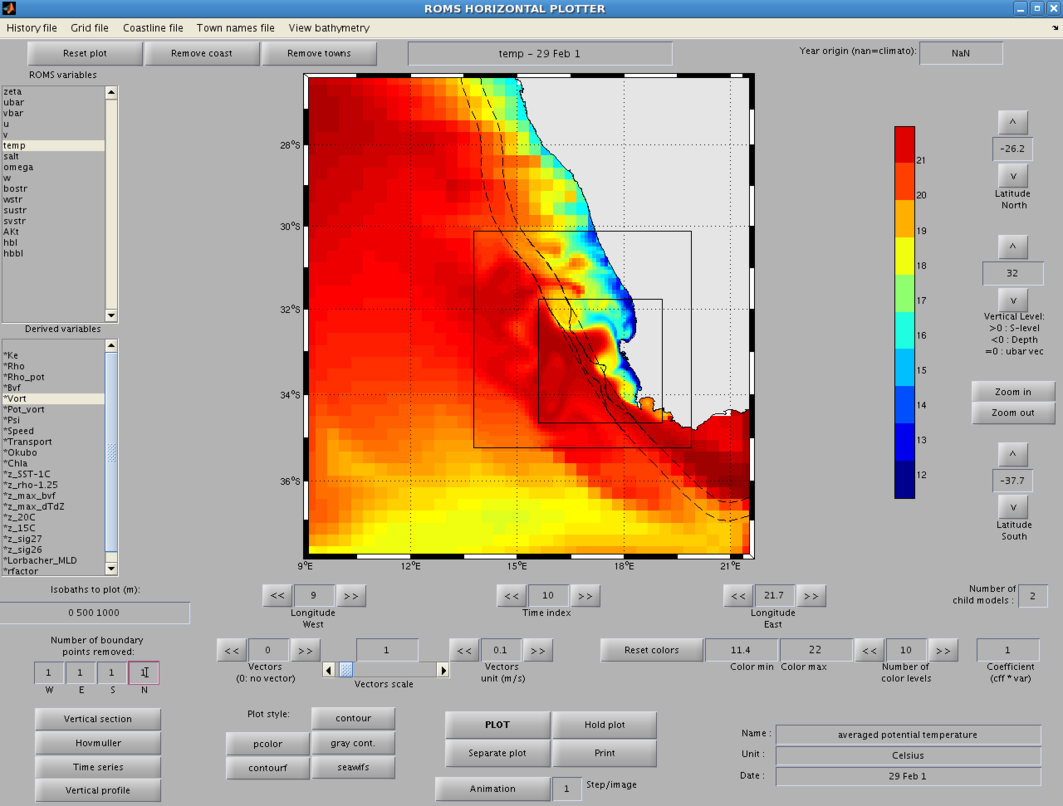
\includegraphics[width=0.9\textwidth]{Figures/romsgui_vizuM2.eps}
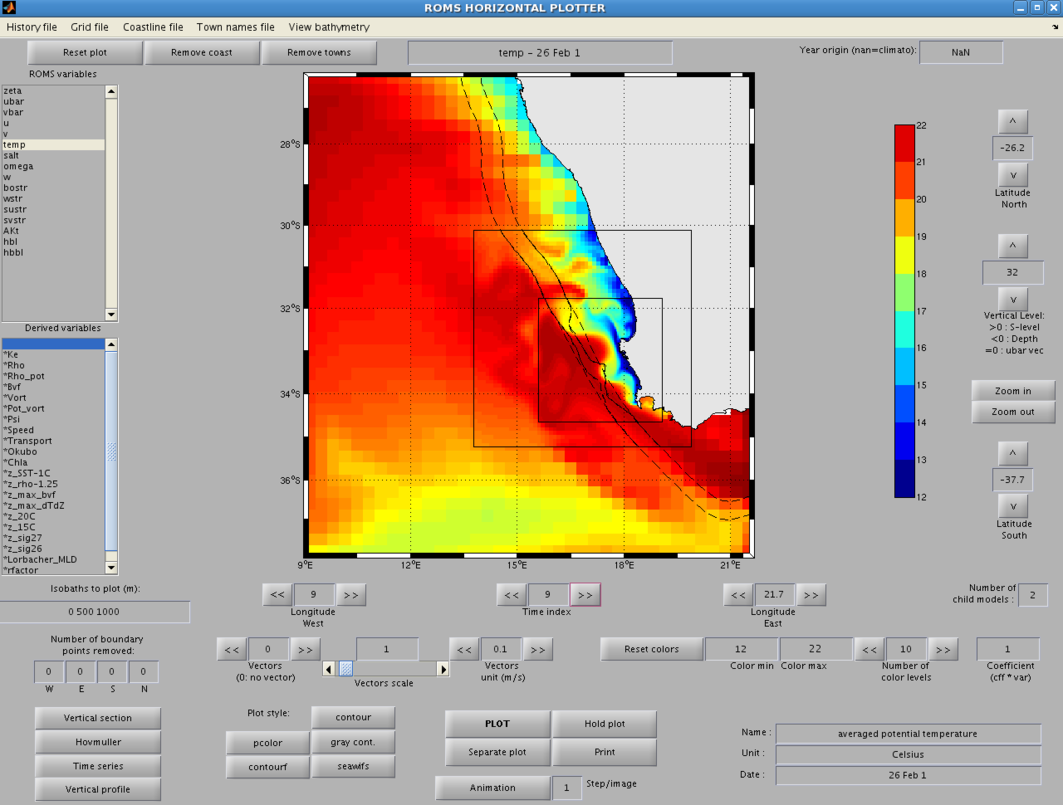
\includegraphics[width=0.9\textwidth]{Figures/romsgui_vizu_pagegarde.eps}
\vspace{1cm} \\
{July, 2010}
\end{center}
\chapter*{Introduction}
% This guide presents a series of Matlab routines which could be useful for the pre-
% and post-processing of oceanic regional ROMS simulations.

% This report is a basic users guide presenting the details of the methods and datasets
% are described in \citet{Pen07} and some

The Regional Ocean Modeling System (ROMS) is a new generation ocean circulation model
\citep{Shc03b} that has been specially designed for accurate simulations of regional
oceanic systems.  The reader is referred to \citet{Shc03a} and to \citet{Shc03b} for
a complete description of the model.  ROMS has been applied for the regional
simulation of a variety of different regions of the world oceans
\citep[e.g.][]{Bla02,Dil03,Hai00,Mac02,Mar03,Pen01}. \\

To perform a regional simulation using ROMS, the modeler needs to provide several
data files in a specific format: horizontal grid, bottom topography, surface forcing,
lateral boundary conditions... He also needs to analyze the model outputs. The tools
which are described here have been designed to perform these tasks.  The goal is to
be able to build a standard regional model configuration in a minimum time. \\

In the first chapter, the system requirements and the installation process are
exposed. A short note on ROMS model is presented in chapter 2. A tutorial on the use
of ROMSTOOLS is shown in the third section. Tidal simulations, inter-annual
simulations, nesting tools, biology and operational regional modeling are presented
in section 4,
5, 6, 7 and 8. \\

In the second chapter, some details of the IRD version of ROMS new release, named
roms\_agrif $2.0$, using the AGRIF nesting procedure are presented. \\
First, the new AGRIF 2-ways nesting procedure implemented in the code is described,
then new numerical and physical schemes and parametrization are exposed. Then a
changelog section since the last roms\_agrif $1.0$ offical version is presented.
Finally, the cpp-keys, parameters and input files are described in details to
correctly configure the model options.


\newpage
\tableofcontents
\newpage
\chapter{ROMSTOOLS matlab toolbox}
\section{Installation}
\subsection{System requirement}
This toolbox has been designed for Matlab. It needs at least 
2 Gbites of disk space. It has been tested on several 
Matlab versions ranging from Matlab6 to Matlab2006a. It has been 
mostly tested on Linux workstations, but it could be used 
on any platform if a NetCDF and a LoadDAP  Matlab Mex files  
are provided. The NetCDF Matlab Mex file is needed to read 
and write into NetCDF files and it can be found at the web 
location: http://mexcdf.sourceforge.net/. The LoadDAP Matlab Mex file
is used to download data from OpenDAP servers for inter-annual and forecast 
simulations. It can be found at the web location: 
http://www.opendap.org/download/ml-structs.html. The Matlab 
LoadDAP Mex file provides a way to read any OpenDAP-accessible 
data into Matlab. Note that the LibDAP library must be installed
on your system before installing LoadDAP. Details can be found 
at the web location: http://www.opendap.org. MexCDF and LoadDAP mex 
files are provided for Linux (system FEDORA 32bits: mexcdf and 
Opendap\_tools/FEDORA ; system CENTOS or FEDORA 64bits: 
mexnc and Opendap\_tools/FEDORA\_X64), but they are not working 
on all the plateforms.

All the other necessary Matlab toolboxes (i.e. air-sea, mask, 
netcdf or m\_map...) are included in the ROMSTOOLS package. 
Global datasets, such as topography \citep{Smi97}, 
hydrography \citep{Con02} or surface fluxes \citep{Das94}, are 
also included.

\subsection{Getting the files}

All the necessary compressed tar files (XXX.tar.gz) containing 
the Matlab programs, several datasets  and other toolboxes and 
softwares needed by ROMSTOOLS are located at:
\begin{center}
http://roms.mpl.ird.fr/Roms\_tools/index.html 
\end{center}
For the ROMS source code you should download ROMS\_AGRIF version
V2.0.\\\\\\\\\\\\


\subsection{Extracting the files}

Download all the compressed tar files. Uncompress and untar all 
the files (gunzip and tar -xvf). You should obtain the following 
directory tree : \\
\\
Roms\_tools

$|$-- Aforc\_NCEP

$|$-- Aforc\_QuikSCAT

$|$-- air\_sea 

$|$-- COADS05  

$|$-- Compile

$|$-- Diagnostic\_tools

$|$-- Documentation

$|$\hspace{0.5cm}$|$-- User\_guide

$|$-- Forecast\_tools

$|$-- mask

$|$-- mex60

$|$-- mexcdf

$|$\hspace{0.5cm}$|$-- mexnc

$|$\hspace{1.0cm}$|$-- private

$|$\hspace{1.0cm}$|$-- src

$|$\hspace{1.0cm}$|$-- tests

$|$\hspace{1.0cm}$|$-- win32

$|$\hspace{1.0cm}$|$-- win64

$|$\hspace{0.5cm}$|$-- netcdf\_toolbox

$|$\hspace{1.0cm}$|$-- README

$|$\hspace{1.0cm}$|$-- ChangeLog

$|$\hspace{1.0cm}$|$-- netcdf

$|$\hspace{2.0cm}$|$-- @listpick

$|$\hspace{2.0cm}$|$-- @ncatt

$|$\hspace{2.0cm}$|$-- @ncbrowser

$|$\hspace{2.0cm}$|$-- @ncdim

$|$\hspace{2.0cm}$|$-- @ncvar

$|$\hspace{2.0cm}$|$-- @netcdf

$|$\hspace{2.0cm}$|$-- @ncitem

$|$\hspace{2.0cm}$|$-- @ncrec

$|$\hspace{2.0cm}$|$-- nctype

$|$\hspace{2.0cm}$|$-- ncutility

$|$\hspace{2.0cm}$|$-- ncsources

$|$\hspace{0.5cm}$|$-- snctools (\textit{unused yet})

$|$-- m\_map

$|$\hspace{0.5cm}$|$-- private

$|$-- Nesting\_tools

$|$-- netcdf\_g77

$|$-- netcdf\_ifc

$|$-- netcdf\_x86\_64

$|$-- Oforc\_OGCM

$|$-- Opendap\_tools

$|$\hspace{0.5cm}$|$-- FEDORA

$|$\hspace{0.5cm}$|$-- FEDORA\_X64

$|$-- Preprocessing\_tools

$|$-- Roms\_Agrif

$|$\hspace{0.5cm}$|$-- AGRIFZOOM

$|$\hspace{0.5cm}$|$\hspace{0.5cm}$|$-- AGRIF\_FILES

$|$\hspace{0.5cm}$|$\hspace{0.5cm}$|$-- AGRIF\_INC

$|$\hspace{0.5cm}$|$\hspace{0.5cm}$|$-- AGRIF\_OBJS

$|$\hspace{0.5cm}$|$\hspace{0.5cm}$|$-- AGRIF\_YOURFILES

$|$\hspace{0.5cm}$|$\hspace{0.5cm}$|$-- LIB.clean

$|$-- Run

$|$\hspace{0.5cm}$|$-- DATA


$|$\hspace{0.5cm}$|$-- FORECAST

$|$\hspace{0.5cm}$|$-- ROMS\_FILES

$|$\hspace{0.5cm}$|$-- SCRATCH

$|$\hspace{0.5cm}$|$-- TEST\_CASES

$|$-- SeaWifs

$|$-- SST\_pathfinder

$|$-- Tides

$|$-- Topo

$|$\hspace{0.5cm}$|$-- Matlab

$|$-- TPX06

$|$-- TPX07

$|$-- Visualization\_tools

$|$-- WOA2001

$|$-- WOA2005
\\
\\
Definition of the different directories :
\begin{itemize}
\item Aforc\_NCEP : Scripts for the recovery of surface forcing data 
      (based on NCEP reanalysis) for inter-annual simulations.
\item Aforc\_QuikSCAT : Scripts for the recovery of wind stress from 
      satellite scatterometer data (QuickSCAT).
\item COADS05 : Directory of the surface fluxes global monthly 
      climatology at $0.5^\circ$ resolution \citep{Das94}.
\item Compile : Empty scratch directory for ROMS compilation.
\item Diagnostic\_tools : A few Matlab scripts for animations and
      basic statistical analysis.
\item Documentation : Location of the ROMSTOOLS user guide.
\item Forecast\_tools : Scripts for the generation of an operational
      modeling system 
\item mask : Land mask edition toolbox developed by A.Y. Shcherbina.
\item mex60 : Matlab NetCDF interface for 32 \& 64 bits Linux architectures and old
  matlab version : 6 and before.
\item mexcdf/mexnc : Matlab NetCDF interface for 32 \& 64 bits Linux architectures,
  MatlabR14sp1 until R2008a (http://mexcdf.sourceforge.net/downloads/mexcdf-R2008a.r2691.zip) \\
  For next releases of Matlab, R2008b, R2009a, it is more simpler, either use the native NetCDF
  toobox of matlab or use the last release of mexcf at the same url for version
  after R2008a.(http://mexcdf.sourceforge.net/downloads/mexcdf.r2802.zip)
\item mexcdf/netcdf\_toolbox : The Matlab NetCDF toolbox available in the same mexcdf
  package.
\item m\_map : The Matlab mapping toolbox 
      (http://www2.ocgy.ubc.ca/$\sim$rich/map.html).
\item Nesting\_tools : Preprocessing tools used to prepare nested
      models.
\item netcdf\_g77 : The NetCDF Fortran library for Linux, compiled using g77\\
      (http://www.unidata.ucar.edu/packages/netcdf/index.html).
\item netcdf\_ifc : The NetCDF Fortran library for Linux, compiled with ifort. 
      The Intel Fortran Compiler (ifort) is available at \\
      http://www.intel.com/software/products/compilers/flin/noncom.htm.
\item netcdf\_x86\_64 : The NetCDF Fortran library for Linux, compiled with ifort
      on a 64 bits architecture.
\item Oforc\_OGCM : Scripts for the recovery of initial and lateral boundary 
      conditions from global OGCMs (SODA \citep{Car05} or ECCO \citep{Sta99}) for 
      inter-annual simulations.
\item Opendap\_tools : LoadDAP mexcdf and several scripts to automatically
      download data over the Internet.
\item Preprocessing\_tools : Preprocessing Matlab scripts (make\_grid.m, 
      make\_forcing, etc...).
\item Roms\_Agrif : ROMS Fortran sources.
\item Run : Working directory. This is where the ROMS input files
      are generated and where the model is running.
\item SeaWifs : surface chlorophyll-a climatology based on SeaWifs observations.
\item SST\_pathfinder : Directory of a higher resolution SST climatology 
      \citep{Rey94} for the thermal correction term.
\item Tides : Matlab routines to prepare ROMS tidal simulations. Tidal data
      are derived from the Oregon State University global models of ocean tides 
      TPXO6 and TPXO7 \citep{Egb02}: 
      http://www.oce.orst.edu/research/po/research/tide/global.html.
\item Topo : Location of the global topography dataset at $2'$ resolution
      \citep{Smi97}. Original data can be found at:
      http://topex.ucsd.edu/cgi-bin/get\_data.cgi
\item TPX06 : Directory of the global model of ocean tides TPXO6 \citep{Egb02}.
\item TPX07 : Directory of the global model of ocean tides TPXO7 \citep{Egb02}.
\item Visualization\_tools : Matlab scripts for the ROMS visualization
      graphic user interface.
\item WOA2001 : World Ocean Atlas 2001 global dataset 
      (monthly climatology at $1^\circ$ resolution) \citep{Con02}.
\item WOA2005 : World Ocean Atlas 2005 global dataset 
\item WOAPISCES : World Ocean Atlas Global dataset for biogeochemical PISCES data

\end{itemize}



\section{LibDAP and  LoadDAP}\label{sec:libdap}
It is sometimes difficult to compile LoadDAP.  LibDAP must be installed before
installing LoadDAP. You have to declare the LibDAP binary and library in tour
~/.bashrc with th command PATH and LD\_LIBRARY\_PATH. Once, compile and install
LoadDAP.

Here are a few instructions for the installation of these libraries:\\
\begin{itemize}
\item Download libDAP and loadDAP tar.gz version at the web location
http://www.opendap.org
\item To build the libDAP library, follow these steps:\\
\item log you as a root
\item Uncompress and untar the file libdap.tar.gz (gunzip and tar -xvf)
\item $>$: cd libdap\_directory
\item Type './configure' at the prompt. Some libraries must be installed 
on your system to successfully run configure and build libDAP library : libcurl 
(http://curl.haxx.se/) and libxml2 (http://xmlsoft.org/).\\
Example:\\
------------------------------------------------------------------------------------------\\
checking for a BSD-compatible install... /usr/bin/install -c\\
checking whether build environment is sane... yes\\
checking whether make sets (MAKE)... yes\\
checking build system type... i686-pc-linux-gnu\\
checking host system type... i686-pc-linux-gnu\\
checking for gawk... (cached) mawk\\
checking for g++... g++\\
checking for C++ compiler default output file name... a.out\\
...\\
config.status: dods-datatypes.h is unchanged\\
config.status: executing depfiles commands\\
------------------------------------------------------------------------------------------\\
\item Type 'make' to build the library.\\
Example :\\
------------------------------------------------------------------------------------------\\
make[1]: Entering directory '/home/tropic/tan/soft/libdap-3.6.2'\\
Making all in gl\\
make[2]: Entering directory '/home/tropic/tan/soft/libdap-3.6.2/gl'\\
make  all-am\\
make[3]: Entering directory '/home/tropic/tan/soft/libdap-3.6.2/gl'\\
...\\
------------------------------------------------------------------------------------------\\
\item Type 'make check' to run the tests. To pass this step you 
must have DejaGNU framework (GNU FTP mirror list:
http://www.gnu.org/prep/ftp.html).\\
Example :\\
------------------------------------------------------------------------------------------\\
make[1]: Entering directory `/home/tropic/tan/soft/libdap-3.6.2/gl'\\
dejagnu\_driver.sh\\
...\\
Test Run By tan on Thu Jul 19 11:19:02 2007\\
Native configuration is i686-pc-linux-gnu\\
                ===== das-test tests =====\\
		Running ...\\
                ===== das-test Summary =====\\		
                ===== dds-test tests =====\\
		Running ...\\
		===== dds-test Summary =====\\
                ===== expr-test tests =====\\
		Running ...\\
                ===== expr-test Summary =====\\
PASS: dejagnu\_driver.sh\\
==================\\
All 1 tests passed\\
==================\\
make[2]: Leaving directory `/home/tropic/tan/soft/libdap-3.6.2/tests'\\
make[1]: Leaving directory `/home/tropic/tan/soft/libdap-3.6.2/tests'\\
------------------------------------------------------------------------------------------\\
\item Type 'make install' to install the library. By default the files are installed under
/usr/local/lib/. You can specify a different root directory using the following control :
'make install root\_directory'.\\
\item Go to the .bashrc and add \\EXPORT LD\_LIBRARY\_PATH=\$LD\_LIBRARY\_PATH
: root\_directory.'\\

\item The installation of the loadDAP library is done as for libDAP. 
By default the files are installed under
/usr/local/share/.

\item Go in the .dodsrc file, add the PROXY\_SERVER configuration, if needed,
    for example PROXY\_SERVER http,proxy.legos.obs-mip.fr:$3128$
\end{itemize}

\section{Future plans}
\begin{itemize}
\item A graphic user interface could be useful for the preprocessing tools.
\item There is need for an improvement of the extrapolation and interpolation
methods.
\end{itemize}

\section{Warnings}
\begin{itemize}
\item Since Geostrophy is used to obtain the horizontal currents for
the lateral boundary conditions, this method should be applied with 
care close to the Equator. An extrapolation of the currents outside 
an equatorial band (2$^\circ$S-2$^\circ$N) is performed to get an 
approximation of the equatorial currents.
\item On extended grids, the objective analysis used for data 
extrapolation can be relatively costly in memory and CPU time. 
The "nearest" Matlab function that is less costly can be used instead.
If the computer starts to swap, you should think of reducing the 
dimension of your model's domain.
\end{itemize}
\newpage


\section{Tutorial : the Southern Benguela example}
This section presents the essential steps for preparing and running a regional ROMS
simulation. This is done following the example of a model of the Southern Benguela at
low resolution and using climatological forcing at surface and boundaries.
 
\subsection{Getting started : Processing input files}

Once the installation has been successful, launch a Matlab session in
the directory: $\sim$/Roms\_tools/Run. Run the start.m script to set
the Matlab paths for this session.

% The start.m script also makes the difference between 32 bits and 64 bits Linux
% architectures
% and adjusts the paths in consequence: \\
% \\
% $>$ : cd Roms\_tools/Run \\
% $>$ : matlab \\
% $<$ M A T L A B $>$...\\
% $>>$ start \\
% Add the paths of the different toolboxes... \\
% Arch : x86\_64 - Matlab version : 12 \\
% Use of mex60 and loaddap in 32 bits. \\
% $>>$ \\
% \\

In this step of this installation, you have to know a few things concerning your
matlab setup and tour computer environnmemnt:
\begin{itemize}
\item What is the architecture of my machine 32 or 64 bits ? For that do uname -a.
\item What are the native matlab installation library that I have ?
\item Do I need to install manually the netcdf library ?
\item Do I need to add manually the m\_map library ? For these questions, edit your
  matlab path with the matlab command \textbf{path}. \\
\end{itemize}

In the Roms\_tools, some netcdf librarie for matlab are provided : 
\begin{itemize}
\item mex60 : matlab12 (old) and $32$ bits architecture
\item mexnc : matlab7 and $64$ bits architecture
%\item mexnc32 : matlab7 and $32$ bits architecture... to do
%\item mexnc64 : matlab7 and $64$ bits architecture... to do
\end{itemize}

In the Roms\_tools, some "opendap" bins and librarys are also provided :
\begin{itemize}
\item Opendap\_tools$/$FEDORA : LibDAP and LoadDAP bin and library for Fedora Linux
  distribution, $32$ bits architecture
\item Opendap\_tools$/$FEDORA\_X64 : Same for $64$ bits architecture.
\end{itemize}
However, if your Linux distribution differs from Fedora, the best is to compile and
install by your own the LibDAP and LoadDAP. \\


You are now ready to create a new configuration.  It is important to
respect the order of the following preprocessing steps: make\_grid,
make\_forcing, make\_clim.  For all the preprocessing steps, there is
only one file to edit : $\sim$/Roms\_tools/Run/romstools\_param.m .
This file contains the necessary parameters for the generation of the
ROMS input NetCDF files.  The first section in romstools\_param.m
defines the general parameters, such as title, working directories or
file names:
\\ \\
\%\%\%\%\%\%\%\%\%\%\%\%\%\%\%\%\%\%\%\%\%\%\\
\%\\
\% 1- General parameters\\
\%\\
\%\%\%\%\%\%\%\%\%\%\%\%\%\%\%\%\%\%\%\%\%\%\\
\%\\
\%  ROMS title names and directories\\
\%\\
ROMS\_title  = 'Benguela Test Model';\\
ROMS\_config = 'Benguela\_LR';\\
\%\\
ROMSTOOLS\_dir = '../';\\
\%\\
\%\\ Run directory
\%\\
RUN\_dir=[ROMSTOOLS\_dir,'Run/'];\\
\%\\
ROMS\_files\_dir=[RUN\_dir,'ROMS\_FILES/'];\\
\%\\
\%  Global data directory (etopo, coads, datasets download from ftp, etc..)\\
\%\\
DATADIR=ROMSTOOLS\_dir; 
\%\\
\%  Forcing data directory (ncep, quikscat, datasets download with opendap, etc..)\\
\%\\
FORC\_DATA\_DIR = [RUN\_dir,'DATA/'];\\
\%\\
\% ROMS file names (grid, forcing, bulk, climatology, initial)\\
\%\\
eval(['!mkdir ',ROMS\_files\_dir]) \\
\%\\
bioname=[ROMS\_files\_dir,'roms\_frcbio.nc'];  \%Iron Dust forcing file with PISCES \\
grdname=[ROMS\_files\_dir,'roms\_grd.nc'];\\
frcname=[ROMS\_files\_dir,'roms\_frc.nc'];\\
blkname=[ROMS\_files\_dir,'roms\_blk.nc'];\\
clmname=[ROMS\_files\_dir,'roms\_clm.nc'];\\
ininame=[ROMS\_files\_dir,'roms\_ini.nc'];\\
oaname =[ROMS\_files\_dir,'roms\_oa.nc'];    \% oa file  : intermediate file not used\\
\%            in roms simulations\\
bryname=[ROMS\_files\_dir,'roms\_bry.nc'];\\
Zbryname=[ROMS\_files\_dir,'roms\_bry\_Z.nc'];\% Zbry file: intermediate file not used\\
\%            in roms simulations\\
\%\\
frc\_prefix=[ROMS\_files\_dir,'roms\_frc'];   \% generic bulk forcing file name \\
\% for inter-annual roms simulations (NCEP or GFS)\\
blk\_prefix=[ROMS\_files\_dir,'roms\_blk'];   \% generic forcing file name\\
\% for inter-annual roms simulations (NCEP or GFS)\\
\%\\
\% Objective analysis decorrelation scale [m]\\
\% (if Roa=0: simple extrapolation method; crude but much less costly)\\
\%\\
\%Roa=300e3;\\
Roa=0;\\
\%\\
interp\_method = 'linear';           \% Interpolation method: 'linear' or 'cubic'\\
\%\\
makeplot     = 1;                 \% 1: create a few graphics after each preprocessing step\\
\%\\
\%\%\%\%\%\%\%\%\%\%\%\%\%\%\%\%\%\%\%\%\%\%\%\%\%\%\%\%\%\%\%\%\%\%\%\%\%\%\\
\\
Variables description:
\begin{itemize}
\item title='Benguela Test Model' : General title. You can give any name 
you want for your configuration.
\item ROMS\_config = 'Benguela\_LR' : Name of the configuration. This is used for the storage of
NCEP or OGCM data for a specific configuration.
\item ROMSTOOLS\_dir = '../' : "Roms\_tools" directory.
\item RUN\_dir=[ROMSTOOLS\_dir,'Run/'] : Roms\_tools/Run directory. This is where all 
the work is done.
\item ROMS\_files\_dir=[RUN\_dir,'ROMS\_FILES/'] : Roms\_tools/Run/ROMS\_FILES/ directory.
This is where ROMS input NetCDF files are stored.
\item ROMS\_files\_dir=[RUN\_dir,'ROMS\_FILES/'] : 
\item DATADIR=ROMSTOOLS\_dir;  : Global data directory (ETOPO, COADS, datasets download from ftp, etc..)
\item FORC\_DATA\_DIR = [RUN\_dir,'DATA/'] :  Forcing data directory (NCEP, QUIKSCAT, datasets downloaded with opendap, etc..)

\item bioname=[ROMS\_files\_dir,'roms\_frcbio.nc'] :  Name of the ROMS input NetCDF Iron dust forcing file for  PISCES biogeochemical model.
\item grdname=[ROMS\_files\_dir,'roms\_grd.nc'] : Name of the ROMS input NetCDF grid file.
This is where the horizontal grid parameters are stored. In general, we follow 
the style : XXX\_grd.nc.
\item frcname=[ROMS\_files\_dir,'roms\_frc.nc'] : : Name of the ROMS input NetCDF forcing file.
This is where the surface forcing variables (such as wind stress) are stored. In general, we 
follow  the style : XXX\_frc.nc.
\item blkname=[ROMS\_files\_dir,'roms\_blk.nc'] : Name of the ROMS input NetCDF bulk file.
This is where the atmospheric variables used for the bulk parametrization (such as air temperature) 
are stored. In general, we follow  the style : XXX\_blk.nc.
\item clmname=[ROMS\_files\_dir,'roms\_clm.nc'] : Name of the ROMS input NetCDF climatology file.
This is where ROMS prognostic variables (u,v, temp, salt, ubar, vbar, zeta) for lateral boundary 
and interior nudging are stored. This file can be large because variables are stored for all the 
ROMS grid interior points. It is called "a climatology file" because this was the file used in 
the past for the restoring of the ROMS solution towards an in-situ climatology (such as Levitus 
for example). In general, we follow the style : XXX\_clm.nc.
\item ininame=[ROMS\_files\_dir,'roms\_ini.nc'] : Name of the ROMS input NetCDF initial file.
This is where ROMS prognostic variables (u,v, temp, salt, ubar, vbar, zeta) are stored 
for the initial conditions. In general, we follow the style : XXX\_ini.nc.
\item oaname =[ROMS\_files\_dir,'roms\_oa.nc'] : Name of an intermediate file which is not
used by ROMS. This is equivalent to the climatology file, but on a z vertical coordinate.
Firstly, the variables are horizontally interpolated to create a roms\_oa.nc file (a OA file). 
Then, they are vertically interpolated on the ROMS s-coordinate for the climatology
file. In general, we follow the style : XXX\_oa.nc.
\item bryname=[ROMS\_files\_dir,'roms\_bry.nc'] : Name of the ROMS input NetCDF boundary file.
This is an alternative of the climatology file. In this case, variables are only stored for 
the lateral boundaries. In general, we follow the style : XXX\_bry.nc.
\item Zbryname=[ROMS\_files\_dir,'roms\_bry\_Z.nc'] : Intermediate file on a z coordinate
for the boundary file. In general, we follow the style : XXX\_bry\_Z.nc.
\item frc\_prefix=[ROMS\_files\_dir,'roms\_frc'] : First part of the forcing file names in
the case of inter\_annual simulations. In this case, a separate file is created for each month.
For example, a forcing file based on NCEP for January 2000 is : roms\_frc\_NCEP\_Y2000M1.nc
\item blk\_prefix=[ROMS\_files\_dir,'roms\_blk'] : First part of the bulk file names in
the case of inter\_annual simulations. In this case, a separate file is created for each month.
For example, a bulk file based on NCEP for January 2000 is : roms\_blk\_NCEP\_Y2000M1.nc
%
\item Roa=0 : Decorrelation length scale in meters for the objective analysis (300 km
is a reasonable value for the employed datasets). If Roa=0, the "nearest" Matlab extrapolation
method is used instead of an objective analysis. This is much less costly, but the 
results might be at a lower quality.
\item interp\_method = 'cubic' : Horizontal interpolation method used after the objective 
analysis. It can be linear or cubic.
\item makeplot     = 1 : Select to generate images after each step of the preprocessing.
\end{itemize}


\subsection{Building the grid}

The part of the file romstools\_param.m that you should be edit is :
\\ \\
\%\%\%\%\%\%\%\%\%\%\%\%\%\%\%\%\%\%\%\%\%\%\\
\%\\
\% 2-Grid parameters\\
\%   used by make\_grid.m (and others..)\\
\%\\
\%\%\%\%\%\%\%\%\%\%\%\%\%\%\%\%\%\%\%\%\%\%\\
\%\\
\% Grid dimensions:\\
\%\\
lonmin =  8;   \% Minimum longitude [degree east]\\
lonmax = 22;   \% Maximum longitude [degree east]\\
latmin = -38;   \% Minimum latitude  [degree north]\\
latmax = -26;   \% Maximum latitude  [degree north]\\
\%\\
\% Grid resolution [degree]\\
\%\\
dl = 1/3;\\
\%\\
\% Number of vertical Levels (! should be the same in param.h !)\\
\%\\
N = 32;\\
\%\\
\%  Vertical grid parameters (! should be the same in roms.in !)\\
\%\\
theta\_s = 8.;\\
theta\_b = 0.;\\
hc      =10.;\\
\%\\
\% Minimum depth at the shore [m] (depends on the resolution,\\
\% rule of thumb: dl=1, hmin=300, dl=1/4, hmin=150, ...)\\
\% This affect the filtering since it works on grad(h)/h.\\
\%\\
hmin = 75;\\
\%\\
\% Maximum depth at the shore [m] (to prevent the generation\\
\% of too big walls along the coast)\\
\%\\
hmax\_coast = 500;\\
\%\\
\%  Topography netcdf file name (ETOPO 2 or any other netcdf file\\
\%  in the same format)\\
\%\\
topofile = [DATADIR,'Topo/etopo2.nc'];\\
\%\\
\% Slope parameter (r=grad(h)/h) maximum value for topography smoothing\\
\%\\
rtarget = 0.25;\\
\%\\
\% Number of pass of a selective filter to reduce the isolated\\
\% seamounts on the deep ocean.\\
\%\\
n\_filter\_deep\_topo=4;\\
\%\\
\% Number of pass of a single hanning filter at the end of the\\
\% smoothing procedure to ensure that there is no 2DX noise in the \\
\% topography.\\
\%\\
n\_filter\_final=2;\\
\%\\
\%  GSHSS user defined coastline (see m\_map) \\
\%  XXX\_f.mat    Full resolution data\\
\%  XXX\_h.mat    High resolution data\\
\%  XXX\_i.mat    Intermediate resolution data\\
\%  XXX\_l.mat    Low resolution data\\
\%  XXX\_c.mat    Crude resolution data\\
\%\\
coastfileplot = 'coastline\_l.mat';\\
coastfilemask = 'coastline\_l\_mask.mat';\\
\\
Variables description:
\begin{itemize}
\item lonmin =  8 : Western limit of the grid in longitude [-360$^\circ$, 360$^\circ$]. 
The grid is rectangular in latitude/longitude.
\item lonmax = 22 : Eastern limit [-360$^\circ$, 360$^\circ$]. 
Should be superior to lonmin.
\item latmin = -38 : Southern limit of the grid in latitude [-90$^\circ$, 90$^\circ$].
\item latmax = -26 : Northern limit [-90$^\circ$, 90$^\circ$].
Should be superior to latmin.
\item l = 1/3 : Grid longitude resolution in degrees. The latitude spacing is deduced to
obtain an isotropic grid using the relation: $d\phi=dl\cos(\phi)$.
\item N = 32 : Number of vertical levels. Warning! N has to be also 
defined in the file : $\sim$/Roms\_tools/Run/param.h before compiling
the model.
\item theta\_s = 6. : Vertical S-coordinate surface stretching parameter. 
When building the climatology and initial ROMS files, we have to define
the vertical grid. Warning! The different vertical grid parameters should 
be identical in this file and in the ROMS input file (i.e. 
$\sim$/Roms\_tools/Run/roms.in).
This is a serious cause of bug.
The effects of theta\_s, theta\_b, hc, and N can be tested 
using the Matlab script : \\
$\sim$/Roms\_tools/Preprocessing\_tools/test\_vgrid.m.
\item theta\_b = 0. : Vertical S-coordinate bottom stretching parameter.
\item hc      = 10. : Vertical S-coordinate $H_c$ parameter. It gives approximately the
transition depth between the horizontal surface levels and the bottom terrain following
levels. It should be inferior to hmin.
\item hmin = 75 : Minimum depth in meters. The model depth is cut a this level 
to prevent, for example, the occurrence of model grid cells without water.
This does not influence the masking routines. At lower resolution, hmin should be 
quite large (for example 150m for dl=1/2). Otherwise, since topography smoothing 
is based on $\frac{\nabla h}{2h}$, the bottom slopes can be totally eroded.
\item hmax\_coast = 500 : Maximum depth under the mask. It prevents selected
isobaths (here 500 m) to go under the mask. If this is the case, 
this could be a source of problems
for western boundary currents (for example).
\item topofile = [ROMSTOOLS\_dir,'Topo/etopo2.nc'] : Default topography file. 
We are using here etopo2 \citep{Smi97}. 
\item rtarget = 0.25 : This variable control the maximum value of the $r$-parameter
that measures the slope of the sigma layers \citep{Bec93}:
$$
r=\frac{\nabla h}{2h}=\frac{h_{+1/2}-h_{-1/2}}{h_{+1/2}+h_{-1/2}}  
$$
To prevent horizontal pressure gradients errors, well known in
terrain-following coordinate models \citep{Han91}, realistic topography
requires some smoothing. Empirical results have shown that reliable
model results are obtained if $r$ does not exceed 0.2.
\item n\_filter\_deep\_topo=4 : Number of pass of a Hanning filter to prevent 
the occurrence of noise and isolated seamounts on deep regions.
\item n\_filter\_final=2 : Number of pass of a Hanning filter at the end of the
smoothing process to be sure that no noise is present in the topography.
\item coastfileplot = 'coastline\_l.mat' : Binary GSHSS coastal file used by m\_map
for graphical pruposes. The letter before ".mat" selects the coastline resolution.
f: Full resolution, h: High resolution, i: Intermediate resolution, l: Low resolution
c: Crude resolution.
\item coastfilemask = 'coastline\_l\_mask.mat' :  Binary file used
for the coastline in the masking toolbox.
\end{itemize}

Save romstools\_param.m and run make\_grid in the Matlab session :
\\ \\ 
$>>$\\
$>>$ make\_grid \\
 \\
You should obtain in the Matlab session:\\
------------------------------------------------------------------------------------------\\
Making the grid: ../Run/ROMS\_FILES/roms\_grd.nc \\
\\
Title: Benguela Test Model \\
\\
Resolution: 1/3 deg \\
\\
Create the grid file... \\
LLm = 41 \\
MMm = 42 \\
\\
Fill the grid file... \\
\\
Compute the metrics... \\
\\
Min dx=29.1913 km - Max dx=33.3244 km \\
Min dy=29.2434 km - Max dy=33.1967 km \\
\\
Fill the grid file... \\
\\
Add topography... \\
  ROMS resolution : 31.3 km \\
  Topography data resolution :  3.42 km \\
  Topography resolution halved 4 times \\
   New topography resolution :  54.6 km \\
Processing coastline\_l.mat ... \\
Do you want to use editmask ? y,[n]\\
 Apply a filter on the Deep Ocean to remove the isolated seamounts :\\
   4 pass of a selective filter.\\
 Apply a selective filter on log(h) to reduce grad(h)/h :\\
   13 iterations - rmax = 0.24381\\
 Smooth the topography a last time to prevent 2DX noise:\\
   2 pass of a hanning smoother.\\
 Write it down...\\
 Do a plot...\\
 $>>$\\
 ------------------------------------------------------------------------------------------\\
\\
You should keep the values of LLm and MMm during the process.
They will be necessary for the ROMS parameter file  
$\sim$/Roms\_tools/Run/param.h. In this test case,
LLm0 = 23 and MMm0 = 31. 

During the grid generation process, the question 
"Do you want to use editmask ? y,[n]" is asked. The default answer is n (for no).
If the answer is y (for yes), editmask, the  graphic interface developed 
by A.Y.Shcherbina, will be launched to manually edit the mask 
(Note that, for the moment, editmask is not working with matlab7 and mexnc).
Otherwise the
mask is generated from the unfiltered topography data. A procedure prevents 
the existence of isolated land (or sea) points.

Figure (\ref{fig:grid}) presents the
bottom topography obtained with make\_grid.m for the
Southern Benguela example. Note that at this low
resolution (1/3$^\circ$), the topography has been strongly
smoothed.

\begin{figure}[h!]
\centerline{\psfig{figure=make_grid_benguela.eps,width=12cm}}
\caption{Result of make\_grid.m for the Benguela example}
\label{fig:grid}
\end{figure}


\subsection{Getting the wind and other surface fluxes}

The next step is to create the file containing the different surface
fluxes. The part of the file romstools\_param.m that you should edit is :
\\
\\
\%\\
\%\%\%\%\%\%\%\%\%\%\%\%\%\%\%\%\%\%\%\%\%\%\%\%\%\%\%\\
\% 3-Surface forcing parameters\\
\%   used by make\_forcing.m and by make\_bulk.m\\
\%\\
\%\%\%\%\%\%\%\%\%\%\%\%\%\%\%\%\%\%\%\%\%\%\%\%\%\%\%\\
\% COADS directory (for climatology runs)\\
\%\\
coads\_dir=[ROMSTOOLS\_dir,'COADS05/'];\\
\%\\
\% COADS time (for climatology runs)\\
\%\\
coads\_time=(15:30:345); \% days: middle of each month\\
coads\_cycle=360;        \% repetition of a typical year of 360 days \\ 
\%\\
\%\%\%\%\%\%\%\%\%\%\%\%\%\%\%\%\%\%\%\%\%\%\%\%\%\%\%\\
\%\\
\% 3.1 Surface forcing parameters\\
\%   used by pathfinder\_sst.m\\
\%\\
\%\%\%\%\%\%\%\%\%\%\%\%\%\%\%\%\%\%\%\%\%\%\%\%\%\%\%\\
\%\\
pathfinder\_sst\_name=[ROMSTOOLS\_dir,...\\
                    'SST\_pathfinder/climato\_pathfinder.nc'];\\
\\
Variables description:
\begin{itemize}
\item coads\_dir=[ROMSTOOLS\_dir,'COADS05/'] : Directory where the global atlas of surface marine 
data at 1/2$^\circ$ resolution \citep{Das94} is located.
\item coads\_time=(15:30:345) : Time in days for the monthly climatology. It corresponds to the
middle of each month. ROMS uses this time to interpolate linearly the forcing variables in time.
\item coads\_cycle=360 : Duration on which the forcing variables are cycled. Here, for the sake
of simplicity, we are running the model on a repeating climatological year of 360 days.
\item pathfinder\_sst\_name=[ROMSTOOLS\_dir,SST\_pathfinder/climato\_pathfinder.nc'] : 
Directory of the  monthly climatology of sea surface temperature from Pathfinder satellite 
observations \citep{Cas99}. This can be used has an alternative of \citet{Das94} SST.
\end{itemize}


Save romstools\_param.m and run make\_forcing in the Matlab session :
\\  \\
$>>$\\
$>>$ make\_forcing\\\\
You should obtain :\\
------------------------------------------------------------------------------------------\\
Benguela Test Model\\
\\
 Read in the grid...\\
\\
 Create the forcing file...\\
Getting taux for time index 1\\
Getting tauy for time index 1\\
...\\
Make a few plots...\\
$>>$\\
------------------------------------------------------------------------------------------\\\\
This program can take a relatively long time to process all the forcing variables.
Figure (\ref{fig:forcing}) presents the wind stress vectors and wind stress norm 
obtained from the global atlas of surface marine 
data at 1/2$^\circ$ resolution \citep{Das94} at 4 different periods of the year.
\citet {Das94} sea surface temperature (SST) is used for the restoring term (dQdSST)
in the heat flux calculation. To improve the model solution it is possible to 
use a SST climatology at a finer resolution (9.28 km) \citep{Cas99}. To do 
so, you can run pathfinder\_sst.m in the Matlab session :
\\  \\
$>>$\\
$>>$ pathfinder\_sst\\\\\\\\
You should obtain :\\
------------------------------------------------------------------------------------------\\
 ... Month index: 1 \\
 ... Month index: 2 \\
...\\
$>>$\\
------------------------------------------------------------------------------------------\\\\
For the surface forcing, instead of directly prescribing the fluxes, it is possible 
to use a bulk formula to generate the surface fluxes from atmospheric variables 
during the model run. In this case, ROMS needs to be recompiled with the BULK\_FLUX
cpp key defined. To generate the bulk forcing file, you need to run make\_bulk
in the Matlab session :
\\ \\
$>>$\\
$>>$ make\_bulk\\\\
You should obtain :\\
------------------------------------------------------------------------------------------\\
Benguela Test Model\\
\\
 Read in the grid...\\
\\
 Create the bulk forcing file...\\
Getting sat for time index 1\\
Getting sat for time index 2\\
...\\
Make a few plots...\\
$>>$\\
------------------------------------------------------------------------------------------\\

\begin{figure}[h!]
\centerline{\psfig{figure=make_frcwind_benguela.eps,width=15cm}}
\caption{Wind stress[N.m$^{-2}$] obtained using make\_forcing.m for the Benguela example.}
\label{fig:forcing}
\end{figure}

\subsection{Getting the initial and the lateral boundary conditions}

The last preprocessing step consists in generating the files containing 
the necessary informations for the ROMS initial and lateral open boundaries 
conditions.
This script generates two files : the climatology file (XXX\_clm.nc) which gives 
the lateral boundary conditions, and the initial conditions file (XXX\_ini.nc). \\
The part which should be edited by the user in the file romstools\_param.m is. Note that you can 
you can add the variables for the NPZD or PISCES biogeochemical models. For that, 
define makebio or makepisces flags in the romstools\_param.m. \\
\\ \\
The part which should be edited by the user in the file romstools\_param.m is:
\\ \\
\%\%\%\%\%\%\%\%\%\%\%\%\%\%\%\%\%\%\%\%\%\%\%\%\%\%\%\%\%\%\%\\
\%\\
\% 4-Open boundaries and initial conditions parameters\\
\%   used by make\_clim.m, make\_biol.m, make\_bry.m\\
\%\\
\%\%\%\%\%\%\%\%\%\%\%\%\%\%\%\%\%\%\%\%\%\%\%\%\%\%\%\%\%\%\%\\
\%  Open boundaries switches (! should be consistent with cppdefs.h !)\\
\%\\
obc = [1 1 1 1]; \% open boundaries (1=open , [S E N W])\\
\%\\
\%  Level of reference for geostrophy calculation\\
\%\\
zref = -1000;\\
\%\\
\%  Switches for selecting what to process in make\_clim (1=ON)\\
\%  (and also in make\_OGCM.m and make\_OGCM\_frcst.m)\\
makeini=1;      \%1: process initial data\\
makeclim=1;     \%1: process lateral boundary data\\
makebry=0;      \%1: process boundary data\\
makebio=0;      \%1: process initial and boundary data for idealized NPZD type bio model
makepisces=0;  \%1: process initial and boundary data for PISCES biogeochemical model
\%\\
makeoa=1;       \%1: process oa data (intermediate file)\\
makeZbry=0;     \%1: process data in Z coordinate\\
\%\\
insitu2pot=1;   \%1: convert in-situ temperature into potential temperature\\
\%\\
\%  Day of initialization for climatology experiments (=0 : 1st January 0h)\\
\%\\
tini=0;\\  
\%\\
\% World Ocean Atlas directory (WOA2001 or WOA2005) \\
\%\\
woa\_dir=[ROMSTOOLS\_dir,'WOA2005/'];\\
\%\\
\% Surface chlorophyll seasonal climatology (WOA2001 or SeaWifs)\\
\%\\
chla\_dir=[ROMSTOOLS\_dir,'SeaWifs/'];\\
\%\\
\%  Set times and cycles for the boundary conditions:\\ 
\%   monthly climatology \\
\%\\
woa\_time=(15:30:345); \% days: middle of each month\\
woa\_cycle=360;        \% repetition of a typical year of 360 days\\  
\%\\

Variables description:
\begin{itemize}
\item obc=[1 1 1 1] : Switches to open (1=open) or close (0=wall) the lateral
boundaries [South East North West]. This is used for the application of mass
enforcement. Be aware, this should be compatible with the open boundary
CPP-switches in the file $\sim$/Roms\_tools/Run/cppdefs.h.
\item zref=-1000 : Depth [meters] of the level of no motion for the geostrophic 
velocities calculation.
\item makeini=1 : Switch to define if the initial file (roms\_ini.nc) is generated. 
Should be 1.
\item makeclim=1 : Switch to define if the climatology
 (lateral boundary conditions) file (roms\_clm.nc) is generated. Should be 1.
\item makeoa=1 : Switch to define if the OA (objective analysis; roms\_oa.nc)
 file is generated. This should be 1. The OA files are intermediate files
 where hydrographic data are stored on a ROMS horizontal grid but on
 a z vertical grid. The transformation into S-coordinate is done later.
 This file is not used by ROMS.
\item makebry=1 : Switch to define if the boundary file (roms\_bry.nc) is generated.
Used only with make\_bry.
\item makeZbry=1  : Switch to define if the boundary intermediate file on a z coordinate 
 (roms\_bry\_Z.nc) is generated. Used only with make\_bry.
\item makebio=1;      Switch to process initial and boundary data for idealized NPZD type bio model
\item makepisces=1 : Switch to process initial and boundary data for PISCES biogeochemical model
\item insitu2pot=1 : Switch defined if it is in-situ temperature that is provided.
In this case, in-situ temperature is converted into potential temperature.
\item tini=0 : Day of initialization in climatology experiments (15 = January 15).
\item woa\_dir=[ROMSTOOLS\_dir,'WOA2005/'] : Directory where the World Ocean
Atlas 2005 climatology \citep{Con02} is located. The World Ocean
Atlas 2001 climatology can also be used.
\item chla\_dir=[ROMSTOOLS\_dir,'SeaWifs/'] : Directory of the surface 
chlorophyll seasonal climatology.
\item woa\_time=(15:30:345) : Time in days for the WOA monthly climatology. 
It corresponds to the middle of each month. ROMS uses this variable to 
interpolate linearly the climatology variables in time.
\item woa\_cycle=360 : Duration on which the climatology variables are cycled. 
Here, for the sake of simplicity, we are running the model on a repeating climatological 
year of 360 days.
\end{itemize}
Save romstools\_param.m and run make\_clim in the Matlab session :
\\ \\
$>>$\\
$>>$ make\_clim \\\\
You should obtain :\\
------------------------------------------------------------------------------------------\\
 Making the clim: ../Run/ROMS\_FILES/roms\_clm.nc \\
 \\
 Title: Benguela Test Model \\
 \\
 Read in the grid...
 \\
 Create the climatology file... \\
 Creating the file : ../Run/ROMS\_FILES/roms\_clm.nc\\
 ...\\ 
 Make a few plots...\\ 
 $>>$\\
------------------------------------------------------------------------------------------\\
This program can also take quite a long time to run.
Figure (\ref{fig:clim}) presents 4 different sections
of temperature for the initial condition file for the 
Benguela example. The sections are in the X-direction (East-West), 
the first section is for the Southern part of the domain and the last one 
is for the Northern part of the domain.
\begin{figure}[h!]
\centerline{\psfig{figure=make_clim_benguela.eps,width=12cm}}
\caption{Result of make\_clim.m for the Benguela example}
\label{fig:clim}
\end{figure}

An alternative of using a climatology file is to create a boundary 
file. In this case, only boundary values are stored. The cpp key
FRC\_BRY should be defined and ROMS recompiled. Run make\_bry in 
the Matlab session :
\\ \\
$>>$\\
$>>$ make\_bry \\\\
You should obtain :\\
------------------------------------------------------------------------------------------\\
 Making the file: ../Run/ROMS\_FILES/roms\_bry.nc \\
 \\
 Title: Benguela Test Model \\
 \\
 Read in the grid... \\
... \\
------------------------------------------------------------------------------------------\\

\subsection{Compiling the model}

Once all the netcdf data files are ready (i.e. XXX\_grd.nc,
XXX\_frc.nc, XXX\_ini.nc, and XXX\_clm.nc), we can prepare ROMS for
compilation. All is done in the $\sim$/Roms\_tools/Run/ directory.

\subsubsection{Parameters of the configuration : param.h}
Edit the file $\sim$/Roms\_tools/Run/param.h.
The line which needs to be changed is:\\\\
\# elif defined BENGUELA\_LR

parameter (LLm0=41, MMm0=42, N=32)  ! $<--$ Southern Benguela Test Case\\
\#  else\\
\\
These are the values of the model grid size: LLm0 points in the X direction, MMm0
points in the Y direction and N vertical levels.  LLm0 and MMm0 are given by running
make\_grid.m, and N is defined in romstools\_param.m. The param.h parameters are
described in detail in section \ref{paramdesc}

\subsubsection{Numerical and physical options : cppdefs.h}
The second file to edit is $\sim$/Roms\_tools/Run/cppdefs.h.  This file defines the
CPP keys that are used by the the C-preprocessor when compiling ROMS. The
C-preprocessor selects the different parts of the Fortran code which needs to be
compiled depending on the defined CPP options. These options are separated in two
parts (the basic option keys and the advanced options keys) in cppdefs.h. All the
keys and their organization are described in section \ref{cppkeydesc}. \\

\subsubsection{Compilation script :  jobcomp}
ROMS can be compiled by running the UNIX tcsh script $\sim$/Roms\_tools/Run/jobcomp.
Jobcomp should be able to recognize your system. It has been tested on Linux, IBM,
Sun and Compaq systems. On Linux PCs, the default compiler is the GNU g77, but it is
possible to uncomment specific lines in jobcomp to use g95 or ifort.  The latter is
mandatory when using AGRIF and/or OPEN\_MP.  When changing the compiler you should
provide a corresponding NetCDF library.  Once the compilation is done, you should
obtain a new executable (roms) in the $\sim$/Roms\_tools/Run directory.  ROMS should
be recompiled each time param.h or cppdefs.h are changed.

\subsection{Running the model}
Edit the input parameter file: $\sim$/Roms\_tools/Run/roms.in.  The vertical grid
parameters (THETA\_S, THETA\_B, HC) should be identical to the ones in
romstools\_param.m.  Otherwise, the other default values should not be changed.  The
definition of all the input variables is given at the start of each ROMS simulation.
To run the model, type in directory $\sim$/Roms\_tools/Run/ : ./roms roms.in.  The
description of the namelist roms.in is descibed in details in section \ref{namelistdesc}

On the screen, you should check the Cu\_max parameter: if it is greater than 1 you
are violating the CFL criterion. In this case, you should reduce the time step.
\\
Example of model run:\\
\\
$>$ : ./roms roms.in
\\\\
You should obtain :\\
------------------------------------------------------------------------------------------\\
Southern Benguela\\
480  ntimes   Total number of timesteps for 3D equations.\\
5400.00  dt       Timestep [sec] for 3D equations\\
60  ndtfast  Number of 2D timesteps within each 3D step.\\
1  ninfo    Number of timesteps between runtime diagnostics.\\
\\
6.000E+00  theta\_s  S-coordinate surface control parameter.\\
0.000E+00  theta\_b  S-coordinate bottom control parameter.\\
1.000E+01  Tcline   S-coordinate surface/bottom layer width used in\\
vertical coordinate stretching, meters.\\
Grid File:  ROMS\_FILES/roms\_grd.nc\\
Forcing Data File:  ROMS\_FILES/roms\_frc.nc\\
Bulk Data File:  ROMS\_FILES/roms\_blk.nc\\
Climatology File:  ROMS\_FILES/roms\_clm.nc\\
Initial State File:  ROMS\_FILES/roms\_ini.nc    Record:  1\\
Restart File:  ROMS\_FILES/roms\_rst.nc    nrst =   480    rec/file:   -1\\
History File:  ROMS\_FILES/roms\_his.nc  Create new: T  nwrt = 480  rec/file =  0\\
1  ntsavg      Starting timestep for the accumulation of output\\
time-averaged data.\\
48  navg        Number of timesteps between writing of time-averaged\\
data into averages file.\\
Averages File:  ROMS\_FILES/roms\_avg.nc rec/file =  0\\
\\
Fields to be saved in history file: (T/F)\\
T  write zeta  free-surface.\\
F  write UBAR  2D U-momentum component.\\
F  write VBAR  2D V-momentum component.\\
F  write U     3D U-momentum component.\\
F  write V     3D V-momentum component.\\
F  write T(1)  Tracer of index 1.\\
F  write T(2)  Tracer of index 2.\\
\\
F  write RHO   Density anomaly.\\
F  write Omega Omega vertical velocity.\\
F  write W     True vertical velocity.\\
F  write Akv   Vertical viscosity.\\
F  write Akt   Vertical diffusivity for temperature.\\
F  write Aks   Vertical diffusivity for salinity.\\
F  write Hbl   Depth of KPP-model boundary layer.\\
F  write Bostr Bottom Stress.\\
\\
Fields to be saved in averages file: (T/F)\\
T  write zeta  free-surface.\\
T  write UBAR  2D U-momentum component.\\
T  write VBAR  2D V-momentum component.\\
T  write U     3D U-momentum component.\\
T  write V     3D V-momentum component.\\
T  write T(1)  Tracer of index 1.\\
T  write T(2)  Tracer of index 2.\\
\\
F  write RHO   Density anomaly\\
T  write Omega Omega vertical velocity.\\
T  write W     True vertical velocity.\\
F  write Akv   Vertical viscosity\\
T  write Akt   Vertical diffusivity for temperature.\\
F  write Aks   Vertical diffusivity for salinity.\\
T  write Hbl   Depth of KPP-model boundary layer\\
T  write Bostr Bottom Stress.\\
1025.0000  rho0     Boussinesq approximation mean density, kg/m3.\\
0.000E+00  visc2    Horizontal Laplacian mixing coefficient [m2/s]\\
for momentum.\\
0.000E+00  tnu2(1)  Horizontal Laplacian mixing coefficient (m2/s)\\
for tracer 1.\\
0.000E+00  tnu2(2)  Horizontal Laplacian mixing coefficient (m2/s)\\
for tracer 2.\\
0.000E+00  rdrg     Linear bottom drag coefficient (m/si).\\
0.000E+00  rdrg2    Quadratic bottom drag coefficient.\\
1.000E-02  Zob      Bottom roughness for logarithmic law (m).\\
1.000E-04  Cdb\_min  Minimum bottom drag coefficient.\\
1.000E-01  Cdb\_max  Maximum bottom drag coefficient.\\
\\
1.00  gamma2   Slipperiness parameter: free-slip +1, or no-slip -1.\\
1.00E+05  x\_sponge Thickness of sponge and/or nudging layer (m)\\
800.00  v\_sponge Viscosity in sponge layer (m2/s)\\
1.157E-05  tauT\_in  Nudging coefficients [sec\^-1]\\
3.215E-08  tauT\_out Nudging coefficients [sec\^-1]\\
1.157E-06  tauM\_in  Nudging coefficients [sec\^-1]\\
3.215E-08  tauM\_out Nudging coefficients [sec\^-1]\\
\\
Activated C-preprocessing Options:\\
\\
REGIONAL\\
BENGUELA\_LR\\
OBC\_EAST\\
OBC\_WEST\\
OBC\_NORTH\\
OBC\_SOUTH\\
SOLVE3D\\
UV\_COR\\
UV\_ADV\\
CURVGRID\\
SPHERICAL\\
MASKING\\
AVERAGES\\
AVERAGES\_K\\
SALINITY\\
NONLIN\_EOS\\
SPLIT\_EOS\\
BULK\_FLUX\\
BULK\_EP\\
SPONGE\\
CLIMATOLOGY\\
ZCLIMATOLOGY\\
M2CLIMATOLOGY\\
M3CLIMATOLOGY\\
TCLIMATOLOGY\\
ZNUDGING\\
M2NUDGING\\
M3NUDGING\\
TNUDGING\\
ANA\_BSFLUX\\
ANA\_BTFLUX\\
UV\_VIS2\\
MIX\_GP\_UV\\
TS\_DIF2\\
MIX\_GP\_TS\\
CLIMAT\_TS\_MIXH\\
LMD\_MIXING\\
LMD\_SKPP\\
LMD\_BKPP\\
LMD\_RIMIX\\
LMD\_CONVEC\\
OBC\_M2FLATHER\\
OBC\_M3ORLANSKI\\
OBC\_TORLANSKI\\
M2FILTER\_COSINE\\
\\
Linux 2.6.9-42.0.3.ELsmp x86\_64\\
NUMBER OF THREADS:  1 BLOCKING:  1 x  1.\\
\\
Spherical grid detected.\\
\\
hmin        hmax         grdmin         grdmax         Cu\_min      Cu\_max\\
75.000000  4803.032721 .301836927E+05 .331215714E+05  0.12176008  0.91533005\\
volume=9.523986093261087500000E+14   open\_cross=6.104836888312444686890E+09\\
\\
Vertical S-coordinate System:\\
\\
level   S-coord     Cs-curve          at\_hmin  over\_slope     at\_hmax\\
\\
32   0.0000000   0.0000000           0.000       0.000       0.000\\
31  -0.0312500  -0.0009350          -0.373      -2.584      -4.794\\
30  -0.0625000  -0.0019030          -0.749      -5.247      -9.746\\
29  -0.0937500  -0.0029380          -1.128      -8.074     -15.019\\
28  -0.1250000  -0.0040767          -1.515     -11.152     -20.790\\
27  -0.1562500  -0.0053591          -1.911     -14.580     -27.249\\
26  -0.1875000  -0.0068304          -2.319     -18.466     -34.613\\
25  -0.2187500  -0.0085426          -2.743     -22.938     -43.132\\
24  -0.2500000  -0.0105560          -3.186     -28.141     -53.095\\
23  -0.2812500  -0.0129416          -3.654     -34.248     -64.842\\
22  -0.3125000  -0.0157835          -4.151     -41.463     -78.776\\
21  -0.3437500  -0.0191819          -4.684     -50.031     -95.377\\
20  -0.3750000  -0.0232566          -5.262     -60.241    -115.220\\
19  -0.4062500  -0.0281514          -5.892     -72.443    -138.993\\
18  -0.4375000  -0.0340388          -6.588     -87.056    -167.524\\
17  -0.4687500  -0.0411263          -7.361    -104.584    -201.807\\
16  -0.5000000  -0.0496640          -8.228    -125.635    -243.041\\
15  -0.5312500  -0.0599527          -9.209    -150.939    -292.668\\
14  -0.5625000  -0.0723554         -10.328    -181.377    -352.427\\
13  -0.5937500  -0.0873092         -11.613    -218.013    -424.414\\
12  -0.6250000  -0.1053416         -13.097    -262.126    -511.156\\
11  -0.6562500  -0.1270882         -14.823    -315.262    -615.700\\
10  -0.6875000  -0.1533158         -16.841    -379.282    -741.723\\
9  -0.7187500  -0.1849493         -19.209    -456.432    -893.656\\
8  -0.7500000  -0.2231040         -22.002    -549.423   -1076.845\\
7  -0.7812500  -0.2691252         -25.306    -661.522   -1297.738\\
6  -0.8125000  -0.3246355         -29.226    -796.670   -1564.114\\
5  -0.8437500  -0.3915923         -33.891    -959.622   -1885.352\\
4  -0.8750000  -0.4723564         -39.453   -1156.112   -2272.770\\
3  -0.9062500  -0.5697755         -46.098   -1393.057   -2740.015\\
2  -0.9375000  -0.6872846         -54.048   -1678.800   -3303.552\\
1  -0.9687500  -0.8290268         -63.574   -2023.407   -3983.240\\
0  -1.0000000  -1.0000000         -75.000   -2439.016   -4803.033\\
\\
Time splitting: ndtfast = 60    nfast = 89\\
Maximum grid stiffness ratios:   rx0 =0.2353349875  rx1 =  2.5672736953\\
\\
GET\_INITIAL -- Processing data for time =   0.000     record =   1\\
\\
GET\_TCLIMA -- Read climatology of tracer   1 for time =    345.0 \\
GET\_TCLIMA -- Read climatology of tracer   1 for time =    15.00 \\
GET\_TCLIMA -- Read climatology of tracer   2 for time =    345.0 \\
GET\_TCLIMA -- Read climatology of tracer   2 for time =    15.00 \\
GET\_UCLIMA -- Read momentum climatology      for time =    345.0 \\
GET\_UCLIMA -- Read momentum climatology      for time =    15.00 \\
GET\_SSH     - Read SSH climatology           for time =    345.0 \\
GET\_SSH     - Read SSH climatology           for time =    15.00 \\
GET\_SMFLUX -- Read surface momentum stresses for time =    345.0 \\
GET\_SMFLUX -- Read surface momentum stresses for time =    15.00 \\
GET\_BULK   -- Read fields for bulk formula   for time =    345.0 \\
GET\_BULK   -- Read fields for bulk formula   for time =    15.00 \\
\\
DEF\_HIS/AVG - Created new netCDF file 'ROMS\_FILES/roms\_his.nc'.\\
WRT\_GRID -- wrote grid data into file 'ROMS\_FILES/roms\_his.nc'.\\
WRT\_HIS -- wrote history fields into time record =   1 /   1\\
\\
MAIN: started time-steping.\\
\\
STEP   time[DAYS] KINETIC\_ENRG    POTEN\_ENRG    TOTAL\_ENRG    NET\_VOLUME   trd\\
0     0.00000 0.000000000E+00 2.1475858E+01 2.1475858E+01 9.5239861E+14  0\\
1     0.06250 1.306369099E-04 2.1476230E+01 2.1476361E+01 9.5239208E+14  0\\
...\\
------------------------------------------------------------------------------------------\\

\subsection{Long simulations}

In many studies, there is a need for long simulations: to reach the spin-up of 
the solution and/or to obtain statistical equilibriums.
For regional models, 10 years appears to be a reasonable model simulation length.
In this case, to prevent the generation of large output files, the strategy 
is to relaunch the model every simulated month.
This is done by the UNIX csh script: run\_roms.csh .
Warning! the ROMS input file use for long simulations is roms\_inter.in.
It should be edited accordingly.


\begin{enumerate}
\item It gets the grid, the forcing, the initial and the boundary files.
\item It runs the model for 1 month.
\item It stores the output files in a specific form: roms\_avg\_Y4M3.nc (for the ROMS 
averaged output of March of year 4).
\item It replaces the initial file by the restart file (roms\_rst.nc) which as 
been generated at the end of the month.
\item It relaunch the model for next month.
\end{enumerate}

Part to edit in run\_roms.csh:\\
\\
set MODEL=roms \\
set SCRATCHDIR=`pwd`/SCRATCH \\
set INPUTDIR=`pwd` \\
set MSSDIR=`pwd`/ROMS\_FILES \\
set MSSOUT=`pwd`/ROMS\_FILES \\
set CODFILE=roms \\
set AGRIF\_FILE=AGRIF\_FixedGrids.in \\
\# \\
\# Model time step [seconds] \\
\# \\
set DT=5400 \\
\# \\
\# Number of days per month \\
\# \\
set NDAYS = 30 \\
\# \\
\# number total of grid levels \\
\# \\
set NLEVEL=1 \\
\# \\
\#  Time Schedule  -  TIME\_SCHED=0 --$>$ yearly files \\
\#                    TIME\_SCHED=1 --$>$ monthly files \\
\# \\
set TIME\_SCHED=1 \\
\# \\
set NY\_START=1 \\
set NY\_END=10 \\
set NM\_START=1 \\
set NM\_END=12 \\
\\

Variables definitions:
\begin{itemize}
\item MODEL=roms : Name used for the input files. For example roms\_grd.nc.
\item SCRATCHDIR=`pwd`/SCRATCH : Scratch directory where the model is run
\item INPUTDIR=`pwd` : Input directory where the roms\_inter.in input file
is.
\item MSSDIR=`pwd`/ROMS\_FILES : Directory where the roms input NetCDF files
(roms\_grd.nc, roms\_frc.nc, ...) are stored.
\item MSSOUT=`pwd`/ROMS\_FILES : Directory where the roms output NetCDF files
(roms\_his.nc, roms\_avg.nc, ...) are stored.
\item CODFILE=roms : ROMS executable.
\item AGRIF\_FILE=AGRIF\_FixedGrids.in : AGRIF input file which defines the 
position of child grids when using embedding.
\item DT=5400 : Model time step in seconds.
\item NDAYS = 30 : Number of days in 1 month.
\item NLEVEL=1 : Total number of model grids (no AGRIF: NLEVEL=1).
\item NY\_START=1 : Starting year.
\item NY\_END=10 : Ending Year.
\item NM\_START=1 : Starting month.
\item NM\_END=12 : Ending month.
\end{itemize}

To run a ROMS long simulation in batch mode on a Linux workstation:\\	

$>$ : nohup ./run\_roms.csh $>$ exp1.out \&\\\\
To check the execution of your model, type in the directory
$\sim$/Roms\_Tools/Run :\\ $>$: more exp1.out
\subsection{Getting the results}

\subsubsection{roms\_gui}

Once the model has run, or during the simulation, it is possible
to visualize the model outputs using a Matlab graphic user interface : 
roms\_gui. Launch roms\_gui in the Matlab session 
(in the  $\sim$/Roms\_tools/Run/ directory):
\\ \\
$>>$ \\
$>>$ roms\_gui
\\\\
A window pops up, asking for a ROMS history NetCDF file (Figure \ref{fig:open}).
You should select roms\_his.nc (history file) or roms\_avg.nc (average file) and
click "open".
\begin{figure}[!ht]
\centerline{\psfig{figure=roms_gui_select2.eps,width=5cm}}
\caption{Entrance window of roms\_gui}
\label{fig:open}
\end{figure}
\\
\begin{figure}[!ht]
\centerline{\psfig{figure=roms_gui2.eps,width=9cm}}
\caption{roms\_gui}
\label{fig:romsgui}
\end{figure}

The main window appears, variables can be selected to obtain an image such as
Figure (\ref{fig:romsgui}). On the left side, the upper box  gives the available 
ROMS variable names and the lower box presents the variables derived from the
ROMS model outputs :

\begin{itemize}
\item Ke : Horizontal slice of kinetic energy: $0.5(u^2+v^2)$.
\item Rho : Horizontal slice of density using the non-linear equation of state 
for seawater of \citet{Jac95}.
\item Pot\_Rho : Horizontal slice of the potential density.
\item Bvf : Horizontal slice of the Brunt-V\"ais\"ala frequency: 
$N^2=-\frac{g}{\rho}\frac{\partial \rho}{\partial z}$ 
\item Vort : Horizontal slice of vorticity: $\frac{\partial v}{\partial x}-
\frac{\partial u}{\partial y}$.
\item Pot\_vort : Horizontal slice of the vertical component of Ertel's potential vorticity:
$\frac{\partial \lambda}{\partial z} \left [ f + 
\left (\frac{\partial v}{\partial x}-\frac{\partial u}{\partial y}\right ) \right ]$.
In our case, $\lambda=\rho$.
\item Psi : Horizontal slice of stream function: 
$\nabla^2 \psi=\frac{\partial v}{\partial x}-\frac{\partial u}{\partial y}$.
This routine might be costly since it inverses the Laplacian of the vorticity
(using a successive over relaxation solver).
\item Speed : Horizontal slice of the ocean currents velocity : $\sqrt{u^2+v^2}$.
\item Transport : Horizontal slice of the transport stream function : 
$\nabla^2 S_{vd}=\frac{\partial \bar{v}}{\partial x}-\frac{\partial \bar{u}}{\partial y}$.
\item Okubo : Horizontal slice of the Okubo-Weiss parameter : 
$\Lambda^2=
\left ( \frac{\partial u}{\partial x}-\frac{\partial v}{\partial y} \right )^2+
\left ( \frac{\partial v}{\partial x}+\frac{\partial u}{\partial y} \right )^2-
\left ( \frac{\partial v}{\partial x}-\frac{\partial u}{\partial y} \right )^2$.
\item Chla : Compute a chlorophyll-a from Large and Small phytoplankton concentrations.
\item z\_SST\_1C : Depth of 1$^\circ$C below SST.
\item z\_rho\_1.25 : Depth of 1.25 kg.m$^{-3}$ below surface density.
\item z\_max\_bvf : Depth of the maximum of the  Brunt-V\"ais\"ala frequency.
\item z\_max\_dtdz : Depth of the maximum  vertical temperature gradient.
\item z\_20C : Depth of the 20$^\circ$C isotherm.
\item z\_15C : Depth of the 15$^\circ$C isotherm.
\item z\_sig27 : Depth of the 1027 kg.m$^{-3}$ density layer.
\item r\_factor : $r=\frac{\nabla h}{2h}=\frac{h_{+1/2}-h_{-1/2}}{h_{+1/2}+h_{-1/2}}$
\end{itemize}

It is possible to add arrows for the horizontal currents by increasing the "Current vectors 
spatial step". It is also possible to obtain vertical sections, time series, vertical profiles
and Hovm\"uller diagrams by clicking on the corresponding targets in roms\_gui.

\subsubsection{Diagnostics}

To analyze the long simulations,
a few scripts have been added in the directory: \\
$\sim$/Roms\_tools/Diagnostic\_tools:
\begin{itemize}
\item roms\_diags.m : Get volume and surface averaged quantities from a ROMS simulation.
\item plot\_diags.m :  Plot the averaged quantities computed by roms\_diags.m.
\item get\_Mmean.m  : Get the monthly mean climatology.
\item get\_Smean.m  : Get the seasonal and annual mean climatology from the outputs of
get\_Mmean.m.
\item get\_Meddy.m  : Get the monthly variance climatology (if the variable nonseannal = 1, 
the non-seasonal variance is computed; i.e., the seasonal variation are 
filtered). It needs that get\_Mmean.m and get\_Smean.m are run before.
\item get\_Seddy.m  : Get the seasonal and annual RMS from the results of 
get\_Meddy.m.
\item roms\_anim.m  : Create an animation from the monthly  history or average files.
\end{itemize}
Run these scripts in a Matlab session.
The obtained mean or eddy files can be visualized with roms\_gui.\\

If you need to create and play ".fli" animations, you should install ppm2fli
and xanim on your system. If you have a Linux PC, you can follow these steps:
\begin{enumerate}
\item log in as root
\item go to the directory where the file is saved.
\item type : rpm -Uvh  ppm2fli-2.1-1.i386.rpm
\item type : rpm -Uvh  xanim-2.80.1-12.i386.rpm
\item log out
\end{enumerate}
If you are not using a Linux PC, you should ask your 
system administrator to install these programs.\\


\section{Tides}
Using the method described by \citet{Fla76}, ROMS is able to propagate the 
different tidal constituents from its lateral boundaries. To do so, define  
the cpp keys TIDES,  SSH\_TIDES and UV\_TIDES and recompile the model 
using jobcomp. To work correctly, the model should use the \citet{Fla76} 
open boundary radiation scheme (cpp key OBC\_M2FLATHER defined).\\
The tidal components are added to the forcing file (XXX\_frc.nc)
by the Matlab program make\_tides.m.
Edit the file : $\sim$/Roms\_tools/Run/romstools\_param.m.
The part of the file that you should change is :\\
\\
\%\%\%\%\%\%\%\%\%\%\%\%\%\%\%\%\%\%\%\%\%\\
\%\\
\% 5-Parameters for tidal forcing\\
\%\\
\%\%\%\%\%\%\%\%\%\%\%\%\%\%\%\%\%\%\%\%\%\\
\%\\
\% TPXO file name (TPXO6 or TPXO7)\\
\%\\
tidename=[ROMSTOOLS\_dir,'TPXO6/TPXO6.nc'];\\
\%\\
\% Number of tides component to process\\
\%\\
Ntides=10;\\
\%\\
\% Chose order from the rank in the TPXO file :\\
\% "M2 S2 N2 K2 K1 O1 P1 Q1 Mf Mm"\\
\% " 1  2  3  4  5  6  7  8  9 10"\\
\%\\
tidalrank=[1 2 3 4 5 6 7 8 9 10];\\
\%\\
\% Compare with tidegauge observations\\
\%\\
lon0=18.37;\\
lat0=-33.91;   \% Cape Town location\\
Z0=1;          \% Mean depth of the tidegauge in Cape Town\\
\\

Variables definitions :
\begin{itemize}
\item tidename=[ROMSTOOLS\_dir,'TPXO6/TPXO6.nc'] : Location of the netcdf tidal dataset. 
This file is derived from the Oregon State University global model of ocean tides TPXO.6 
\citep{Egb02}.  Data sources can be found at \\
http://www.oce.orst.edu/po/research/tide/global.html.
It is also possible to use TPXO7.
\item Ntides=10 : Number of tidal components to process. Warning!
This value should be identical to the value of the parameter Ntides in param.h:
"parameter (Ntides=10)".
\item tidalrank=[1 2 3 4 5 6 7 8 9 10] : Order to select the different tidal components.
\item lon0=18.37;lat0=-33.91;Z0=1 : Location of a tidal gauge to compare the interpolated values
with observations. \\
\end{itemize}
An important aspect is the definition of time and especially the choice of a 
time origin. This is defined in $\sim$/Roms\_tools/Run/romstools\_param.m:
\\
\\
\%\%\%\%\%\%\%\%\%\%\%\%\%\%\%\%\%\%\%\%\%\%\%\%\%\%\%\%\%\%\%\%\%\%\%\%\%\%\%\%\\
\%\\
\% 6-Temporal parameters (used for make\_tides, make\_NCEP, make\_OGCM)\\
\%\\
\%\%\%\%\%\%\%\%\%\%\%\%\%\%\%\%\%\%\%\%\%\%\%\%\%\%\%\%\%\%\%\%\%\%\%\%\%\%\%\%\\
\%\\
Yorig         = 1900;               \% reference time for vector time\\
                                    \% in roms initial and forcing files\\
\%\\
Ymin          = 2000;               \% first forcing year\\
Ymax          = 2000;               \% last  forcing year\\
Mmin          = 1;                  \% first forcing month\\
Mmax          = 3;                  \% last  forcing month\\
\%\\
Dmin          = 1;                  \% Day of initialization\\
Hmin          = 0;                  \% Hour of initialization\\
Min\_min       = 0;                  \% Minute of initialization\\
Smin          = 0;                  \% Second of initialization\\
\%\\
SPIN\_Long     = 0;                  \% SPIN-UP duration in Years\\
\\\\
The origin of time (Yorig: 1 january of year Yorig) should be kept the same
for all the preprocessing and postprocessing steps.
Save romstools\_param.m and run make\_tides in the Matlab session:
\\
$>>$\\
$>>$ make\_tides\\\\
You should obtain :\\
------------------------------------------------------------------------------------------\\
Start date for nodal correction : 1-Jan-2000\\
Reading ROMS grid parameters ...\\
Tidal components : M2 S2 N2 K2 K1 O1 P1 Q1 Mf Mm \\
Processing tide : 1 of 10\\
...\\
------------------------------------------------------------------------------------------\\


\section{Biology}
\subsection{Idealized biogeochemical model : NChlPZD, N$2$ChlPZD$2$, N$2$P$2$Z$2$D$2$}
ROMSTOOLS can help for the design of ROMS biogeochemical
experiments. For the initial conditions and lateral boundary
conditions, WOA provides a seasonal climatology for nitrateD
concentration and WOA or SeaWifs can be used to obtain a 
seasonal climatology of surface chlorophyll concentration.
Phytoplankton is estimated by a constant chlorophyll/phytoplankton 
ratio derived from previous simulations. Zooplankton is estimated
in a similar way. The part which should be edited by the user in 
romstools\_param.m is:\\
\\ 
\%\%\%\%\%\%\%\%\%\%\%\%\%\%\%\%\%\%\%\%\%\%\%\%\%\%\%\%\%\%\%\\
\%\\
\% Open boundaries and initial conditions parameters\\
\%   used by make\_clim.m, make\_biol.m, make\_bry.m\\
\%\%\%\%\%\%\%\%\%\%\%\%\%\%\%\%\%\%\%\%\%\%\%\%\%\%\%\%\%\%\%\\
\%\\
\% World Ocean Atlas directory (WOA2001 or WOA2005) \\
\%\\
woa\_dir=[ROMSTOOLS\_dir,'WOA2005/'];\\
\%\\
\% Surface chlorophyll seasonal climatology (WOA2001 or SeaWifs)\\
\%\\
chla\_dir=[ROMSTOOLS\_dir,'SeaWifs/'];\\
\%\\\\
Variables description :
\begin{itemize}
\item woa\_dir=[ROMSTOOLS\_dir,'WOA2005/'] : Directory where the World Ocean
Atlas 2005 climatology \citep{Con02} is located. The World Ocean
Atlas 2001 climatology can also be used.
\item chla\_dir=[ROMSTOOLS\_dir,'SeaWifs/'] : Directory of the surface 
chlorophyll seasonal climatology.
\end{itemize}
Run make\_biol in the Matlab session :\\
$>>$\\
$>>$ make\_biol\\\\
You should obtain :\\
-------------------------------------------------------------------------------\\
Add\_no3: creating variables and attributes for the OA file\\
Add\_no3: creating variables and attributes for the Climatology file\\
\\ 
 Ext tracers: Roa = 0 km - default value = NaN\\
 Ext tracers: horizontal interpolation of the annual data\\
 Ext tracers: horizontal interpolation of the seasonal data\\
time index: 1 of total: 4\\
time index: 2 of total: 4\\
time index: 3 of total: 4\\
time index: 4 of total: 4\\
 \\
 Vertical interpolations\\
 \\
 NO3...\\
 Time index: 1 of total: 4\\
 Time index: 2 of total: 4\\
 Time index: 3 of total: 4\\
 Time index: 4 of total: 4\\
 \\
 CHla...\\
Add\_chla: creating variable and attribute\\
...\\
Make a few plots...\\
-------------------------------------------------------------------------------\\\\
The cpp keys related to these biology models are :
\begin{itemize}
\item BIO\_NChlPZD : Select a 5 components (Nitrate, Chlorophyll, Phytoplankton, 
Zooplankton, Detritus) biogeochemical model.
\item BIO\_N2ChlPZD2 : Select a 7 components (Nitrate, Ammonium, Chlorophyll, 
Phytoplankton, Zooplankton, Small Detritus, Large Detritus) biogeochemical model. 
\item BIO\_N2P2Z2D2 : Select a 8 components (Nitrate, Ammonium, Small  
Phytoplankton, Large Phytoplankton, Small Zooplankton, Large Zooplankton,
Small Detritus, Large Detritus) biogeochemical model. 
\item DIAGNOSTICS\_BIO : Define if writing out fluxes between the biological
components.\\
\end{itemize}


\subsection{PISCES biogeochemical model}
This latter is a more complex biogeochemical model, firstly coupled to OPA and now a
beta version of the model can be coupled with ROMS\_AGRIF. It is nicely
described in \citep{AumontNoticePisces05} provide in the documentation section of
ROMS\_TOOLS.\\ \\
The cpp keys related to this biogeochemical model are :
\begin{itemize}
\item PISCES : Select the PISCES biogeochemical model
\item DIAGNOSTICS\_BIO : Define if writing out fluxes between the biological
components. \\
\end{itemize}
ROMS\_TOOLS provides preprocessing tools to design experiment using this
biogeochemical model : make\_ini\_pisces, make\_clim\_pisces, make\_bry\_pisces,
make\_bio\_forcing.m as for the climatological experiments.\footnote{These routines
  use add\_dic.m, add\_doc.m, add\_fer.m, add\_o2.m, add\_talk.m, add\_sio3.m,
  add\_ini\_dic.m, add\_ini\_doc.m, add\_ini\_fer.m, add\_ini\_o2.m,
  add\_ini\_talk.m, add\_ini\_po4.m, add\_ini\_sio3.m}. This part of ROMS\_TOOLS use
the World Ocean Atlas, called WOAPISCES in ROMS\_TOOLS, that provides the global data
of Iron (Fe), Silicate (SiO3), Oxygen (O2), Phosphate (PO4)) dic (dissolved organic
carbon), doc (dissolved inorganic carbon) and Alkanility. \\

\noindent In the make\_clim\_pisces :
\\
\%\%\%\%\%\%\%\%\%\%\%\%USERS DEFINED VARIABLES\%\%\%\%\%\%\%\%\\\
\%\\
\%  Switches for selecting what to process ($1$=$ON$)\\
\%\\
romstools\_param\\
\%\\
\% Climatology files\\
\%\\
\textbf{DATADIR='../Data\_Roms\_Local/';}\\
no3\_seas\_data  = [DATADIR,'WOAPISCES/no3\_seas.cdf'];\\
no3\_ann\_data   = [DATADIR,'WOAPISCES/no3\_ann.cdf'];\\
po4\_seas\_data  = [DATADIR,'WOAPISCES/po4\_seas.cdf'];\\
po4\_ann\_data   = [DATADIR,'WOAPISCES/po4\_ann.cdf'];\\
o2\_seas\_data   = [DATADIR,'WOAPISCES/o2\_seas.cdf'];\\
o2\_ann\_data    = [DATADIR,'WOAPISCES/o2\_ann.cdf'];\\
sio3\_seas\_data = [DATADIR,'WOAPISCES/sio3\_seas.cdf'];\\
sio3\_ann\_data  = [DATADIR,'WOAPISCES/sio3\_ann.cdf'];\\
dic\_seas\_data  = [DATADIR,'WOAPISCES/dic\_seas.cdf'];\\
dic\_ann\_data   = [DATADIR,'WOAPISCES/dic\_ann.cdf'];\\
talk\_seas\_data = [DATADIR,'WOAPISCES/talk\_seas.cdf'];\\
talk\_ann\_data  = [DATADIR,'WOAPISCES/talk\_ann.cdf'];\\
doc\_seas\_data  = [DATADIR,'WOAPISCES/doc\_seas.cdf'];\\
doc\_ann\_data   = [DATADIR,'WOAPISCES/doc\_ann.cdf'];\\
fer\_seas\_data  = [DATADIR,'WOAPISCES/fer\_seas.cdf'];\\
fer\_ann\_data   = [DATADIR,'WOAPISCES/fer\_ann.cdf'];\\
dust\_seas\_data = [DATADIR,'WOAPISCES/dust\_seas.cdf'];\\
dust\_ann\_data  = [DATADIR,'WOAPISCES/dust\_ann.cdf'];\\
\%\\
cycle=woa\_cycle;\\
NO3min=1;\\


\noindent To add the boundary condition for the PISCES variables in xxx\_clm.nc file : \\
$>>$\\
$>>$ make\_clim\_pisces\\

Add\_no3: creating variables and attributes for the OA file\\
write no3time\\
Add\_po4: creating variables and attributes for the OA file\\
Add\_sio3: creating variables and attributes for the OA file\\
Add\_o2: creating variables and attributes for the OA file\\
Add\_dic: creating variables and attributes for the OA file\\
Add\_talk: creating variables and attributes for the OA file\\
Add\_doc: creating variables and attributes for the OA file\\
Add\_fer: creating variables and attributes for the OA file\\
 \\
 Ext tracers: Roa = 0 km - default value = NaN\\
 Ext tracers: horizontal interpolation of the seasonal data\\
time index: 1 of total: 12\\
time index: 2 of total: 12\\
time index: 3 of total: 12\\
time index: 4 of total: 12\\
time index: 5 of total: 12\\
time index: 6 of total: 12\\
time index: 7 of total: 12\\
time index: 8 of total: 12\\
time index: 9 of total: 12\\
time index: 10 of total: 12\\
time index: 11 of total: 12\\
time index: 12 of total: 12\\

\newpage
\noindent To add initial condition for PISCES variables to xxx\_ini.nc file : \\
$>>$\\
$>>$ make\_ini\_pisces\\

\begin{figure}[!htbp]
\subfigure[Surface map]{
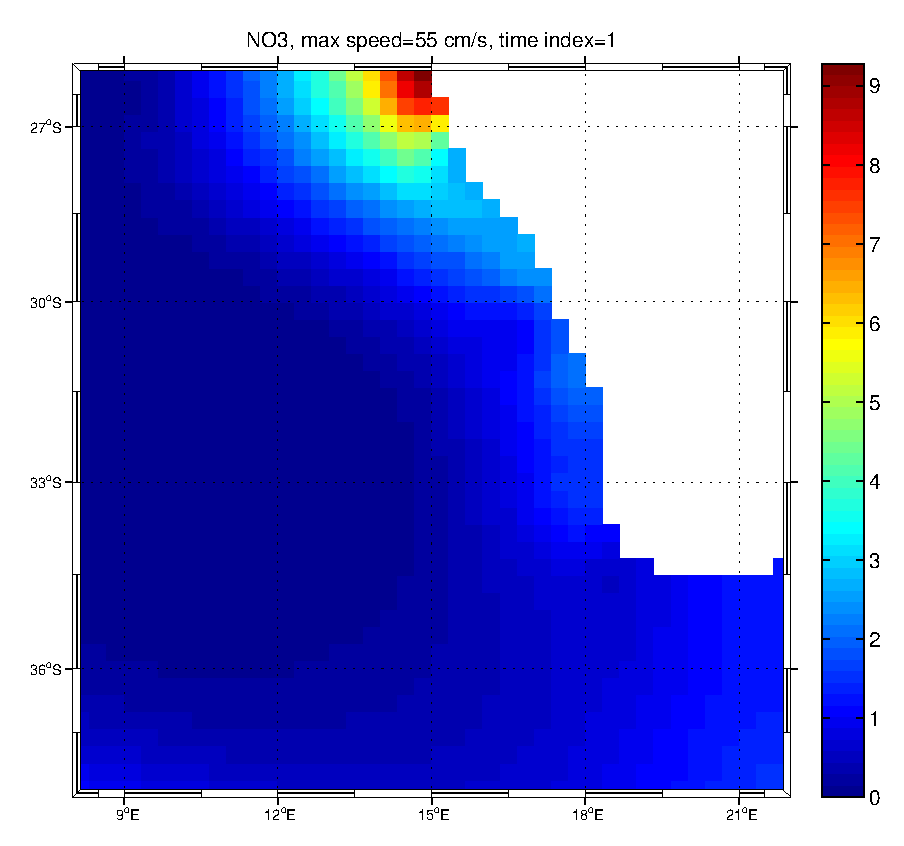
\includegraphics[width=0.4\textwidth]{NO3_surf_t1.eps}}%
\hfill
\subfigure[vertical sections along open boundaries]{
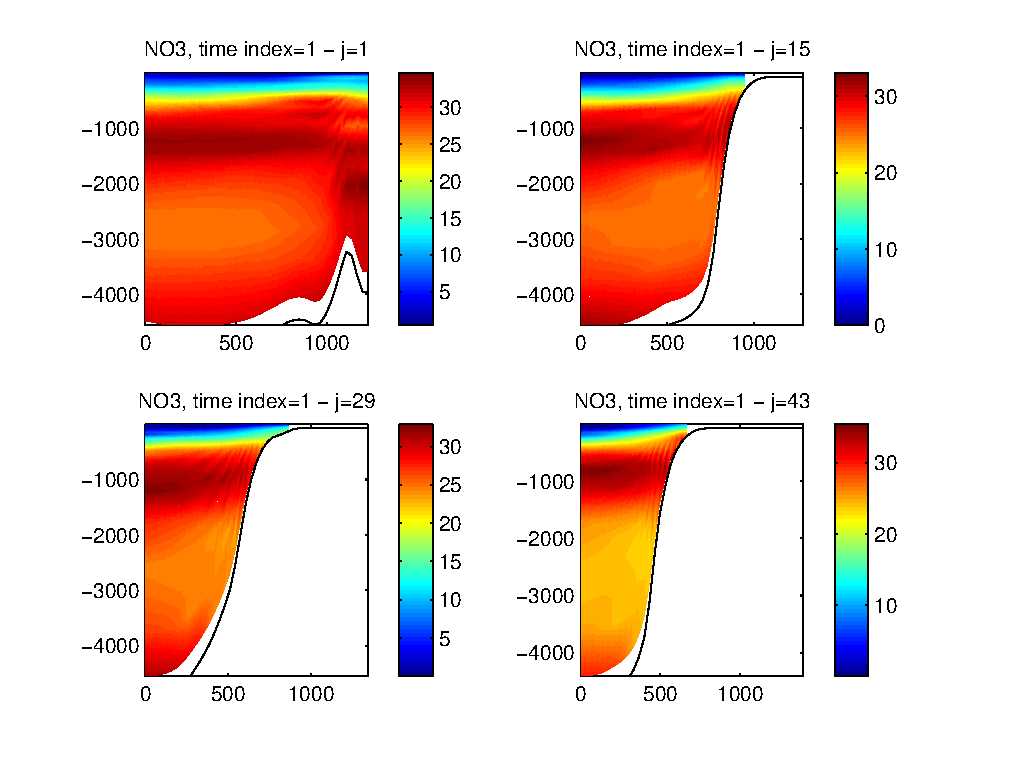
\includegraphics[width=0.70\textwidth]{NO3_profil_t1.eps}}
\caption{Result of make\_clim\_pisces for the Benguela example : NO3 forcing
  fields [mMol N m-3].}
\label{fig:makeclimpiscesNO3}
\end{figure}


\begin{figure}[!htbp]
\subfigure[Surface map]{
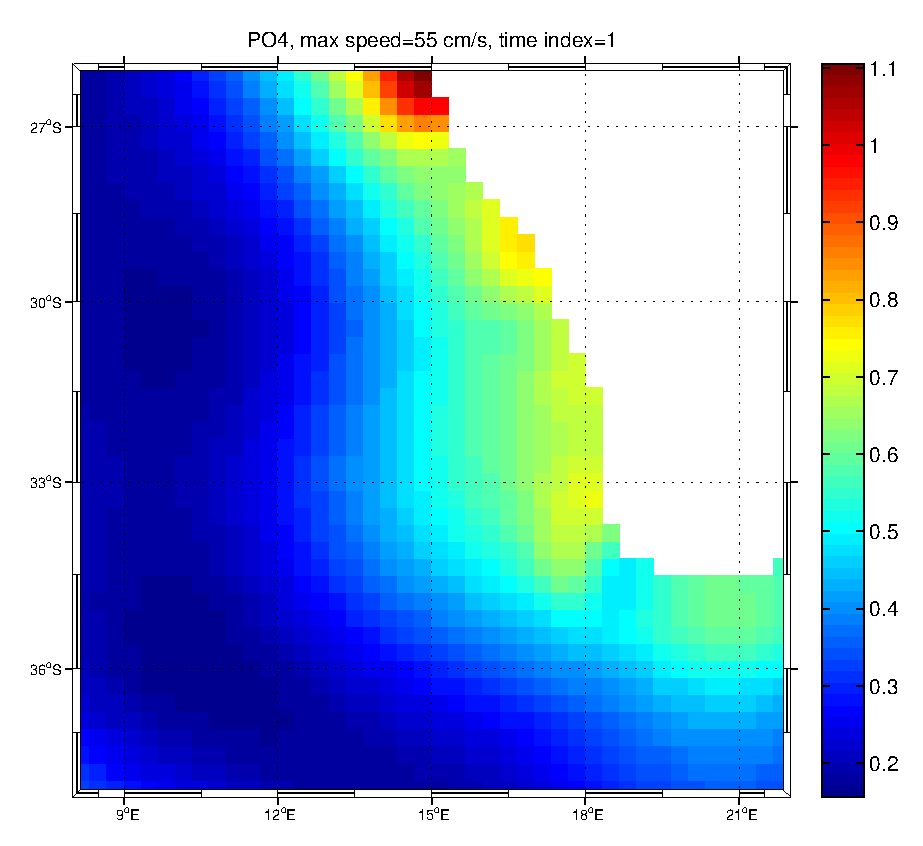
\includegraphics[width=0.4\textwidth]{PO4_surf_t1.eps}}%
\hfill
\subfigure[vertical sections along open boundaries]{
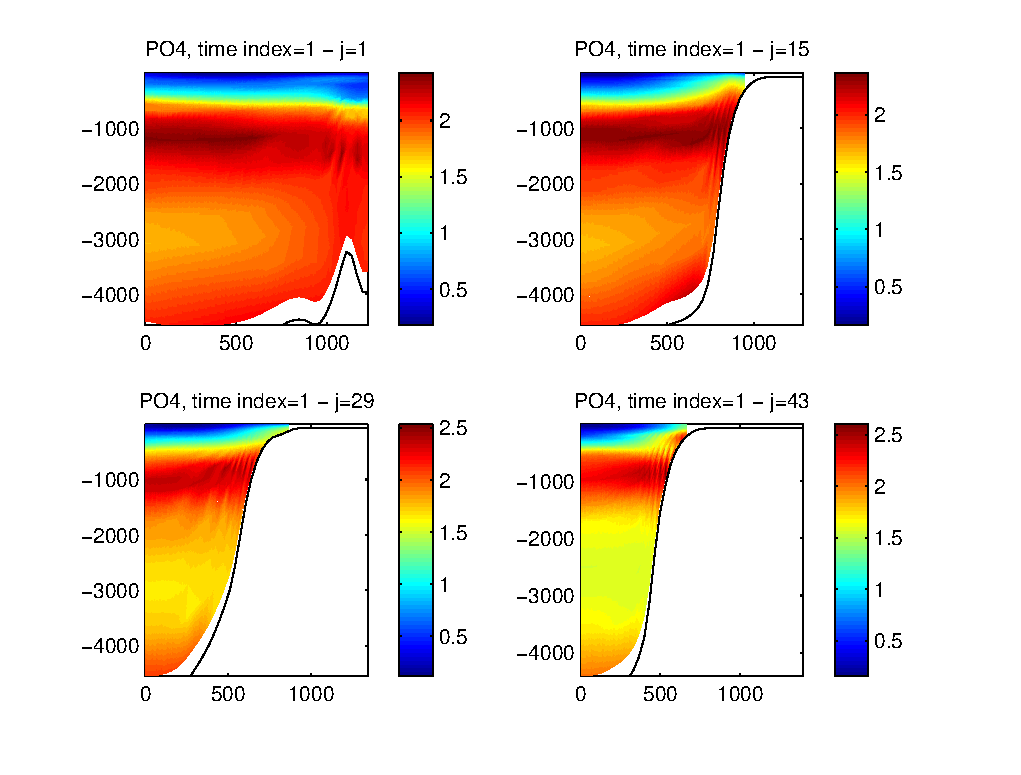
\includegraphics[width=0.70\textwidth]{PO4_profil_t1.eps}}
\caption{Result of make\_clim\_pisces for the Benguela example : PO4 forcing fields
  [mMol P m-3].}
\label{fig:makeclimpiscesNO4}
\end{figure}

\noindent To compute the Iron dust deposition forcing file xxx\_frcbio.nc file :\\
$>>$\\
$>>$ make\_dust\\
\begin{figure}[!htbp]
\centering
\subfigure{
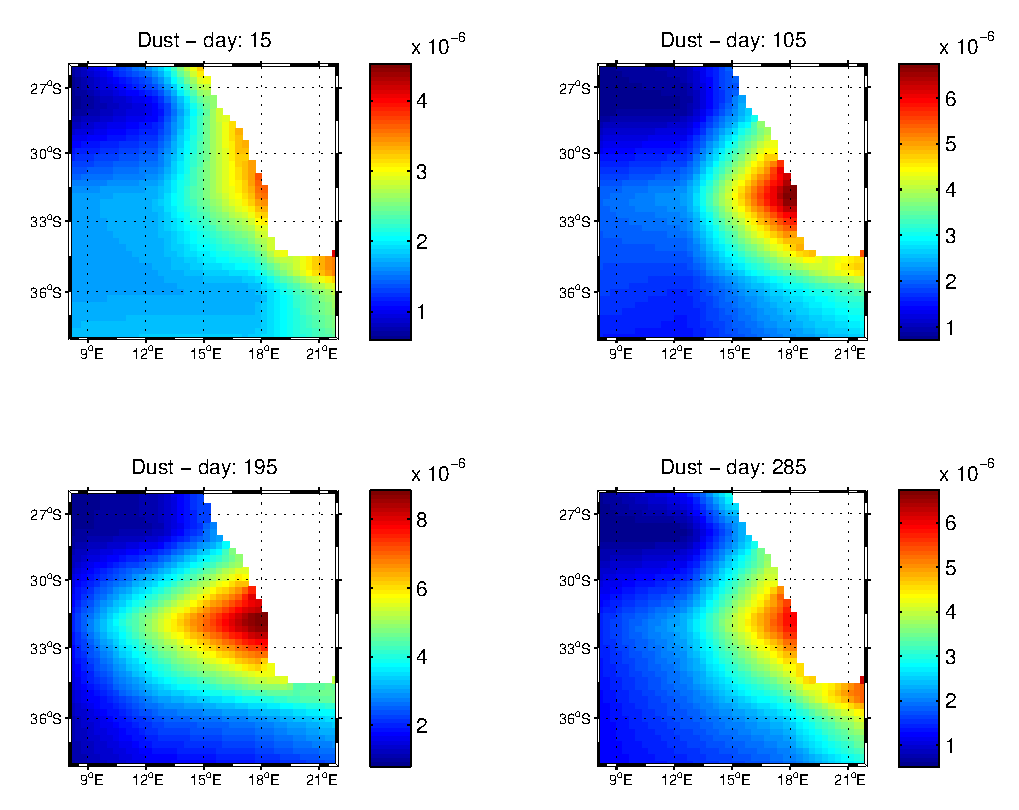
\includegraphics[width=0.8\textwidth]{dustdepo_surface.eps}}%
\hfill
\caption{Result of make\_clim\_pisces for the Benguela example : Iron dust deposition
  forcing fields [nmol Fe m-3].}
\label{fig:makeclimpiscesNO4}
\end{figure}

\section{Inter-Annual simulations}
ROMSTOOLS can help to realize inter-annual simulations. In this context, 
we rely on Ocean Global Circulations Models (OGCM) for the lateral 
boundary conditions and a global atmospheric reanalysis for the surface 
forcing (NCEP). To limit the volume of data which needs to be transfered 
over the Internet, we use Opendap to extract only the necessary subgrids. 

\subsection{Getting the surface forcing data from NCEP}

The Matlab script make\_NCEP.m is used to obtain the surface forcing data.
It downloads the necessary NCEP surface forcing data (Sea Surface 
Temperature, Wind stress ...) over the Internet, and interpolates them on 
the model grid. Since make\_NCEP.m works with the bulk parameterization 
(i.e. the 
BULK\_FLUX and BULK\_EP cpp keys should be defined in cppdefs.h),
a surface forcing NetCDF file and a bulk NetCDF file are generated for 
each month of your simulation in the directory 
$\sim$/Roms\_tools/Run/ROMSFILES/ .
The part of the file romstools\_param.m that you should change is:\\\\
\%\\
\%\%\%\%\%\%\%\%\%\%\%\%\%\%\%\%\%\%\%\%\%\%\%\%\%\%\%\%\%\%\%\%\%\%\%\%\%\%\%\%\%\%\%\%\%\%\%\%\%\%\%\%\%\%\\
\%\\
\% 7 Parameters for Interannual forcing (SODA, ECCO, NCEP, ...)\\
\%\\
\%\%\%\%\%\%\%\%\%\%\%\%\%\%\%\%\%\%\%\%\%\%\%\%\%\%\%\%\%\%\%\%\%\%\%\%\%\%\%\%\%\%\%\%\%\%\%\%\%\%\%\%\%\%\\
\%\\
\% Path to Forcing data\\
\%\\
FORC\_DATA\_DIR = [RUN\_dir,'DATA/'];\\
\%\\
Download\_data = 1;                            \% Get data from the OPENDAP sites \\
level         = 0;                            \% AGRIF level; 0=parent grid \\
\%\\
\%  Options for make\_NCEP\\
\%\\
NCEP\_dir= [FORC\_DATA\_DIR,'NCEP\_',ROMS\_config,'/']; \% NCEP data directory\\
makefrc      = 1;                            \% 1: Create forcing files\\
makeblk      = 1;                            \% 1: Create bulk files\\
add\_tides     = 0;                     \% 1: Add the tides (To be done...)\\
\%\\
NCEP\_version  = 1;                            \% NCEP version:\\
\%                                 (1: NCEP/NCAR Reanalysis, 1/1/1948 - present\\
\%                                  2: NCEP-DOE Reanalysis, 1/1/1979 - 12/31/2001)\\
\%\\
\\
Variables description :
\begin{itemize}
\item FORC\_DATA\_DIR : Directory where the different files downloaded over 
the Internet are stored.
\item Download\_data : Get data from the OPENDAP sites. Should be 1.
\item level : AGRIF level. The parent grid = 0 and the child grid = 1.
\item NCEP\_dir= [FORC\_DATA\_DIR,'NCEP\_',ROMS\_config,'/'] : NCEP data directory. 
This is where NCEP data downloaded over the Internet are stored.
\item makefrc : Switch to define if the forcing file is generated. Should be 1.
\item makeblk : Switch to define if the bulk file is generated. Should be 1.
\item add\_tides : Switch to define if the tidal forcing is added. 
\item NCEP\_version : version of the NCEP reanalysis. 1: NCEP/NCAR Reanalysis, 1/1/1948 - present.
2: NCEP-DOE Reanalysis, 1/1/1979 - 12/31/2001.
\end{itemize}

Save romstools\_param.m and run make\_NCEP in the Matlab session.
You should obtain:
\\\\
$>>$ make\_NCEP\\
Add the paths of the different toolboxes\\
Arch : x86\_64 - Matlab version : 2006a\\
Use of mexnc and loaddap in 64 bits.\\
Download NCEP data with OPENDAP\\
\\
Get NCEP data from 2000 to 2000\\
Minimum Longitude: 12.3\\
Maximum Longitude: 20.3\\
Minimum Latitude: -35.5\\
Maximum Latitude: -26.3815\\
\\
Making output data directory ../Run/DATA/NCEP\_Benguela/\\
Process the first dataset: http://www.cdc.noaa.gov/cgi-bin/nph-nc/Datasets/ncep.reanalysis/surface\_gauss/\\
    Create ../Run/DATA/NCEP\_Benguela/land.sfc.gauss.nc\\
Processing year: 2000\\
  Processing month: 1\\
    Get air for year 2000 - month 1\\
...


\subsection{Getting the surface windstress data from QuickSCAT}
\%\%\%\%\%\%\%\%\%\%\%\%\%\%\%\%\%\%\%\%\%\%\%\%\%\%\%\%\%\%\%\%\%\%\%\%\%\%\%\%\%\%\%\%\%\%\%\%\%\%\%\%\%\%\%\%\%\\
\%\\
\% 7 Parameters for Interannual forcing (SODA, ECCO, NCEP, ...)\\
\%\\
\%\%\%\%\%\%\%\%\%\%\%\%\%\%\%\%\%\%\%\%\%\%\%\%\%\%\%\%\%\%\%\%\%\%\%\%\%\%\%\%\%\%\%\%\%\%\%\%\%\%\%\%\%\%\%\%\%\%\\
\%\\
\% Path to Forcing data\\
.....\\
\%  Options for make\_QSCAT\_daily and make\_QSCAT\_clim\\
\%\\
QSCAT\_dir        = [FORC\_DATA\_DIR,'QSCAT\_',ROMS\_config,'/'];\% QSCAT data directory.\\
QSCAT\_frc\_prefix = [frc\_prefix,'\_QSCAT\_'];                  \% generic forcing file name\\
                                                                 \% for interannual roms simulations with QuickSCAT.\\
QSCAT\_clim\_file  = [DATADIR,'QuikSCAT\_clim/',...              \% QuikSCAT climatology\\
                    'roms\_QSCAT\_month\_clim\_2000\_2007.nc'];       \% file for make\_QSCAT\_clim.\\
\%\\
\%\%\%\%\%\%\%\%\%\%\%\%\%\%\%\%\%\%\%\%\%\%\%\%\%\%\%\%\%\%\%\%\%\%\%\%\%\%\%\%\%\%\%\%\%\%\%\%\%\%\%\%\%\%\%\%\%\%\\

If you want to use the QSCAT daily data, provided by the OpenDAP server at Ifremer,
France: http://www.ifremer.fr/dodsG/CERSAT/quikscat\_daily. \\

$>>$ make\_QSCAT\_daily \\

if you download data over the internet using OpenDAP, you should obtain that during
the dowload step : 

\noindent $>>$ \\ 
...\\ 
Reading: http://www.ifremer.fr/dodsG/CERSAT/quikscat\_daily\\
  Constraint: mwst[167:167][78:113][370:409]\\
Server version: apache-coyote/1.1\\
    Processing day: 1\\
\\
Reading: http://www.ifremer.fr/dodsG/CERSAT/quikscat\_daily\\
  Constraint: zwst[168:168][78:113][370:409]\\
Server version: apache-coyote/1.1\\
\\
Reading: http://www.ifremer.fr/dodsG/CERSAT/quikscat\_daily\\
  Constraint: mwst[168:168][78:113][370:409]\\
Server version: apache-coyote/1.1\\
    Processing day: 2\\
....\\
$>>$\\ 
\\

If you want to use the QSCAT climatology, computed over $2000$-$2007$, based over
these previous QSCAT data :\\

\noindent $>>$ make\_QSCAT\_clim \\
$>>$ ...\\

\subsection{Getting the lateral boundary conditions}

Initial conditions and lateral boundary conditions and  can be 
obtained from several ocean global circulation models (OGCM) 
such as SODA \citep{Car05} or ECCO \citep{Sta99}. The SODA 
reanalysis is available from 1958 to 2001 and ECCO is available 
from 1993 until now. The Matlab script make\_OGCM.m is used to 
download data over the Internet, and to perform the interpolations 
on the model grid. 
A lateral boundary conditions NetCDF file is generated for each month 
of your simulation in the directory $\sim$/Roms\_tools/Run/ROMSFILES/ . 
\\
\\
The part of the file romstools\_param.m that you should change is:
\\
\\
\%\%\%\%\%\%\%\%\%\%\%\%\%\%\%\%\%\%\%\\
\%\\
\% Options for make\_OGCM \\
\%\\
\%\%\%\%\%\%\%\%\%\%\%\%\%\%\%\%\%\%\%\\
OGCM        = 'SODA';                                \% Select the OGCM:
SODA(1958-2001), ECCO(1993-2005), ...\\
OGCM\_dir    = [FORC\_DATA\_DIR,OGCM,'\_',ROMS\_config,'/'];  \\
bry\_prefix  = [ROMS\_files\_dir,'roms\_bry\_',OGCM,'\_']; \\
clm\_prefix  = [ROMS\_files\_dir,'roms\_clm\_',OGCM,'\_']; \\
ini\_prefix  = [ROMS\_files\_dir,'roms\_ini\_',OGCM,'\_']; \\
OGCM\_prefix = [OGCM,'\_'];                            \\
rmdepth     = 2;                                    \\ 
\%                             \\
\%                        \\
\\\\\\
Variables description :
\begin{itemize}
\item OGCM = 'SODA' : Name of the OGCM employed (SODA or ECCO).
\item OGCM\_dir    = [FORC\_DATA\_DIR,OGCM,'\_',ROMS\_config,'/']  : 
OGCM data directory.
\item bry\_prefix  = [ROMS\_files\_dir,'roms\_bry\_',OGCM,'\_'] : 
Left part of the boundary file name.
\item clm\_prefix  = [ROMS\_files\_dir,'roms\_clm\_',OGCM,'\_'] : 
Left part of the climatology file name.
\item ini\_prefix  = [ROMS\_files\_dir,'roms\_ini\_',OGCM,'\_'] : 
Left part of the initial file name.
\item OGCM\_prefix = [OGCM,'\_'] : 
Left part of the OGCM file name. This is where OGCM data are
stored. 
\item rmdepth = 2 : Number of bottom levels to remove.
This is useful when there is no valid data at this level.
For example, if the depth in the ROMS domain is shallower 
than the OGCM depth.
\end{itemize}
Save romstools\_param.m and run make\_OGCM in the Matlab session.
You should obtain:
\\\\
$>>$ make\_OGCM\\
Add the paths of the different toolboxes\\
Arch : x86\_64 - Matlab version : 2006a\\
Use of mexnc and loaddap in 64 bits.\\
Download data...\\
\\
Get data from Y2000M1 to Y2000M3\\
Minimum Longitude: 12.3\\
Maximum Longitude: 20.3\\
Minimum Latitude: -35.5\\
Maximum Latitude: -26.3815\\
\\
Making output data directory ../Run/DATA/SODA\_Benguela/\\
Process the dataset: http://iridl.ldeo.columbia.edu./SOURCES/.CARTON-GIESE/.SODA/.v1p4p3\\
Processing year: 2000\\
  Processing month: 1\\
    Download SODA for 2000 - 1\\
    ...SSH\\
    ...U\\
...

\subsection{Running the model for interannual runs}

Compile the model with jobcomp (and with the 
cpp keys BULK\_FLUX and BULK\_EP defined) and edit 
the input parameter file 
$\sim$/Roms\_tools/Run/roms\_inter.in as for the
climatology experiments. As for the long simulations, a csh script
(run\_roms\_inter.csh) manages the handling of input and output files.
It also changes the number of time steps so each month has the correct
length. This script takes care of leap years. For example Y1996M2 
(February 1996) is 29 days long.

Part to edit in run\_roms\_inter.csh:\\
\\
\#\\
set MODEL=roms\\
set SCRATCHDIR=`pwd`/SCRATCH\\
set INPUTDIR=`pwd`\\
set MSSDIR=`pwd`/ROMS\_FILES\\
set MSSOUT=`pwd`/ROMS\_FILES\\
set CODFILE=roms\\
set AGRIF\_FILE=AGRIF\_FixedGrids.in\\
\#\\
set BULK\_FILES=1\\
set FORCING\_FILES=1\\
set CLIMATOLOGY\_FILES=0\\
set BOUNDARY\_FILES=1\\
\#\\
\# Atmospheric surface forcing dataset (NCEP, GFS,...)\\
\#\\
set ATMOS=NCEP\\
\#\\
\# Oceanic boundary and initial dataset (SODA, ECCO,...)\\
\#\\
set OGCM=SODA\\
\#\\
\# Model time step [seconds]\\
\#\\
set DT=5400\\
\#\\
\# number total of grid levels (1: No child grid)\\
\#\\
set NLEVEL=1\\
\#\\
set NY\_START=2000\\
set NY\_END=2000\\
set NM\_START=1\\
set NM\_END=3\\
\#\\
\#  Restart file - RSTFLAG=0 --$>$ No Restart\\
\#		  RSTFLAG=1 --$>$ Restart\\
\#\\
set RSTFLAG=0\\
\#\\
\#  Time Schedule  -  TIME\_SCHED=0 --$>$ yearly files\\
\#                    TIME\_SCHED=1 --$>$ monthly files\\
\#\\
set TIME\_SCHED=1\\
\#\\
\#\#\#\#\#\#\#\#\#\#\#\#\#\#\#\#\#\#\#\#\#\#\#\#\#\#\#\#\#\#\#\#\#\#\#\#\#\#\#\#\#\#\#\#\#\#\#\#\#\#\#\#\#\#\#\#
\\
\\
Variables definitions:
\begin{itemize}
\item MODEL=roms : Name used for the input files. For example roms\_grd.nc.
\item SCRATCHDIR=`pwd`/SCRATCH : Scratch directory where the model is run.
\item INPUTDIR=`pwd` : Input directory where the roms\_inter.in input file
is located.
\item MSSDIR=`pwd`/ROMS\_FILES : Directory where the roms input NetCDF files
(roms\_grd.nc, roms\_frc.nc, ...) are stored.
\item MSSOUT=`pwd`/ROMS\_FILES : Directory where the roms output NetCDF files
(roms\_his.nc, roms\_avg.nc, ...) are stored.
\item CODFILE=roms : ROMS executable.
\item AGRIF\_FILE=AGRIF\_FixedGrids.in : AGRIF input file which defines the 
position of child grids when using embedding.
\item BULK\_FILES=1 : 1 if using bulk NetCDF files (should be 1 for NCEP).
\item FORCING\_FILES=1 : 1 if using forcing NetCDF files (should be 1 for NCEP).
\item CLIMATOLOGY\_FILES=0 : 1 if using XXX\_clm.nc files. Using a climatology
file for each month can take a lot of disc space. It is less costly to use
 boundary files (XXX\_bry.nc). 
\item BOUNDARY\_FILES=1 : 1 if using XXX\_bry.nc files. 
\item ATMOS=NCEP : name of the atmospheric reanalysis. For the moment it is only
NCEP.
\item OGCM=SODA : name of the OGCM for the boundary conditions. SODA or ECCO.
\item DT=5400 : Model time step in seconds.
\item NDAYS = 30 : Number of days in 1 month.
\item NLEVEL=1 : Total number of model grids (no embedding: NLEVEL=1).
\item NY\_START=2000 : Starting year.
\item NY\_END=2000 : Ending Year.
\item NM\_START=1 : Starting month.
\item NM\_END=3 : Ending month.
\item RSTFLAG=0 : 1 if restarting a simulation
\item TIME\_SCHED=1 : (obsolete) 0 if using yearly files, 1 if using monthly 
files. Since make\_NCEP and make\_OGCM are creating only monthly
files, it should be always 1.
\end{itemize}


As for ROMS long climatology experiments, inter-annual experiments can be run
in batch mode:\\
$>$: nohup ./run\_roms\_inter.csh $>$ exp1.out \&\\\\


\section{Embedding}
%
% nesting
%

\subsection{Introduction}

To address the challenge of bridging the gap between near-shore and
offshore dynamics, a nesting capability has been added to ROMS
and tested for the California Upwelling System \citep{Pen04}.
The method chosen for embedded griding takes advantage of the AGRIF
(Adaptive Grid Refinement in Fortran) package \citep{Bla99,Deb00,
Deb03a,Deb03b}.
AGRIF is a Fortran 95 package for the inclusion of adaptive mesh refinement
features within a finite difference numerical model. One of
the major advantages of AGRIF in static-grid embedding is the ability to
manage an arbitrary number of fixed grids and an arbitrary number of
embedding levels.

\begin{figure}[htbp]
\centerline{\psfig{figure=nesting_fig1.eps,width=15cm}}
\caption{Temporal coupling between a parent and a child grid
for a refinement factor of 3.  The coupling is done at the baroclinic
time step.}
\label{fig:temp_coupling}
\end{figure}

A recursive integration procedure manages the time evolution for the
child grids during the time step of the parent grids
(Figure \ref{fig:temp_coupling}). In order to preserve the CFL 
criterion, for a typical
coefficient of refinement (say, a factor of 3 for a 5 km resolution
grid embedded in a 15 km grid), for each parent time step the child
must be advanced using a time step divided by the coefficient of
refinement as many time as necessary to reach the time of the parent
(Figure (\ref{fig:temp_coupling})).  For simple 2-level embedding, the
procedure is as follows:\\
\begin{enumerate}
\item Advance the parent grid by one parent time step.
\item Interpolate the relevant parent variables in space and time
to get the boundary conditions for the child grid.
\item Advance the child grid by as much child time steps as necessary
to reach the new parent model time.
\item Update point by point the parent model by averaging the more
accurate values of the child model (in the case of 2-way embedding).
\end{enumerate}
The recursive approach used in AGRIF
allows the specification of any number
of embedding level.

\subsection{Embedded (child) model preparation}

To run an embedded model, the user must provide the grid, the surface 
forcing and the initial conditions. To name the different files,
AGRIF employs a specific strategy: if the parent file names are of
the form: XXX.nc, the first child names will be of the form: 
XXX.nc.1, the second: XXX.nc.2, etc... 
This convention is also applied for the "roms.in" input files.

A graphic user interface (NestGUI) facilitates the generation of 
the different NetCDF files. Launch nestgui in the Matlab session 
(in the $\sim$/Roms\_tools/Run/ directory):
\\ \\
$>>$\\
$>>$ nestgui
\\ \\
A window pops up, asking for a "PARENT GRID" NetCDF file 
(Figure \ref{fig:nestgui1}). In our Benguela test case, you should select 
$\sim$/Roms\_tools/Run/ROMSFILES/roms\_grd.nc (grid file) and click "open".
The main window appears (Figure \ref{fig:nestgui2}).

\begin{figure}[!ht]
\centerline{\psfig{figure=nesting_select.eps,width=5cm}}
\caption{Entrance window of NestGUI}
\label{fig:nestgui1}
\end{figure}
 
\begin{figure}[!ht]
\centerline{\psfig{figure=nesting.eps,width=12cm}}
\caption{The NestGUI main window}
\label{fig:nestgui2}
\end{figure}

To generate the child model you should follow several steps:

\begin{enumerate}

\item To define the child domain, click "Define child" and create
the child domain on the main window. The size of the grid child
(Lchild and Mchild) is now visible. This operation can be redone 
until you are satisfied with the size and the position of the child 
domain. The child domain can be finely tuned using the imin, 
imax, jmin and jmax boxes. 
Be aware that the mask interpolation from the parent grid
to the child grid is not optimal close to corners. Parent/Child
boundaries should be placed where the mask is showing a straight
coastline. A warning will be given during the interpolation
procedure if this is not the case.

\item "Interp child" : It generates the child grid file. Before, 
you should select if you are using a new topography
("New child topo" button) for the child
grid or if you are just interpolating the parent topography
on the child grid. In the first case, you should defines
what topography file will be used (e.g. 
$\sim$/Roms\_tools/Topo/etopo2.nc or another dataset).
You should also define if you want the volume of the child grid 
to match the volume of the parent close to the parent/child 
boundaries ("Match volume" button, it should be "on" by default).
You should also define define the r factor \citep{Bec93} 
for topography smoothing ("r-factor", 0.25 is safe) and
the number of points to connect the child topography to the
parent topography ("n-band", it follows the relation 
$h_{new}=\alpha.h_{child} + (1-\alpha).h_{parent}$, 
where $\alpha$ is going from 0 to 1 in "n-band" points 
from the parent/child boundaries).
You should also select the child minimum depth ("Hmin",
it should be lower or equal to the parent minimum depth),
the maximum depth at the coast ("Hmax coast"), the 
number of selective hanning filter passes for the deep 
regions ("n filter deep") and the number of final 
hanning filter passes ("n filter final").

\item "Interp forcing": It interpolates the parent 
surface forcing  on the child grid. Select the parent forcing file
to be interpolated (e.g. $\sim$/Roms\_tools/Run/ROMSFILES/roms\_frc.nc). 
The child forcing file roms\_frc.nc.1 will be created. 
The parent surface fluxes are interpolated on the child grid. 
You can use "Interp bulk" if you are using a bulk formula.
In this case, the parent bulk file 
(e.g. $\sim$/Roms\_tools/Run/ROMSFILES/roms\_blk.nc) will be
interpolated on the child grid.

\item "Interp initial": It interpolates parent initial
conditions on the child grid. Select the parent initial file
(e.g. $\sim$/Roms\_tools/Run/ROMSFILES/roms\_ini.nc).
The child initial file 
(e.g. $\sim$/Roms\_tools/Run/ROMSFILES/roms\_ini.nc.1) 
will be created.
If the topographies are different between the parent and 
the child grids, the child initial conditions are 
vertically re-interpolated. In this case you should check 
if the options "vertical corrections" and "extrapolations"
are selected.
"Interp biology" can be used to interpolate
parent biological variables for biogeochemical experiments.
"Interp restart" generates a child restart file from 
a parent restart file 
(e.g. $\sim$/Roms\_tools/Run/ROMSFILES/roms\_rst.nc). 
This can be done to "hot start" a child model after the 
spin-up of the parent model.

\item You can click on "Create roms.in.*" to generate a
child input file (roms.in.1) from the parent input
file and click on "Create AGRIF\_FixedGrids.in" to 
generate a AGRIF\_FixedGrids.in file (the file which
defines the child grid position in the parent grid).

\end{enumerate}

"river" can be used to locate the river on the coast.
"Interp clim" can be useful to generate boundary conditions 
to test the child model alone. 

\subsection{Compiling and running the model}

The ROMS nesting procedure needs a Fortran 95 compiler. For Linux PCs,
the Intel Fortran Compiler (ifort) is available at \\
http://www.intel.com/software/products/compilers/flin/noncom.htm.
To be able to compile ROMS with ifort, you should change the corresponding 
comments in jobcomp. Define AGRIF in \\
$\sim$/Roms\_tools/Run/cppdefs.h.
Other cpp keys are related to AGRIF:
\begin{itemize}
\item AGRIF\_OBC\_EAST : Open eastern boundary for the child grids.
\item AGRIF\_OBC\_WEST : Open western boundary for the child grids.
\item AGRIF\_OBC\_SOUTH : Open southern boundary for the child grids.
\item AGRIF\_OBC\_NORTH : Open northern boundary for the child grids.
\item AGRIF\_STORE\_BAROT\_CHILD : Store ubar and vbar during the parent step for the
child boundary conditions.
\item AGRIF\_FLUX\_BC : Apply parent/child barotropic boundary conditions has 
fluxes.
\item AGRIF\_POLY\_DUAVG : Apply a third order polynomial temporal interpolation 
for DU\_avg1 and DU\_avg2.
\item AGRIF\_LOCAL\_VOLCONS : Enforce parent-child mass conservation.
\item AGRIF\_OBC\_M2FLATHER :  Activate Flather open boundary conditions for ubar and vbar
for the child model .
\item AGRIF\_OBC\_M2ORLANSKI : Activate 2D radiation open boundary conditions for ubar and vbar
for the child model.
\item AGRIF\_OBC\_M2SPECIFIED : Activate specified open boundary conditions for ubar and vbar
for the child model.
\item AGRIF\_OBC\_M2CHARACT :  Activate open boundary conditions based on characteristic methods 
for ubar and vbar
for the child model.
\item AGRIF\_OBC\_M3ORLANSKI : Activate 2D radiation open boundary conditions for u and v
for the child model.
\item AGRIF\_OBC\_M3SPECIFIED : Activate specified open boundary conditions for u and v
for the child model.
\item AGRIF\_OBC\_M3CHARACT : Activate open boundary conditions based on characteristic methods 
for u and v
for the child model.
\item AGRIF\_OBC\_TORLANSKI :  Activate 2D radiation open boundary conditions for tracers
for the child model .
\item AGRIF\_OBC\_TUPWIND : Activate upwind open boundary conditions for tracers
for the child model.
\item AGRIF\_OBC\_TSPECIFIED  : Activate specified open boundary conditions for tracers
for the child model.
\end{itemize}
The default definitions should be sufficient for most of the applications.
\\
\\
It is possible to edit the file AGRIF\_FixedGrids.in. 
This file contains the child grid positions
(i.e. imin,imax,jmin,jmax) and coefficients of refinement. A first line
gives the number of children grids per parent (if AGRIF\_STORE\_BAROT\_CHILD
is defined, only one child grid can be defined per parent grid). A second
line gives the relative position of each grid and the coefficient of refinement 
for each dimension. 
Edit the input files roms.in.1, roms.in.2 , etc... to define correctly the 
file names and the time steps. To run the model, simply type at the prompt:
roms roms.in.

To visualize the ROMS model outputs for different grid levels, 
change the value in the "child models" box
in roms\_gui.




\newpage
\section{Operational coastal modeling system}
An operating coastal modeling system can be designed following the 
assumption that large scale offshore dynamics are slow in comparison 
to the coastal system. The lateral boundary conditions are interpolated 
from the last available ECCO model outputs and are kept constant during
the ROMS simulation. ECCO model outputs are delayed by about two to four 
weeks, but we suppose that they are still relevant for the present large 
scale oceanic structure. The Global Forecast System (GFS) is used for the 
surface forcing. A first day of simulation is run in hindcast mode. This 
will provide the initial conditions for the next simulated day. 
Using GFS as surface forcing and ECCO for the lateral boundary conditions, 
a forecast of 7 days is conducted. A UNIX C-Shell script 
(~/Roms\_tools/Run/run\_roms\_forecast.csh) manages
data downloading, the hindcast and forecast simulations
and datas storage.
The script run\_roms\_forecast.csh starts Matlab in 
batch mode to download
with OPENDAP the lateral boundary conditions from ECCO and 
the surface forcing from GFS. It interpolates the data on ROMS 
grid and launches the hindcast and the forecast runs.

The script run\_roms\_forecast.csh should be edited to change the
directory pathways (HOME, RUNDIR, PATH, LD\_LIBRAIRY\_PATH, MATLAB,...).

The ROMS input files $\sim$/Roms\_tools/Run/roms\_hindcast.in and 
$\sim$/Roms\_tools/Run/roms\_forecast.in should also be edited to change
the length of the time step and the number of time steps. 
The ROMS input file roms\_hindcast.in should be defined such as 
the hindcast run duration
is 1 day and a restart file is generated at the end of the hindcast run.

The script run\_roms\_forecast.csh can be relaunched everyday in batch mode 
using crontab.




\chapter{ROMS\_AGRIF v2.1}
\section{The ROMS model}

ROMS solves the primitive equations in an Earth-centered rotating environment, based
on the Boussinesq approximation and hydrostatic vertical momentum balance. ROMS is
discretized in coastline- and terrain-following curvilinear coordinates.  ROMS is a
split-explicit, free-surface ocean model, where short time steps are used to advance
the surface elevation and barotropic momentum, with a much larger time step used for
temperature, salinity, and baroclinic momentum.  ROMS employs a special 2-way
time-averaging procedure for the barotropic mode, which satisfies the 3D continuity
equation \citep{Shc03b}.  The specially designed predictor-corrector time step
algorithm used in ROMS allows a substantial increase in the permissible time-step
size.

ROMS has been designed to be optimized on shared memory parallel computer
architectures such as the SGI/CRAY Origin 2000. Parallelization is done by two
dimensional sub-domains partitioning. Multiple sub-domains can be assigned to each
processor in order to optimize the use of processor cache memory. This allow
super-linear scaling when performance growth even faster than the number of CPUs.

The third-order, upstream-biased advection scheme implemented in ROMS allows the
generation of steep gradients, enhancing the effective resolution of the solution for
a given grid size \citep{Shc98}. Explicit lateral viscosity is null everywhere in the
model domain except in sponge layers near the open boundaries where it increases
smoothly close to the lateral open boundaries.

A non-local, K-profile planetary (KPP) boundary layer scheme \citep{Lar94}
parameterizes the unresolved physical vertical subgrid-scale processes.  If a lateral
boundary faces the open ocean, an active, implicit, upstream biased, radiation
condition connects the
model solution to the surroundings \citep{Mar01}. \\

%------------------------------------------------------------------------
More informations and model description can also be found in the SCRUM Manuel
\citep{hedstroem97} and a more recent User Manual on ROMS (Rutgers
version\footnote{http://myroms.org}), both written by Kate Hedstr�m\footnote{Kate
  Hedstr�m, University of Alaska Fairbanks, Center for Arctic Region Supercomputing
  Center, University of Alaska Fairbanks, } \citep{hedstroem2009} \footnote{Many
  thanks to Kate Hedstro�m for this work.}. These documents are available on the
ROMS\_AGRIF web site : http://roms.mpl.ird.fr in the documentation section.

%------------------------------
\newpage
\section{Nesting capabilities, 1-WAYS and 2-WAYS using the AGRIF procedure}

\subsection{Introduction}
\label{sec:introduction}

To address the challenge of bridging the gap between near-shore and offshore
dynamics, a nesting capability has been added to ROMS and tested for the California
Upwelling System \citep{Pen04}.  The method chosen for embedded griding takes
advantage of the AGRIF (Adaptive Grid Refinement in Fortran) package
\citep{Bla99,Deb00, Deb03a,Deb03b,Deb08}.  AGRIF is a Fortran 95 package for the
inclusion of adaptive mesh refinement features within a finite difference numerical
model. One of the major advantages of AGRIF in static-grid embedding is the ability
to manage an arbitrary number of fixed grids and an arbitrary number of embedding
levels.

\begin{figure}[htbp]
\centerline{\psfig{figure=nesting_fig1.eps,width=15cm}}
\caption{Temporal coupling between a parent and a child grid for a refinement factor
  of 3.  The coupling is done at the baroclinic time step.}
\label{fig:temp_coupling}
\end{figure}

A recursive integration procedure manages the time evolution for the child grids
during the time step of the parent grids (Figure \ref{fig:temp_coupling}). In order
to preserve the CFL criterion, for a typical coefficient of refinement (say, a factor
of 3 for a 5 km resolution grid embedded in a 15 km grid), for each parent time step
the child must be advanced using a time step divided by the coefficient of refinement
as many time as necessary to reach the time of the parent (Figure
(\ref{fig:temp_coupling})).  For simple 2-level embedding, the
procedure is as follows:\\
\begin{enumerate}
\item Advance the parent grid by one parent time step.
\item Interpolate the relevant parent variables in space and time to get the boundary
  conditions for the child grid.
\item Advance the child grid by as much child time steps as necessary
to reach the new parent model time.
\item Update point by point the parent model by averaging the more accurate values of
  the child model (in the case of 2-way embedding).
\end{enumerate}
The recursive approach used in AGRIF allows the specification of any number of
embedding level. Other cpp keys are related to AGRIF, they are in
  set\_global\_definitions.h and set\_obc\_definitions.h files. These ones are the
  default conditions, are located in the ROMS\_AGRIF code sources and should not be
  edit by standard user.

\subsection{2-WAYS nesting:  feed-back from child to parent grid}
\label{sec:2-ways-nesting}
\textbf{To be continued ...}


% \subsection{Specification in the ROMS\_AGRIF $2.0$ code}\label{sec:spec_romsagrif2.0}
% Here are the main cpp-keys related to AGRIF nesting procedure.
% \begin{itemize}
% \item AGRIF\_OBC\_EAST : Open eastern boundary for the child grids.
% \item AGRIF\_OBC\_WEST : Open western boundary for the child grids.
% \item AGRIF\_OBC\_SOUTH : Open southern boundary for the child grids.
% \item AGRIF\_OBC\_NORTH : Open northern boundary for the child grids.
% \item AGRIF\_FLUX\_BC : Apply parent/child barotropic boundary conditions as fluxes.
% \item AGRIF\_OBC\_M2FLATHER :  Activate Flather open boundary conditions for ubar and vbar
% for the child model .
% \item AGRIF\_OBC\_M2ORLANSKI : Activate 2D radiation open boundary conditions for ubar and vbar
% for the child model.
% \item AGRIF\_OBC\_M2SPECIFIED : Activate specified open boundary conditions for ubar and vbar
% for the child model.
% \item AGRIF\_OBC\_M2CHARACT : Activate open boundary conditions based on
%   characteristic methods for ubar and vbar for the child model.
% \item AGRIF\_OBC\_M3ORLANSKI : Activate 2D radiation open boundary conditions for u and v
% for the child model.
% \item AGRIF\_OBC\_M3SPECIFIED : Activate specified open boundary conditions for u and v
% for the child model.
% \item AGRIF\_OBC\_M3CHARACT : Activate open boundary conditions based on characteristic methods 
% for u and v for the child model.
% \item AGRIF\_OBC\_TORLANSKI :  Activate 2D radiation open boundary conditions for tracers
% for the child model .
% \item AGRIF\_OBC\_TUPWIND : Activate upwind open boundary conditions for tracers
% for the child model.
% \item AGRIF\_OBC\_TSPECIFIED  : Activate specified open boundary conditions for tracers
% for the child model.
% \end{itemize}

% \begin{center}
%   \bf The default definitions should be sufficient for most of the applications.
%\end{center}
%------------------------------
\section{Changelog since ROMS\_AGRIF 1.1} \label{changelog}
\begin{itemize}
\item \underline{New diffusive-advection schemes} : RSUP3 \citep{Marches09} \\

  To avoid unacceptable spurious diapycnal mixing, a new advection scheme has been
  proposed and validate : the RSUP3 scheme. The diffusion is split from advection and
  is represented by a rotated biharmonic diffusion scheme with flow-dependent
  hyperdiffusivity satisfying the Peclet constraint. The rotated diffusion operator
  is designed for numerical stability, which includes improvements of linear
  stability limits and a clipping method adapted to the sigma-coordinate.

  This scheme induce a time step smaller than the third-order upstream biaised
  diffusive advective scheme used in the version $1.0$. It is activated by the use of
  the cppkeys \textbf{TS\_SPLIT\_UP3} for tracers and \textbf{UV\_SPLIT\_UP3} for
  momentum in the cppdefs.h file.

  To avoid numerical instabilities in the sponge where there is enhanced
  diffusion/diffsuivity, a classical laplacian diffusion can be applied by the use of
  the cppkey \textbf{SPONGE\_DIF2} and \textbf{SPONGE\_VIS2} in the cppdefs.h file.





\item \underline{Two-ways AGRIF nesting} : Ref \citep{Debreu09-1, Debreu09-2} \\

  As presented before, it is the capability of the fine grid to update data in the
  coarse grid. With this procedure, we are now able to get the impact of high
  resolution on the more coarser reolution, in a context of upscaling.  To activate
  the two ways nesting, you need to define the \textbf{AGRIF} and
  \textbf{AGRIF\_2WAY} cpp-keys.


\item \underline{Bulk formulation} : \\
Desciption of the bulk formulation coded by Patrick.


\item \underline{Online diagnostics and I/O}: \\

  New diagnostics and outputs are now available in the ROMS\_AGRIF $2.0$.  

  Wind stresses, windspeed, and heat fluxes (latent, sensible, long-wave and solar
  short wave) can be written in the netCDF history and average files. Moreover,
  bottom boundary layer thickness and euphotic depth layer in case of biological
  experiments can be saved. For more information, you can refer at the section
  \ref{namelistdesc}.

  Improvmement have also been carried out on the tracer and momentum equation term
  diagnostics.  

  From now, the tracer equation terms are in \textit{dia.nc} and \textit{dia\_avg.nc}
  netcdf file with flags that permit to choose exactly the term
  you want to write in the NetCDF files.\\
  By default this diagnostics are written in a divergence flux form, ($\partial{u
    T}_{x}$, $\partial{v T}_{y}$, ...) but they can be written in an "advective form"
  : $u\partial{T}_{x}$, $v
  \partial{T}_{y}$, ... by using the \textbf{DIAGNOSTICS\_TS\_ADV} cpp key.
  Some term have been added : the term integrated over the mixed layer depth (cppkeys
  \textbf{DIAGNOSTICS\_TS\_MLD}. The mixed layer depth is computed online, from the
  closure module.
\\ \\
The differents term of the tracer equation, that can be diagnose,
for each tracer,  expressed in $C^{o}.s^{-1}$ ,  are:
  \begin{itemize}
   \item Time evolution term (called "rate" term)
   \item Zonal advective term
   \item Meridian advective term
  �\item Vertical advective term
   \item Horizontal mixing term
   \item Vertical mixing term
   \item Nudging $+$ Surface forcing term (called Tforc term) 
   \item In the case of use \textbf{DIAGNOSTICS\_TS\_MLD} some additional terms are
     diagnosted :
     \begin{itemize}
     \item Time evolution term integrated over the surface mixed layer depth (MLD hereafter)
     \item Zonal advective term integrated over the MLD
     \item Meridian advective term integrated over the MLD
    �\item Vertical advective term integrated over the MLD
     \item Horizontal mixing term integrated over the MLD
     \item Vertical mixing term integrated over the MLD
     \item Nudging $+$ Surface forcing term integrated over the MLD
     \item Entrainement term at the base of the mixed layer
     \end{itemize}
  \end{itemize}


  Concerning the momentum equation term, the differents term of the equation can be
  saved in history \textit{diaM.nc} and average \textit{diaM\_avg.nc} netCDF files.
  As the tracer, there are flags to choose exactly the term you want to write in the
  netCDF file. \\

  The differents terms of the momentum equation, expressed in $m.s^{-2}$, that can be diagnose (for u and v)
  are :
  \begin{itemize}
   \item Time evolution term (called "rate" term)
   \item Pressure gradient term
   \item Coriolis term
  �\item Zonal advective
   \item Meridian advective
   \item Vertical advective
   \item Horizontal mixing
   \item Vertical mixing
  \end{itemize}


\end{itemize}







\newpage
\section{Parameters description : \textit{parameter.h}}\label{paramdesc}

In this section, we present the more important parameters to configure your own
roms\_agrif $2.0$ run. These parameters are : 
\begin{itemize}
\item \textbf{Test case or realistic run}: \\
...  \\
\#if defined BASIN $----->$ {\color{red}\textbf{\textit{Test case}}} \\
      parameter (LLm0$=60$,  MMm0$=50$,  N$=10$) \\
\#elif defined REGIONAL $----->$ {\color{red}\textbf{\textit{Realistic run}}} \\
\#$~~$  elif defined  BENGUELA\_LR \\
$~~~~~$      parameter (LLm0$=41$, MMm0$=42$,  N$=32$)  $!$ $<--$ BENGUELA\_LR \\
\#$~~$  else \\ 
$~~~~~$      parameter (LLm0=$39$,  MMm0$=32$,  N$=20$) \\
\#$~~$  endif \\
... \\
LLm0  
MMm0
N

\item \textbf{Grid size}:
  \begin{itemize}
\item LLm0: Dimension (ghost points included) in  the $\xi$ direction.
\item MMm0: Dimension (ghost points included) in  the $\eta$ direction.
\item N: Number of $\rho$-vertical points, in the vertical grid.
  \end{itemize}


\item \textbf{Parallelization}: \\
....\\
$!$ \\
$!$ Domain subdivision parameters: \\
$!$ ====== =========== =========== \\
$!$ NPP            Maximum allowed number of parallel threads; \\
$!$ NSUB\_X,NSUB\_E  Number of SHARED memory subdomains in XI- and \\
$!$                                                ETA-directions; \\
$!$ NNODES        Total number of MPI processes (nodes); \\
$!$ NP\_XI,NP\_ETA  Number of MPI subdomains in XI- and ETA-directions; \\
$!$ \\

AUTOTLING : cppkeys that enable to compute the optimum subdomains partition in terms
of computation time. This is computed during the 100 first time step of the Run
(implemented by Laurent Debreu).

\item \textbf{Tides}: \\
...�\\
\#if defined SSH\_TIDES || defined UV\_TIDES \\
$~~~~~~~~~$      integer Ntides$~~~~~$    \\
$~~~~~~~~~$      parameter (Ntides=8)$--->$ {\color{red}\textit{\textbf{Number of wave in
    the total tidal signal}}} \\
\#endif \\ 
... \\

\end{itemize}
%------------------------------
\newpage
\section{CPP-keys description \textit{cppdefs.h}} \label{cppkeydesc} 


In this section, we present the differents cpp keys used to define the numerical or
physical options in ROMS\_AGRIF. These latters are ordered in differents sections and
described in Table \ref{tab:cppkeys1}.
%------------------------------

\begin{longtable}
   {|p{0.5\linewidth}|p{0.5\linewidth}|}
   \hline
    TYPE & CPP KEYS NAME \\ 
   \endfirsthead
   \hline
   TYPE & CPP KEYS NAME \\ 
   \hline
   \endhead
   \hline
   \multicolumn{2}{|p{0.6666\linewidth}|}{\textit{Next page}$\rightarrow$} \\
   \hline
   \endfoot 
%    \hline \\
% %    \multicolumn{2}{|p{0.6666\linewidth}|}{C'est fini} \\
%    \hline
   \endlastfoot 
\hline

%-------------------------------------------
                 &                      \\
\underline{TEST CASE}      &                      \\
                 &        BASIN           \\
                 &        CANYON\_A       \\
                 &        CANYON\_B       \\
                 &        GRAV\_ADJ       \\
                 &        INNERSHELF      \\
                 &        OVERFLOW        \\
                 &        SEAMOUNT        \\
                 &        SHELFRONT       \\
                 &        SOLITON         \\
                 &        UPWELLING       \\
                 &        INTERNAL        \\
                 &        VORTEX          \\
                 &        REGIONAL : realistric configuration   \\
%------------------------------------------
\hline
\multicolumn{2}{|p{1\linewidth}|}{\centering Basic options} \\
\hline

Configuration Name &                \\
&  BENGUELA \\


Parallelization    &                      \\
                   &    OPENMP            \\
                   &    MPI               \\
& PARALLEL\_FILES \\
& AUTOTILING     \\




Embedding          &                      \\
                   &         AGRIF        \\
                   &         AGRIF\_2WAY  \\


Open Boundary Conditions  &                \\
 &  TIDES                     \\
 &  OBC\_EAST                 \\
 &  OBC\_WEST                 \\
 &  OBC\_NORTH                \\
 &  OBC\_SOUTH                \\


Tides &                \\
& TIDES      \\
& SSH\_TIDES  \\
& UV\_TIDES   \\
& TIDERAMP   \\


Applications          &                     \\
&    BIOLOGY              \\
&    FLOATS               \\
&    STATIONS             \\
&    PASSIVE\_TRACER      \\
&    SEDIMENT  \\
&    BBL  \\
& \\
\hline
\multicolumn{2}{|p{1\linewidth}|}{\centering More advanced options} \\
\hline
Model dynamics         &                      \\
&  SOLVE3D                    \\
&  UV\_COR                     \\
&  UV\_ADV                     \\

Grid configuration     &                      \\
&    CURVGRID          \\
&    SPHERICAL         \\
&    MASKING            \\

Input/Output and Diagnostics     &               \\
&     AVERAGES                  \\
&     AVERAGES\_K                \\
&     DIAGNOSTICS\_TS            \\
&     DIAGNOSTICS\_TS\_ADV        \\
&     DIAGNOSTICS\_TS\_MLD        \\
&     DIAGNOSTICS\_UV \\
    
Equation of State      &                      \\
&                        SALINITY  \\
&                        NONLIN\_EOS  \\
&                        SPLIT\_EOS  \\

Surface Forcing     &                      \\
&                        QCORRECTION \\
&                        SFLX\_CORR \\
&                        DIURNAL\_SRFLUX \\
&                        BULK\_FLUX \\
&                        LW\_ONLINE \\
&                        BULK\_EP \\
&                        BULK\_SMFLUX \\
&                        BULK\_WVEC \\
&                        BULK\_WSTR \\

Lateral Tracer Mixing     &                      \\
&                       MIX\_GP\_TS \\
&                       MIX\_S\_TS \\
&                       MIX\_EN\_TS \\
&                       TS\_DIF2 \\
&                       TS\_DIF4 \\
&                       TS\_SPLIT\_UP3 \\

Lateral Momentum Mixing     &                      \\
&                        MIX\_GP\_UV \\
&                        MIX\_S\_GP \\
&                        UV\_VIS2 \\
&                        UV\_VIS4 \\
&                        UV\_SPLIT\_UP3 \\

Sponge Layer     &                      \\
&                        SPONGE \\


Lateral Forcing  &                      \\ 
 &                      \\ 
\textit{1-Climatology strategy : 3D fields covering the  whole domain }  &           \\
&                        CLIMATOLOGY \\
&                        ZCLIMATOLOGY \\
&                        M2CLIMATOLOGY \\
&                        M3CLIMATOLOGY \\
&                        TCLIMATOLOGY \\
& \\
\textit{2-Boundary strategy : 1D fields only on OBC points} &       \\
&                        FRC\_BRY \\
&                        Z\_FRC\_BRY \\
&                        M2\_FRC\_BRY \\
&                        M3\_FRC\_BRY \\
&                        T\_FRC\_BRY \\


Nudging         &                      \\
&                        ZNUDGING \\
&                        M2NUDGING \\
&                        M3NUDGING \\
&                        TNUDGING \\
&                        ROBUST\_DIAG \\

Bottom Forcing     &                     \\
&                        ANA\_BSFLUX \\
&                        ANA\_BTFLUX \\

Point Sources - Rivers     &                      \\
&                        PSOURCE \\
&                        ANA\_PSOURCE  \\


Vertical Mixing      &                      \\
&                     BODYFORCE  \\
&                     BVF\_MIXING  \\
&                     LMD\_MIXING  \\
&                     LMD\_SKPP  \\
&                     LMD\_BKPP  \\
&                     LMD\_RIMIX  \\
&                     LMD\_CONVEC  \\
&                     LMD\_DDMIX  \\
&                     LMD\_NONLOCAL  \\

Open Boundary Conditions     &                      \\
&                        OBC\_M2SPECIFIED \\
&                        OBC\_M2FLATHER \\
&                        OBC\_M2CHARACT \\
&                        OBC\_M2ORLANSKI \\
&                        OBC\_M2ORLANSKI \\
&                        OBC\_VOLCONS \\
&                        OBC\_M3ORLANSKI \\
&                        OBC\_TORLANSKI \\
&                        OBC\_M3SPECIFIED \\
&                        OBC\_TSPECIFIED \\
%-------------------------------------------
\hline

%--------------------------------------------------------------
\caption{Description of the CPP keys used in the cppdefs.h file}
\label{tab:cppkeys1}
\end{longtable}

\subsection*{Test Case}

\begin{longtable}
   {|p{0.2\linewidth}|p{0.8\linewidth}|}
   \hline
    CPP KEYS NAME & Description \\ 
   \endfirsthead
   \hline
    CPP KEYS NAME  & Description \\ 
   \hline
   \endhead
   \hline
   \multicolumn{2}{|p{0.6666\linewidth}|}{\textit{Next page}$\rightarrow$} \\
   \hline
   \endfoot 

   \endlastfoot 
\hline
%-------------------------------------------
BASIN & Must be defined for running the Basin Example.   \\
CANYON\_A & Must be defined for running the Canyon\_A Example.   \\
CANYON\_B  & Must be defined for running the Canyon\_B Example.    \\
GRAV\_ADJ & Must be defined for running the Gravitational Adjustment Example.   \\
INNERSHELF & Must be defined for running the Inner Shelf Example.   \\
OVERFLOW & Must be defined for running the Gravitational/Overflow Example.   \\
SEAMOUNT & Must be defined for running the Seamount Example.   \\
SHELFRONT & Must be defined for running the Shelf Front Example.     \\
SOLITON &  Must be defined for running the Equatorial Rossby Wave Example.  \\
UPWELLING & Must be defined for running the Upwelling Example.   \\
INTERNAL &  Must be defined for running the Internal tides example.  \\
VORTEX & Must be defined for running the Baroclinic Vortex Example.   \\
REGIONAL & Must be defined if running realistic regional simulations.   \\



%-------------------------------------------
\hline

\caption{Test Case related CPP keys}
\label{tab:cppkeysTestCase}
\end{longtable}

\subsection*{Parallelization}

\begin{longtable}
   {|p{0.25\linewidth}|p{0.75\linewidth}|}
   \hline
    CPP KEYS NAME & Description \\ 
   \endfirsthead
   \hline
    CPP KEYS NAME  & Description \\ 
   \hline
   \endhead
   \hline
   \multicolumn{2}{|p{0.6666\linewidth}|}{\textit{Next page}$\rightarrow$} \\
   \hline
   \endfoot 

   \endlastfoot 
\hline
%-------------------------------------------
OPENMP & Activate the Open-MP parallelization protocol.      \\
MPI & Activate the MPI parallelization protocol.   \\
PARALLEL\_FILES & Activate the I/O writing on multiprocessor.    \\
AUTOTILING & Activate the subdomains partitionning optimization.    \\
%-------------------------------------------
\hline
\caption{Parallelization related CPP keys}
\label{tab:cppkeysparallelization}
\end{longtable}

\paragraph{Preselected options }�\\
\noindent
\# ifdef MPI \\
\# $~$$~$undef PARALLEL\_FILES \\
\# endif \\
\# undef AUTOTILING \\


\subsection*{Embedding}
\begin{longtable}
   {|p{0.2\linewidth}|p{0.8\linewidth}|}
   \hline
    CPP KEY NAME & Description \\ 
   \endfirsthead
   \hline
    CPP KEY NAME  & Description \\ 
   \hline
   \endhead
   \hline
   \multicolumn{2}{|p{0.6666\linewidth}|}{\textit{Next page}$\rightarrow$} \\
   \hline
   \endfoot 

   \endlastfoot 
\hline
%-------------------------------------------
AGRIF & Activate the (1-WAYS) nesting capabilities.   \\
AGRIF\_2WAYS & Add the the 2-WAYS nesting (feedback from child to parent grid) capabilities.   \\
%-------------------------------------------
\hline

\caption{Embedding related CPP keys}
\label{tab:cppkeyNesting}
\end{longtable}

\subsection*{Open Boundary Conditions I }

\begin{longtable}
   {|p{0.2\linewidth}|p{0.8\linewidth}|}
   \hline
    CPP KEY NAME & Description \\ 
   \endfirsthead
   \hline
    CPP KEY NAME  & Description \\ 
   \hline
   \endhead
   \hline
   \multicolumn{2}{|p{0.6666\linewidth}|}{\textit{Next page}$\rightarrow$} \\
   \hline
   \endfoot 

   \endlastfoot 
\hline
%-------------------------------------------
OBC\_EAST & Open eastern boundary.    \\
OBC\_WEST & Open western boundary.   \\
OBC\_SOUTH & Open southern boundary.     \\
OBC\_NORTH & Open northern boundary.    \\
%-------------------------------------------
\hline

\caption{Open Boundary Conditions (basic) related CPP keys}
\label{tab:cppkeysOBCbasic}
\end{longtable}





\subsection*{Tides}

\begin{longtable}
   {|p{0.2\linewidth}|p{0.8\linewidth}|}
   \hline
    CPP KEY NAME & Description \\ 
   \endfirsthead
   \hline
    CPP KEY NAME  & Description \\ 
   \hline
   \endhead
   \hline
   \multicolumn{2}{|p{0.6666\linewidth}|}{\textit{Next page}$\rightarrow$} \\
   \hline
   \endfoot 

   \endlastfoot 
\hline
%-------------------------------------------
TIDES & Activate the forcing og tides at open-boundaries.  \\
SSH\_TIDES & Define for processing sea surface elevation tidal data at the model boundaries.   \\
UV\_TIDES &  Define for processing ocean current tidal data at the model boundaries.  \\
TIDERAMP & Apply a ramping of the tidal current, (in general 2 days) at
initialization.
Warning! This should be off when restarting the model.   \\
%-------------------------------------------
\hline
\caption{Tides forcing related CPP keys}
\label{tab:cppkeysTides}
\end{longtable}


\paragraph{Preselected options }�\\
\noindent
\# ifdef TIDES \\
\#  define SSH\_TIDES \\
\#  define UV\_TIDES\\
\#  define TIDERAMP \\ 
\# endif \\




\newpage
\subsection*{Applications}

\begin{longtable}
   {|p{0.25\linewidth}|p{0.75\linewidth}|}
   \hline
    CPP KEY NAME & Description \\ 
   \endfirsthead
   \hline
    CPP KEY NAME  & Description \\ 
   \hline
   \endhead
   \hline
   \multicolumn{2}{|p{0.6666\linewidth}|}{\textit{Next page}$\rightarrow$} \\
   \hline
   \endfoot 

   \endlastfoot 
\hline
%-------------------------------------------
BIOLOGY        &  Activate the biogeochemical module.  \\
FLOATS         &  Activate floats.  \\
STATIONS       &  Store model outputs for each time step at different station locations.  \\
PASSIVE\_TRACER & Add a passive tracer.   \\
SEDIMENT       &  Activate the sediment module.  \\
BBL            &  Activate the bottom boundary layer module.  \\
%-------------------------------------------
\hline

\caption{related CPP keys}
\label{tab:cppkeysApplication}
\end{longtable}


\paragraph{Preselected options:�}�\\
\noindent
\# undef BIOLOGY \\
\# undef FLOATS \\
\# undef STATIONS \\
\# undef PASSIVE\_TRACER \\
\# undef SEDIMENT \\
\# undef BBL \\



\subsection*{Model dynamics}

\begin{longtable}
   {|p{0.2\linewidth}|p{0.8\linewidth}|}
   \hline
    CPP KEY NAME & Description \\ 
   \endfirsthead
   \hline
    CPP KEY NAME & Description \\ 
   \hline
   \endhead
   \hline
   \multicolumn{2}{|p{0.6666\linewidth}|}{\textit{Next page}$\rightarrow$} \\
   \hline
   \endfoot 
   \endlastfoot 

%-------------------------------------------
\hline
SOLVE3D  & Define if solving 3D primitive equations.     \\
UV\_COR  & Activate Coriolis terms.    \\
UV\_ADV  & Activate advection terms.   \\
\hline
%-------------------------------------------

\caption{Model dynamics related CPP keys}
\label{tab:cppkeysSurForc}
\end{longtable}


\paragraph{Preselected options:�}�\\
\noindent
\# define SOLVE3D\\ 
\# define UV\_COR \\
\# define UV\_ADV \\
\# ifdef TIDES \\
\# $~~$ define SSH\_TIDES \\
\# $~~$ define UV\_TIDES \\
\# $~~$ define TIDERAMP \\
\# endif

\newpage
\subsection*{Grid configuration}

\begin{longtable}
   {|p{0.2\linewidth}|p{0.8\linewidth}|}
   \hline
    CPP KEY NAME & Description \\ 
   \endfirsthead
   \hline
    CPP KEY NAME & Description \\ 
   \hline
   \endhead
   \hline
   \multicolumn{2}{|p{0.6666\linewidth}|}{\textit{Next page}$\rightarrow$} \\
   \hline
   \endfoot 
   \endlastfoot 

%-------------------------------------------
\hline
CURVGRID  & Activate curvilinear coordinate grid option.   \\
SPHERICAL & Activate longitude/latitude grid positioning.   \\
MASKING   & Activate land masking in the domain. \\
\hline
%-------------------------------------------
\caption{Model grid related CPP keys}
\label{tab:cppkeysGrid}
\end{longtable}


\paragraph{Preselected options:� }�\\
\noindent
\# define CURVGRID \\
\# define SPHERICAL \\
\# define MASKING \\


\subsection*{Input - Output and Diagnostics}
\begin{longtable}
   {|p{0.32\linewidth}|p{0.68\linewidth}|}
   \hline
    CPP KEY NAME & Description \\ 
   \endfirsthead
   \hline
    CPP KEY NAME & Description \\ 
   \hline
   \endhead
   \hline
   \multicolumn{2}{|p{0.6666\linewidth}|}{\textit{Next page}$\rightarrow$} \\
   \hline
   \endfoot 
   \endlastfoot 

%-------------------------------------------
\hline
AVERAGES & Define if writing out time-averaged data.   \\
AVERAGES\_K & Define if writing out time-averaged vertical mixing.   \\
DIAGNOSTICS\_TS  & Define if writing out tendency terms for the tracer equations.   \\
DIAGNOSTICS\_TS\_ADV  & Activate advection formulation for tendency term for the
tracer equations.   \\
DIAGNOSTICS\_TS\_MLD  & Activate integration over the mixed-layer (MLD) for the
tendency term for the tracer equation.\\
DIAGNOSTICS\_UV & Define if writing out tendency terms for the momentum equations.   \\
\hline
%-------------------------------------------

\caption{I/O related CPP keys}
\label{tab:cppkeysIODiag}
\end{longtable}



\paragraph{Preselected options:�}�\\
\noindent
\# define AVERAGES \\
\# define AVERAGES\_K \\
\# undef DIAGNOSTICS\_TS \\
\# ifdef DIAGNOSTICS\_TS \\
\# $~~$undef DIAGNOSTICS\_TS\_ADV \\
\# $~~$undef DIAGNOSTICS\_TS\_MLD \\
\# endif \\
\# undef DIAGNOSTICS\_UV \\

\newpage
\subsection*{Equation of state}
\begin{longtable}{|p{0.2\linewidth}|p{0.8\linewidth}|}
   \hline
    CPP KEY NAME & Description \\ 
   \endfirsthead
   \hline
    CPP KEY NAME & Description \\ 
   \hline
   \endhead
   \hline
   \multicolumn{2}{|p{0.6666\linewidth}|}{\textit{Next page}$\rightarrow$} \\
   \hline
   \endfoot 
   \endlastfoot 

%-------------------------------------------
\hline
SALINITY   & Define if using salinity.   \\
NONLIN\_EOS & Activate the nonlinear equation of state.   \\
SPLIT\_EOS  & Activate the split of the nonlinear equation of state in a
adiabatic part and a compressible part for the reduction of pressure gradient errors
\citep{Shc03a}.   \\
\hline
%-------------------------------------------
\caption{Equation of state related CPP keys}
\label{tab:cppkeyEqState}
\end{longtable}


\paragraph{Preselected options:�}�\\
\noindent
\# define SALINITY \\
\# define NONLIN\_EOS \\
\# define SPLIT\_EOS \\



\subsection*{Surface Forcing}
\begin{longtable}
   {|p{0.24\linewidth}|p{0.76\linewidth}|}
   \hline
    CPP KEY NAME & Description \\ 
   \endfirsthead
   \hline
    CPP KEY NAME & Description \\ 
   \hline
   \endhead
   \hline
   \multicolumn{2}{|p{0.6666\linewidth}|}{\textit{Next page}$\rightarrow$} \\
   \hline
   \endfoot 
   \endlastfoot 

%-------------------------------------------
\hline
QCORRECTION & Activate net heat flux correction. \\
SFLX\_CORR &  Activate freshwater flux correction. \\
DIURNAL\_SRFLUX & Activate diurnal modulation of the short wave radiation flux. \\
BULK\_FLUX & Activate the bulk parametrization. \\
BULK\_EP &  Activate the bulk parametrization for salinity fluxes. \\
LW\_ONLINE & Activate online long-wave radiation calculation using model sst. \\
BULK\_SMFLUX & Activate the bulk parametrization for surface momentum stress and/or wind \\
BULK\_WVEC & Compute the wind speed amplitude from the wind speed vector (uwnd and vwnd)
read in the bulk file. \\
BULK\_WSTR & Activate the bulk parametrization for wind stress calculation. Compute
the windstress (sustr and svstr) from the wind speed vector, mentioned above.  \\
\hline
%-------------------------------------------

\caption{Surface forcing related CPP keys}
\label{tab:cppkeysSurForc}
\end{longtable}

\paragraph{Preselected options:�} �\\
\noindent
\# define QCORRECTION \\
\# define SFLX\_CORR \\
\# define DIURNAL\_SRFLUX \\
\# undef BULK\_FLUX \\
\# ifdef BULK\_FLUX \\
\# $~$$~$define LW\_ONLINE \\ 
\# $~$$~$define BULK\_EP  \\
\# $~$$~$undef BULK\_SMFLUX \\
\# $~$$~$define DIURNAL\_SRFLUX \\
\# endif \\
\# ifdef BULK\_EP \\
\#  $~$$~$undef QCORRECTION \\
\#  $~$$~$undef SFLX\_CORR \\
\# endif \\
\# ifdef BULK\_SMFLUX \\
\#  $~$$~$undef BULK\_WVEC \\
\#  $~$$~$define BULK\_WSTR \\
\# endif \\


\subsection*{Lateral Tracer mixing}

\begin{longtable}
   {|p{0.2\linewidth}|p{0.8\linewidth}|}
   \hline
    CPP KEY NAME & Description \\ 
   \endfirsthead
   \hline
    CPP KEY NAME  & Description \\ 
   \hline
   \endhead
   \hline
   \multicolumn{2}{|p{0.6666\linewidth}|}{\textit{Next page}$\rightarrow$} \\
   \hline
   \endfoot 
   \endlastfoot 
\hline
%-------------------------------------------
MIX\_GP\_TS & Activate mixing on geopotential (constant Z) surfaces. \\
MIX\_S\_TS &  Activate mixing on iso-sigma level surfaces.  \\
MIX\_EN\_TS & Activate mixing on isopygnal level surfaces.   \\
TS\_DIF2 &  Activate Laplacian horizontal mixing of tracer.  \\
TS\_DIF4 &  Activate Bilaplacian horizontal mixing of tracer.  \\
TS\_SPLIT\_UP3 & Activate the rotated split upstream advection-diffusion scheme for
tracer equation.
\citep{Marches09} \\
%-------------------------------------------
\hline

\caption{Lateral Tracer mixing related CPP keys}
\label{tab:cppkeysLateralTracerMixing}
\end{longtable}

\paragraph{Preselected options:�} �\\
\noindent 
\# define MIX\_GP\_TS \\
\# define TS\_DIF2 \\
\# undef TS\_SPLIT\_UP3 \\





\subsection*{Lateral Momentum Mixing}
\
\begin{longtable}
   {|p{0.2\linewidth}|p{0.8\linewidth}|}
   \hline
    CPP KEY NAME & Description \\ 
   \endfirsthead
   \hline
    CPP KEY NAME  & Description \\ 
   \hline
   \endhead
   \hline
   \multicolumn{2}{|p{0.6666\linewidth}|}{\textit{Next page}$\rightarrow$} \\
   \hline
   \endfoot 

   \endlastfoot 
\hline
%-------------------------------------------
MIX\_GP\_UV & Activate mixing on geopotential (constant Z) surfaces.     \\
MIX\_S\_UV & Activate mixing on iso-sigma (constant sigma) surfaces.   \\
UV\_VIS2 & Activate Laplacian horizontal mixing of momentum. \\
UV\_VIS4 & Activate Bilaplacian horizontal mixing of momentum. \\
%-------------------------------------------
\hline

\caption{Lateral Momentum mixing related CPP keys}
\label{tab:cppkeysLateralMomentumMixing}
\end{longtable}

\paragraph{Preselected options:�} �\\
\noindent
\# define UV\_VIS2 \\
\# define MIX\_GP\_UV  \\
\# undef UV\_SPLIT\_UP3 \\
\# undef VIS\_SMAGO



\subsection*{Sponge Layer}

\begin{longtable}{|p{0.2\linewidth}|p{0.8\linewidth}|}
   \hline
    CPP KEY NAME & Description \\ 
   \endfirsthead
   \hline
    CPP KEY NAME  & Description \\ 
   \hline
   \endhead
   \hline
   \multicolumn{2}{|p{0.6666\linewidth}|}{\textit{Next page}$\rightarrow$} \\
   \hline
   \endfoot 

   \endlastfoot 
\hline
%-------------------------------------------
SPONGE &  Activate areas of enhanced viscosity/diffusion close to the 
lateral open boundaries.   \\

%-------------------------------------------
\hline

\caption{Sponge layer related CPP keys}
\label{tab:cppkeysSpongeLayer}
\end{longtable}



\subsection*{Lateral forcing}

\begin{longtable}
   {|p{0.2\linewidth}|p{0.8\linewidth}|}
   \hline
    CPP KEY NAME & Description \\ 
   \endfirsthead
   \hline
    CPP KEY NAME  & Description \\ 
   \hline
   \endhead
   \hline
   \multicolumn{2}{|p{0.6666\linewidth}|}{\textit{Next page}$\rightarrow$} \\
   \hline
   \endfoot 

   \endlastfoot 
\hline
%-------------------------------------------
CLIMATOLOGY &  Activate processing of climatology data.  \\
ZCLIMATOLOGY & Activate processing of  sea surface height climatology.   \\
M2CLIMATOLOGY & Activate processing of  barotropic velocities climatology.   \\
M3CLIMATOLOGY & Activate processing of  baroclinic velocities climatology.   \\
TCLIMATOLOGY &  Activate processing of tracer climatology.  \\
%-------------------------------------------
\hline
FRC\_BRY &  Activate direct boundary forcing   \\
Z\_FRC\_BRY & Activate boundary forcing for zeta.   \\
M2\_FRC\_BRY & Activate boundary forcing for barotropic velocities.   \\
M3\_FRC\_BRY & Activate boundary forcing for baroclinic velocities   \\
T\_FRC\_BRY &  Activate boundary forcing for tracers.  \\
\hline

\caption{Lateral forcing related CPP keys}
\label{tab:cppkeysLateralForcing}
\end{longtable}


\paragraph{Preselected options:�} �\\
\noindent
\# define CLIMATOLOGY \\
\# ifdef CLIMATOLOGY \\ 
\# $~$ define ZCLIMATOLOGY \\
\# $~$ define M2CLIMATOLOGY \\
\# $~$ define M3CLIMATOLOGY \\
\# $~$ define TCLIMATOLOGY \\
...... \\
 \\
\# endif \\
 \\
\# undef FRC\_BRY \\
\# ifdef FRC\_BRY \\
\#  $~$define Z\_FRC\_BRY \\
\#  $~$define M2\_FRC\_BRY \\
\#  $~$define M3\_FRC\_BRY \\
\#  $~$define T\_FRC\_BRY \\
\# endif \\

\newpage
\subsection*{Nudging}

\begin{longtable}
   {|p{0.2\linewidth}|p{0.8\linewidth}|}
   \hline
    CPP KEY NAME & Description \\ 
   \endfirsthead
   \hline
    CPP KEY NAME  & Description \\ 
   \hline
   \endhead
   \hline
   \multicolumn{2}{|p{0.6666\linewidth}|}{\textit{Next page}$\rightarrow$} \\
   \hline
   \endfoot 

   \endlastfoot 
\hline
%-------------------------------------------
ZNUDGING    &  Activate nudging layer for zeta.   \\
M2NUDGING   &  Activate nudging layer for barotropic velocities.   \\
M3NUDGING   &  Activate nudging layer for baroclinic velocities.   \\
TNUDGING    &  Activate nudging layer for tracer.   \\
ROBUST\_DIAG & Activate strong tracer nudging in the interior for diagnostic simulations.  \\

%-------------------------------------------
\hline
\caption{Nudging related CPP keys}
\label{tab:cppkeysNudging}
\end{longtable}

The nudging layer has the same location than sponge layer. In the sponge/nudging
layer, the signal, tracers and momentum, is nudged towards climatology using a
nudging coefficient $\tau_{out}$ expressed in $s{-1}$, equal to the inverse of the
coefficient $TauM_{out}/TauT_{in}$ in the namelist roms.in

\paragraph{Preselected options:�} �\\
\noindent
\# define CLIMATOLOGY \\
\# ifdef CLIMATOLOGY \\
..... \\
\#  $~$$~$define ZNUDGING \\ 
\#  $~$$~$define M2NUDGING \\ 
\#  $~$$~$define M3NUDGING \\ 
\#  $~$$~$define TNUDGING \\ 
\#  $~$$~$undef ROBUST\_DIAG \\ 
\# endif \\


%\hrule
\subsection*{Bottom forcing}
\begin{longtable}
   {|p{0.2\linewidth}|p{0.8\linewidth}|}
   \hline
    CPP KEY NAME & Description \\ 
   \endfirsthead
   \hline
    CPP KEY NAME  & Description \\ 
   \hline
   \endhead
   \hline
   \multicolumn{2}{|p{0.6666\linewidth}|}{\textit{Next page}$\rightarrow$} \\
   \hline
   \endfoot 

   \endlastfoot 
\hline
%-------------------------------------------
ANA\_BSFLUX & Define if using analytical bottom salinity flux     \\
ANA\_BTFLUX &  Define if using analytical bottom temperature flux.\\ 
%-------------------------------------------
\hline

\caption{Bottom forcing related CPP keys}
\label{tab:cppkeysBottomForcing}
\end{longtable}

\paragraph{Preselected options:�} �\\
\noindent
\# define ANA\_BSFLUX \\ 
\# define ANA\_BTFLUX \\

\newpage
\subsection*{Point Sources - Rivers}

\begin{longtable}
   {|p{0.2\linewidth}|p{0.8\linewidth}|}
   \hline
    CPP KEY NAME & Description \\ 
   \endfirsthead
   \hline
    CPP KEY NAME  & Description \\ 
   \hline
   \endhead
   \hline
   \multicolumn{2}{|p{0.6666\linewidth}|}{\textit{Next page}$\rightarrow$} \\
   \hline
   \endfoot 

   \endlastfoot 
\hline
%-------------------------------------------
PSOURCES & Define if using point sources (rivers)     \\
ANA\_PSOURCES & Define if using analytical vertical profiles for the point sources
(using fluxes defined in roms.in)  \\

%-------------------------------------------
\hline

\caption{Point Sources and Rivers related CPP keys}
\label{tab:cppkeysRivers}
\end{longtable}

\paragraph{Preselected options:�} �\\
\noindent
\# undef PSOURCE \\ 
\# undef ANA\_PSOURCE

%\hrule
\subsection*{Vertical Mixing}

\begin{longtable}
   {|p{0.2\linewidth}|p{0.8\linewidth}|}
   \hline
    CPP KEY NAME & Description \\ 
   \endfirsthead
   \hline
    CPP KEY NAME  & Description \\ 
   \hline
   \endhead
   \hline
   \multicolumn{2}{|p{0.6666\linewidth}|}{\textit{Next page}$\rightarrow$} \\
   \hline
   \endfoot 

   \endlastfoot 
\hline
%-------------------------------------------
BODYFORCE & Define if applying surface and bottom stresses as bodyforces   \\
BVF\_MIXING & Activate a simple mixing scheme based on the Brunt-V\"ais\"al\"a frequency   \\
LMD\_MIXING & Activate Large/McWilliams/Doney mixing (LMD-KPP closure)   \\
LMD\_SKPP &  Activate surface boundary layer KPP mixing (LMD-KPP closure)  \\
LMD\_BKPP &  Activate bottom boundary layer KPP mixing (LMD-KPP closure)  \\
LMD\_RIMIX & Activate shear instability interior mixing (LMD-KPP closure)   \\
LMD\_CONVEC & Activate convection interior mixing (LMD-KPP closure)     \\
LMD\_DDMIX & Activate double diffusion interior mixing (LMD-KPP closure)   \\
LMD\_NONLOCAL & Activate nonlocal transport (LMD-KPP closure)   \\
%-------------------------------------------
\hline

\caption{Vertical mixing related CPP keys}
\label{tab:cppkeysVerticalMixing}
\end{longtable}


\paragraph{Preselected options:�} �\\
\noindent
\# undef BODYFORCE \\
\# undef BVF\_MIXING \\ 
\# define LMD\_MIXING \\
\# ifdef LMD\_MIXING \\
\# $~$$~$ define LMD\_SKPP \\
\# $~$$~$ define LMD\_BKPP \\
\# $~$$~$ define LMD\_RIMIX \\
\# $~$$~$ define LMD\_CONVEC \\
\# $~$$~$ undef LMD\_DDMIX \\
\# $~$$~$ undef LMD\_NONLOCAL \\
\# endif \\
\vspace{0.5cm}

\newpage
\subsection*{Open Boundary Conditions  II }
\begin{longtable}
   {|p{0.3\linewidth}|p{0.7\linewidth}|}
   \hline
    CPP KEY NAME & Description \\ 
   \endfirsthead
   \hline
    CPP KEY NAME  & Description \\ 
   \hline
   \endhead
   \hline
   \multicolumn{2}{|p{0.6666\linewidth}|}{\textit{Next page}$\rightarrow$} \\
   \hline
   \endfoot 

   \endlastfoot 
%\hline
%-------------------------------------------
OBC\_VOLCONS &  Activate mass conservation enforcement at open boundaries.          \\
OBC\_M2SPECIFIED & Activate specified open boundary conditions for ubar and vbar.   \\
OBC\_M2ORLANSKI & Activate 2D radiation open boundary conditions for ubar and vbar. \\
OBC\_M2FLATHER  & Activate Flather open boundary conditions for ubar and vbar.      \\
OBC\_M2CHARACT &  Activate open boundary conditions based on characteristic methods. \\
OBC\_M3SPECIFIED &  Activate specified open boundary conditions for u and v.  \\
OBC\_M3ORLANSKI & Activate 2D radiation open boundary conditions for u and v.    \\
OBC\_M3CHARACT &  Activate open boundary conditions based on characteristic methods 
for u and v.    \\
OBC\_TSPECIFIED &  Activate specified open boundary conditions for tracers.   \\
OBC\_TORLANSKI &   Activate 2D radiation open boundary conditions for tracers.   \\
OBC\_TUPWIND &     Activate upwind open boundary conditions for tracers.   \\
%-------------------------------------------
\hline

\caption{Open Boundary Condition related CPP keys}
\label{tab:cppkeysOBC}
\end{longtable}


\paragraph{Preselected options:�} �\\
\noindent
\# ifdef TIDES \\
\#$~$ define OBC\_M2FLATHER \\ 
\# else \\
\#$~$ undef OBC\_M2SPECIFIED \\
\#$~$ undef OBC\_M2FLATHER \\
\#$~$  define OBC\_M2CHARACT \\
\#$~$  undef OBC\_M2ORLANSKI\\ 
\#$~$  ifdef OBC\_M2ORLANSKI \\
\#$~$$~$ define OBC\_VOLCONS \\
\#$~$  endif \\
\# endif \\
\# define OBC\_M3ORLANSKI \\
\# define OBC\_TORLANSKI \\
\# undef OBC\_M3SPECIFIED \\
\# undef OBC\_TSPECIFIED \\
%------------------------------
\newpage
\section{Namelist description : roms.in}\label{namelistdesc}

\subsection{Exemple of South Benguela Test Case}
\textbf{title}: \\
South Benguela TEST MODEL \\
\textbf{time\_stepping}: NTIMES   dt[sec]  NDTFAST  NINFO \\
$720$      $3600$     $60$      $1$ \\
\textbf{S-coord}: THETA\_S,   THETA\_B,    Hc (m) \\
$7.0d0$      $0.0d0$      $5.0d0$ \\
\textbf{grid}:  filename \\
roms\_grd.nc \\
\textbf{forcing}: filename \\
roms\_frc.nc \\
\textbf{bulk\_forcing}: filename \\
roms\_bulk.nc \\
\textbf{climatology}: filename \\
roms\_clm.nc \\
\textbf{boundary}: filename \\
roms\_bry.nc \\
\textbf{initial}: NRREC  filename \\
$1$  \\
roms\_ini.nc \\
\textbf{restart}:          NRST, NRPFRST / filename \\
$720$    $-1$ \\
roms\_rst.nc \\
\textbf{history}: LDEFHIS, NWRT, NRPFHIS / filename  \\
$T$      $72$     $0$ \\
roms\_his.nc \\
\textbf{averages}: NTSAVG, NAVG, NRPFAVG / filename \\
$1$      $72$     $0$ \\
roms\_avg.nc \\
\textbf{primary\_history\_fields}: zeta UBAR VBAR  U  V   wrtT(1:NT) \\
T    T   T   T  T    $30$*T \\
\textbf{auxiliary\_history\_fields}:   rho Omega  W  Akv  Akt  Aks  HBL HBBL Bostr Wstr Ustr Vstr rsw rlw lat sen HEL \\
F   F     T   F    T    F    T   T    T     T    T    T $10$*F \\
\textbf{primary\_averages}: zeta UBAR VBAR  U  V   wrtT(1:NT) \\
T    T    T    T  T   $30$*T      \\
\textbf{auxiliary\_averages}: rho Omega  W  Akv  Akt  Aks  HBL HBBL Bostr Wstr Ustr Vst  rsw rlw lat sen HEL \\
F   T     T   F    T    F    T   T    T     T   T    T     $10$*F\\
\textbf{rho0}: \\
$1025.d0$ \\
\textbf{lateral\_visc}:   VISC2,    VISC4    [$m^{2}$/sec for all] \\
$0.$       $0.$\\
\textbf{tracer\_diff2}: TNU2(1:NT)           [$m^2$/sec for all] \\
$30*0.d0$ \\
\textbf{tracer\_diff4}: TNU4(1:NT)           [$m^4$/sec for all] \\
$30*0.d11$ \\
\textbf{vertical\_mixing}: Akv\_bak, Akt\_bak [$m^2$/sec] \\
$0.$d$0$    $30*0.$d$0$ \\
\textbf{bottom\_drag}:     RDRG [m/s],  RDRG2,  Zob [m],  Cdb\_min, Cdb\_max \\
$3.0$d$-04$ $0.$d$-3$ $0$.d$-3$ $1$.d$-4$ $1$.d$-1$
\\
\textbf{gamma2}: \\
$1.$d$0$ \\
\textbf{sponge}:          X\_SPONGE [m],    V\_SPONGE [$m^2$ / sec] \\
$150.e3$           $100.$ \\
\textbf{nudg\_cof}:    TauT\_in, TauT\_out, TauM\_in, TauM\_out  [days for all]\\
$1.$       $360.$      $3.$      $360.$ \\
\textbf{diagnostics}:   ldefdia   nwrtdia    nrpfdia /filename \\
T        $72$         $0$ \\
roms\_dia.nc \\
\textbf{diag\_avg}: ldefdia\_avg  ntsdia\_avg  nwrtdia\_avg  nprfdia\_avg /filename \\
               T          $1 $          $72$            0 \\
                                 roms\_dia\_avg.nc \\
\textbf{diag$3$D\_history\_fields}: diag\_tracers$3$D(1:NT) \\
                                  $30$*T               \\
\textbf{diag$2$D\_history\_fields}: diag\_tracers$2$D(1:NT) \\
                                  $30$*T               \\
\textbf{diag$3$D\_average\_fields}: diag\_tracers$3$D\_avg(1:NT) \\
                                  $30$*T                   \\
\textbf{diag$2$D\_average\_fields}: diag\_tracers$2$D\_avg(1:NT) \\
                                  $30$*T                   \\
\textbf{diagnosticsM}:   ldefdiaM   nwrtdiaM    nrpfdiaM /filename \\
                   T          $72$          $0$ \\
                                 roms\_diaM.nc \\
\textbf{diagM\_avg}: ldefdiaM\_avg  ntsdiaM\_avg  nwrtdiaM\_avg  nprfdiaM\_avg /filename \\
               T          $1$           $72$            $0$ \\
                                 roms\_diaM\_avg.nc \\
\textbf{diagM\_history\_fields}: diagM\_momentum(1:2) \\
                                  T T               \\
\textbf{diagM\_average\_fields}: diagM\_momentum\_avg(1:2) \\
                                  T T               \\
\textbf{diagnostics\_bio}:   ldefdiabio   nwrtdiabio    nrpfdiabio /filename \\
                        T          $72$             $0$ \\
                                 roms\_diabio.nc \\
\textbf{diagbio\_avg}: ldefdiabio\_avg  ntsdiabio\_avg  nwrtdiabio\_avg  nprfdiabio\_avg
/filename \\
                  T              $1$             $72$              $0$ \\
                                 roms\_diabio\_avg.nc \\
\textbf{biology}:   forcing file \\
           roms\_frcbio.nc \\
\textbf{sediments}: input file \\
           sediment.in \\
\textbf{sediment\_history\_fields}: bed\_thick bed\_poros be3d\_fra(sand,silt) \\
                            T         F        T  T \\
\textbf{bbl\_history\_fields}: Abed Hripple Lripple Zbnot Zbapp Bostrw \\
                     T      F       F      T     F     T \\
\textbf{floats}: LDEFFLT, NFLT, NRPFFLT / inpname, hisname \\
           T       $6$      $0$ \\
                                   floats.in \\
                                   floats.nc \\
\textbf{float\_fields}:  Grdvar Temp Salt Rho Vel \\
                 F     F    F    F   F \\
\textbf{stations}: LDEFSTA, NSTA, NRPFSTA / inpname, hisname \\
             T      $400$      $0$ \\
                                    stations.in \\
                                    stations.nc \\
\textbf{station\_fields}:  Grdvar Temp Salt Rho Vel \\
                   T     T    T    T   T \\
\textbf{psource}:   Nsrc  Isrc  Jsrc  Dsrc  Qbar [m3/s]    Lsrc        Tsrc \\
            $2$ \\
            $3$    $54$     $1$    $200. $   T T      $5. 0.$ \\
            $3$    $40$     0    $200.$      T T      $5. 0.$ \\
 

\subsection{Description}
%%%%%%%%%%%%%%%%%%%%%%%%%%%%%%%%%%%%%%%%%%%%%%%%%%%%%%%%%%%%%%%%%%%%%%%%%%%%%%%
%%%%%%%%%%%%%%%%%%%%%%%%%%%%%%%%%%%%%%%%%%%%%%%%%%%%%%%%%%%%%%%%%%%%%%%%%%%%%%%
\begin{longtable}{|p{0.25\linewidth}|p{0.75\linewidth}|}
 \hline
 \textsc{Keywords}  &  \textsc{Descriptions} \\
 \endfirsthead
\hline
 \textsc{Keywords}  &  \textsc{Descriptions} \\
   \hline
   \endhead
   \hline
   \multicolumn{2}{|p{0.6666\linewidth}|}{\textit{Next page}$\rightarrow$} \\
   \hline
   \endfoot
    \endlastfoot 
\hline
\large{\textbf{title}} &  \\
&   \\ 
\large{\textbf{time\_stepping}} &     \\ 
&   NTIMES : Number of time step for the run. \\ 
&   dt  : Baroclinic time step for the run [in s] \\ 
&   NDTFAST : Number of bariotropic time step in one baroclinic time step.  \\
&   NINFO : frequency of output in time steps. \\

\large{\textbf{S-coord}} &    \\ 
&  THETA\_S: $s$-coordinate surface control parameter,
$0$ $<$ \textbf{theta\_s} $<$ $20$ \\ 
&  THETA\_B: $s$-coordinate bottom control parameter,
$0$ $<$ \textbf{theta\_b} $<$ $1$ \\ 
&  Hc(m): Width of the surface or bottom topography layer in which higher vertical
resolution is required during stretching. \\ 

\large{\textbf{grid}} &    \\
&/filename:  Name of the grid file. \\ 
&  \\ 

\large{\textbf{forcing}} &     \\
&/filename: Name of the surface forcing file : wind stress, atmospheric fluxes (E-P,
net heat fluxes) and nudging coefficients towards dQ/dSST.\\
&  \\

\large{\textbf{bulk\_forcing}}    &  \\ 
&/filename:  Name of the bulk forcing file for atmospheric forcings.\\ 


\large{\textbf{climatology} }   &  \\
&/filename: Name of the open boundaries conditions (t, s, $\bar u$, $\bar v$, $u$,
$v$). These files are 3d in space, covering the whole domain. \\ 
&  \\ 


\large{\textbf{boundary}} &  \\
&/filename: Name of the open boundaries conditions (T, S, $\bar u$, $\bar v$, $u$,
$v$). These files are covering only the open-boundaries slices, inducing files much
smaller than the ``climatology'' ones.    \\ 
&  \\ 

\large{\textbf{initial}} &     \\ 
&  NRREC: Record number of the restartfile to read as the initial conditions.    \\ 
& /filename: Name of the file containing initial state.\\ 
&  \\ 



\large{\textbf{restart}} &     \\ 
%\hline
&   NRST:      Frequency of writing\\ 
&   NRPFRST   0: writing several records every NRST time steps. -1: overwriting record
every NRST time steps\\ 
&  /filename  \\ 
&  \\ 

\large{\textbf{history}} &     \\ 
%\hline
&  LDEFHIS: flag (T/F) if writing history files  \\ 
&  NWRT: Frequency of writing \\ 
&  NRPFHIS: 0: writing several records every NWRT time steps. -1: overwriting record
every NRST time steps   \\ 
&  /filename: Name of the gistory file  \\ 
&  \\ 


\large{\textbf{averages}} &     \\ 
%\hline
&   NTSAVG: Starting timestep for the accumulation of output time-averaged data. For
instance, you might want to average over the last day of a thirty-day run.  \\ 
&   NAVG: frequency of writing \\ 
&   NRPFAVG: 0: writing several records every NWRT time steps. -1: overwriting record
every NAVG time steps  \\ 
&  /filename  \\ 
&  \\ 


\large{\textbf{primary\_history \_fields}} &     \\ 
&   Flags of written primary variables in history NetCDF file \\ 
&  \\ 

\large{\textbf{auxiliary\_history \_fields}} &     \\ 
&  Flags of written auxiliary variables in history NetCDF file \\ 
&  \\ 

\large{\textbf{primary\_averages}} &     \\ 
&  Flags of written primary variables in history NetCDF file \\ 
&  \\ 

\large{\textbf{auxiliary\_averages}} &     \\ 
&  Flags of written variables in average NetCDF file\\ 
&  \\ 

\large{\textbf{rho0}} & Mean density used in the Boussinesq equation. \\ 
&  \\  

\large{\textbf{lateral\_visc}} &     \\ 
&  VISC2: Laplaplacian background viscosity \\
&  VISC4: Bilaplacian  background viscosity \\
&  \\ 

\large{\textbf{tracer\_diff2}} &     \\ 
& TNU2(1:NT): Laplacian background diffusivity for  each tracer.  \\
&  \\ 

\large{\textbf{tracer\_diff4}} &     \\ 
& TNU4(1:NT): Laplacian background diffusivity for  each tracer.  \\
&  \\ 

\large{\textbf{vertical\_mixing}} &     \\ 
& Coefficient in case of use of analytical vertical mixing scheme.  \\ 
&  \\ 

\large{\textbf{bottom\_drag}} &     \\ 
& RDRG [m/s]: Drag coefficient in case of linear bottom stress formulation. \\
& \\
& RDRG2: Drag coefficient in case of constant quadratic bottom stress formulation. \\
& \\
& Zob [m]: Rugosity length in case of Von-Karman quadratic bottom stress formulation \\
& Cdb\_min: Minimum value of the drag coefficient in case Von-Karman quadratic bottom stress formulation. \\
& Cdb\_max: Maximum value of the drag coefficient in case Von-Karman quadratic bottom stress formulation. \\
&  \\ 

\large{\textbf{gamma2}} &     \\ 
&  Free slip boundary condition. 1 mean free slip condition are ON. \\
&  \\ 
%\hline
\large{\textbf{sponge}} &     \\
&     X\_SPONGE [m]: widthness of the sponge layers.\\
&     V\_SPONGE [$m^2/sec$]: Value of the viscosity and diffusity enhanced value at
the boundary point in the nudging/sponge layer. These value are enhanced following a
linear profil in the sponge/nudging layer, from the interior value to the max value
V\_SPONGE at boundary.\\
&  \\ 

%\hline
\large{\textbf{nudg\_cof}} &     \\
& TauT\_in  [days]: Nudging time scale for tracer signal going inward the
domain. This coefficient is used at boundary point and impose a
strong nudging towards climatology external data.  \\
& \\
& TauT\_out [days]: Nudging time scale for tracer signal going outward the domain. This coefficient is used at boundary point and impose a
smooth nudging towards climatology external data. This coefficient is also used in
the nudging/sponge layer to add a smooth nudging towards data. This is on only if the
CLIMATOLOGY boundary stategy is used, not the BRY one.\\
& \\
& TauM\_in  [days]: Same as above, but concerning the momentum equations. \\
& \\
& TauM\_out [days]: Same as above, but concerning the momentum equations. \\
&  \\ 

%\hline
\large{\textbf{diagnostics}} &     \\
&ldefdia: Boolean flag to activate the tracer equation "snap-shot" diagnostic file writing \\
&nwrtdia: Frequency of writing     \\
&nrpfdia: nrpfdia: 0: writing several records every nwrtdia time steps. -1: overwriting record
every nwrtdia time steps   \\
&/filename: Name of the file tracer equation diagnostic file.\\

\large{\textbf{diag\_avg}} &     \\
&ldefdia\_avg: Boolean flag to activate the tracer equation average diagnostic file writing  \\
&ntsdia\_avg: Starting timestep for the accumulation of output time-averaged data. For
instance, you might want to average over the last day of a thirty-day run.  \\
&nwrtdia\_avg: Frequency of writing and average time.   \\
&nprfdia\_avg: nrpfdia\_avg: 0: writing several records every nwrtdia\_avg time steps. -1: overwriting record
every nwrtdia\_avg time steps \\
&/filename: Name of the file tracer equation average diagnostic file. \\
&  \\ 

\large{\textbf{diag3D\_history \_fields}} &     \\
& Boolean  flag to choose which tracer equation (temp, salt, etc ...) is computed in
diagnostics and saved in NetCDF file. Terms are 3D \\
& \\

\large{\textbf{diag2D\_history \_fields}} &     \\
& Boolean flags to choose which tracer equation, after mixed layer depth integration (cf
DIAGNOSTICS\_TS\_MLD) is computed in diagnostics and saved in NetCDF file. Terms are 2D\\
& \\

\large{\textbf{diag3D\_average \_fields}} &     \\
& Boolean  flag to choose which tracer equation (temp, salt, etc ...) is computed in
diagnostics and saved in NetCDF file. Terms are 3D and are averaged over the diagnostic TS
period defined as above, as nwrtdia\\
& \\

\large{\textbf{diag2D\_average \_fields}} &     \\
& Boolean flags to choose which tracer equation, after mixed layer depth integration (cf
DIAGNOSTICS\_TS\_MLD) is computed in diagnostics and saved in NetCDF file. Terms are 2D
and are averaged over the diagnostic period defined as above, as nwrtdia\\
& \\


\large{\textbf{diagnosticsM}} &   Same format as \large{\textbf{diagnostics}} but for the momentum equation. \\
&ldefdiaM:     \\
&nwrtdiaM:     \\
&nrpfdiaM:     \\
&/filename:    \\
&  \\ 

\large{\textbf{diagM\_avg}} &  Same format as \large{\textbf{diag\_avg}} but for the momentum equation. \\
&ldefdiaM\_avg:     \\
&ntsdiaM\_avg:      \\
&nwrtdiaM\_avg:     \\
&nprfdiaM\_avg:     \\
&/filename          \\
&  \\ 

\large{\textbf{diagM\_history \_fields}} &     \\
& Boolean  flag to choose which momentum equations are diagnosed and saved in NetCDF
file. The diagnostics terms are 3D. \\
& \\


\large{\textbf{diagM\_average \_fields}} &     \\
& Boolean flag to choose which momentum equation are diagnosed and saved in NetCDF
file. The diagnostics terms are 3D and are averaged over the diagnostic
period defined above, as nwrtdiaM\_avg.\\
& \\



\large{\textbf{diagnosticsM\_bio}} & Same format as \large{\textbf{diagnostics}}     \\
&ldefdiabio   \\
&nwrtdiabio   \\
&nrpfdiabio   \\
&/ filename    \\
&  \\ 

\large{\textbf{diagbio\_avg}} & Same format as \large{\textbf{diag\_avg}}  \\
&ldefdiabio\_avg  \\
&ntsdiabio\_avg   \\
&nwrtdiabio\_avg  \\
&nprfdiabio\_avg  \\
&/ filename \\
&  \\ 

\large{\textbf{biology}} &     \\
& Name of the file containing the Iron dust forcing if using PISCES biogeochemical
mode. \\
&  \\ 

\large{\textbf{sediments}} &     \\
&  \\ 

\large{\textbf{sediment\_history \_fields}} &     \\
& bed\_thick  \\
& bed\_poros \\ 
& bed\_fra(sand,silt) \\
&  \\ 

\large{\textbf{bbl\_history\_fields}} &     \\
& Abed  \\
& Hripple  \\
& Lripple  \\
& Zbnot  \\
& Zbapp  \\
& Bostrw \\
&  \\ 

\large{\textbf{floats}} & Lagrangian floats application \\
& Same format as \large{\textbf{diagnostics}}  \\
& LDEFFLT \\
& NFLT \\
& NRPFFLT  \\
& / inpname, hisname \\
&  \\ 

\large{\textbf{floats\_fields}} &     \\
& Type of fields computed for each lagrangian floats. \\
&  \\ 

\large{\textbf{station\_fields}} &  Fixed station application.   \\
& Same format as \large{\textbf{diagnostics}}  \\
& LDEFSTA \\
& NSTA    \\
& NRPFSTA \\
&/ inpname, hisname \\
&    \\

\large{\textbf{psource}} &     \\
& Nsrc   \\
& Isrc   \\
& Jsrc   \\
& Dsrc   \\
& Qbar [m3/s]   \\  
& Lsrc   \\      
& Tsrc   \\
&  \\ 
\hline
\caption{Description of the roms.in file}
\label{ta:desc_roms.in}
\end{longtable}

%%%%%%%%%%%%%%%%%%%%%%%%%%%%%%%%%%%%%%%%%%%%%%%%%%%%%%%%%%%%%%%%%%%%%%%%%%%%%%%

\newpage
\begin{thebibliography}{}
\bibitem[Aumont (2005)]{AumontNoticePisces05}
Aumont, O.
2005.
PISCES biogeochemical model description.
Internal report, 36 pages

\bibitem[Beckmann and Haidvogel(1993)]{Bec93}
Beckmann, A., Haidvogel, D.B.,
1993.
Numerical simulation of flow around a tall
isolated seamount. Part I: Problem formulation
and model accuracy.
Journal of Physical Oceanography
23,
1736-1753.

\bibitem[Blanke et al.(2002)]{Bla02}
Blanke, B., Roy, C., Penven, P., Speich, S., 
McWilliams, J.C., Nelson, G.,
2002.
Linking wind and upwelling interannual variability in a
regional model of the southern Benguela,
Geophysical Research Letters
29,
2188-2191.

\bibitem[Blayo and Debreu(1999)]{Bla99}
Blayo, E., Debreu, L.,
1999.
Adaptive mesh refinement for finite-difference
ocean models: First experiments.
Journal of Physical Oceanography
29, 1239-1250.




\bibitem[Carton et al.(2005)]{Car05}
Carton, J.A., Giese, B.S., Grodsky, S.A., 2005. 
Sea level rise and the warming of the oceans in the 
{Simple Ocean Data Assimilation (SODA)} ocean reanalysis.
Journal of Geophysical Research
110, {C}09006, doi:10.1029/2004{JC}002817.

\bibitem[Casey and Cornillon(1999)]{Cas99}
Casey, K.S., Cornillon, P., 1999. 
A comparison of satellite and in situ based
sea surface temperature climatologies. 
Journal of Climate 
12, 1848-1863.

\bibitem[Conkright et al.(2002)]{Con02}
Conkright, M.E., R.A. Locarnini, H.E. Garcia, T.D. O Brien, 
T.P. Boyer, C. Stephens, J.I. Antonov, 2002. 
World Ocean Atlas 2001: Objective Analyses, Data Statistics, 
and Figures, CD-ROM Documentation. 
National Oceanographic Data Center, 
Silver Spring, MD, 
17 pp.

\bibitem[Da Silva et al.(1994)]{Das94}
Da Silva, A.M., Young, C.C., Levitus, S.
1994.
Atlas of surface marine data 1994,
Vol. 1,
algorithms and procedures,
NOAA Atlas NESDIS 6,
U. S. Department of Commerce,
NOAA,
NESDIS,
USA,
74 pp.

\bibitem[Debreu(2000)]{Deb00}
Debreu, L.,
2000.
Raffinement adaptatif de maillage et m\'ethodes de zoom -
application aux mod\`eles d'oc\'ean,
2000,
Ph.D. thesis,
Universit\'e Joseph Fourier,
Grenoble.

\bibitem[Debreu and Blayo(2003)]{Deb03a}
Debreu, L., Blayo, E.,
2003.
AGRIF: Adaptive Grid Refinement In Fortran.
{\it submitted to ACM Transactions on Mathematical Software - TOMS}.

\bibitem[Debreu and Vouland(2003)]{Deb03b}
Debreu, L., Vouland, C.,
2003.
AGRIF: Adaptive Grid Refinement In Fortran.
[Available online http://www-lmc.imag.fr/IDOPT/AGRIF/index.html].

\bibitem[Debreu and Blayo(2008)]{Deb08}
Debreu, L., Blayo, E.,
2008.
Special Issue on Multi-Scale Modelling:
Nested Grid and Unstructured Mesh Approaches.
Ocean Dynamics
58, 415-428.
doi 10.1007/s10236-008-0150-9



\bibitem[Debreu et al (2010)]{DebreuMarchesiello2010}
Debreu, L., Marchesiello, P., Penven, P.
2010.
Two ways embedding algorithms for a split-explicit free surface model.
Ocean Modelling, 
submitted



\bibitem[Di Lorenzo et al.(2003)]{Dil03}
Di Lorenzo, E., Miller, A.J., Neilson, D.J., 
Cornuelle, B.D., Moisan, J.R.,
2003.
Modeling observed California Current mesoscale eddies and 
the ecosystem response .
International Journal of Remote Sensing,
in press.

\bibitem[Egbert and Erofeeva(2002)]{Egb02}
Egbert, G., Erofeeva, S., 2002.
Efficient inverse modeling of barotropic ocean tides, 
Journal of Atmospheric and Oceanic Technology
19,
183-204.


\bibitem[Fairall et al (1996)]{Fairall_1996}
 Fairall, C.W., E.F. Bradley, E.F., Rogers D.P., Edson J.B., Young
G.S.
1996.
Bulk parameterization of air-sea fluxes for topical ocean-global
 atmosphere Coupled-Ocean Atmosphere Response Experiment, 
JGR, 
101, 
3747-3764   



\bibitem[Flather(1976)]{Fla76}
Flather, R.A., 1976.
A tidal model of the northwest European continental shelf.
M\'emoires de la Soci\'et\'e Royale des Sciences de Li\`ege, 
10, 
141-164.

\bibitem[Haidvogel et al.(2000)]{Hai00}
Haidvogel, D.B., Arango, H.G., Hedstrom, K. , Beckmann, A.,
Malanotte-Rizzoli, P., Shchepetkin, A.F.,
2000.
Model Evaluation Experiments in the North Atlantic Basin:
Simulations in Nonlinear Terrain-Following Coordinates.
Dynamics of Atmospheres and Oceans
32 ,
239-281.

\bibitem[Haney(1991)]{Han91}
Haney, R.L.,
1991.
On the pressure force over steep
topography in sigma coordinate ocean models.
Journal of Physical Oceanography
21,
610-619.

\bibitem[Hedstr�m, K. S. (1997)]{hedstroem97}
Hedstrom, K. S., 1997.
SCRUM Manuel,
Institute of Marine and Coastal Sciences, Rutgers University, USA

\bibitem[Hedstr�m, K. S. (2009)]{hedstroem2009}
Hedstroem, K. S., 2009.
DRAFT Technical Manual for a Coupled Sea-Ice/Ocean Circulation Model
(Version 3),
U.S Department of the Interior, Mineral Management Service, Anchorage,
Alaska, 
Arctic Region Supercomputing Center, University of Alaska Fairbanks,
Contract  M07PC13368



\bibitem[Jackett and McDougall(1995)]{Jac95}
Jackett, D.R., McDougall, T.J.,
1995.
Minimal Adjustment of Hydrostatic Profiles to 
Achieve Static Stability.
Journal of Atmospheric and Oceanic Technology
12,
381-389.

\bibitem[Large(1994)]{Lar94}
Large, W.G., McWilliams, J.C., Doney, S.C.,
1994.
Oceanic vertical mixing: a review and a model
with a nonlocal boundary layer parameterization.
Reviews in Geophysics
32,
363-403.

\bibitem[MacCready et al.(2002)]{Mac02}
MacCready, P. M., R. D. Hetland, W. R. Geyer, 
Long-Term Isohaline Salt Balance in an Estuary. 
Continental Shelf Research, 22, 1591-1601.

\bibitem[Marchesiello et al (2009)]{Marches09}
Marchesiello, P., Debreu, L., Couvelard, X.
2009.
Spurious diapycnal mixing in terrain-following coordinate models: The problem
and a solution.
Ocean Modelling
26,
156-169.


\bibitem[Marchesiello et al.(2001)]{Mar01}
Marchesiello, P., McWilliams, J.C., Shchepetkin, A.,
2001.
Open boundary condition for long-term integration of regional oceanic
models.
Ocean Modelling
3,
1-21.

\bibitem[Marchesiello et al.(2003)]{Mar03}
Marchesiello, P., McWilliams, J.C., Shchepetkin, A.,
2003.
Equilibrium structure and dynamics of the California Current System.
Journal of Physical Oceanography
33,
753-783.

\bibitem[Penven et al.(2001)]{Pen01}
Penven, P., Roy C., Lutjeharms, J.R.E., 
Colin de verdi\`ere, A., Johnson, A., Shillington, F.,
Fr\'eon, P., Brundrit, G.,
2001.
A regional hydrodynamic model of the Southern Benguela.
South African Journal of Science
97,
472-476.

\bibitem[Penven et al.(2006)]{Pen04}
Penven, P., Debreu, L., Marchesiello,  P., McWilliams, J.C.,
2006.
Application of the ROMS embedding procedure for the Central 
California Upwelling System.
Ocean Modelling
12, 157-187.

\bibitem[Penven et al. (2007)]{Pen07} 
Penven, P., Marchesiello, P., Debreu, L., Lef\`evre, J.,
2007.
Software tools for pre- and post-processing of oceanic regional 
simulations.
Environmental Modelling and Software,
in press.

\bibitem[Reynolds and Smith(1994)]{Rey94}
Reynolds, R.W., Smith, T.M., 1994. 
Improved global sea surface temperature
analyses using optimum interpolation. 
Journal of Climate.
7, 929-948.

\bibitem[Shchepetkin and McWilliams(1998)]{Shc98}
Shchepetkin, A.F., McWilliams, J.C.,
1998.
Quasi-monotone advection schemes based on explicit locally
adaptive dissipation.
Monthly Weather Review
126,
1541-1580.

\bibitem[Shchepetkin and McWilliams(2003)]{Shc03a}
Shchepetkin, A.F., McWilliams, J.C.,
2003.
A method for computing horizontal pressure-gradient force
in an ocean model with a non-aligned vertical coordinate.
Journal of Geophysical Research
108.

\bibitem[Shchepetkin and McWilliams(2005)]{Shc03b}
Shchepetkin, A.F., McWilliams, J.C.,
2005.
Regional Ocean Model System: a split-explicit ocean model with a
free-surface and topography-following vertical coordinate.
Ocean Modelling
9, 347-404.

\bibitem[Smith and Sandwell(1997)]{Smi97}
Smith, W.H.F., Sandwell, D.T.,
1997.
Global seafloor topography from satellite altimetry and ship depth soundings.
Science
277,
1957-1962.

\bibitem[Stammer et al.(1999)]{Sta99}
Stammer, D., Davis, R., Fu, L.L., Fukumori, I., Giering, R., Lee, T.,
Marotzke, J., Marshall, J., Menemenlis, D., Niiler, P., Wunsch, C.,
Zlotnicki., V., 1999. 
The consortium for estimating the circulation and
climate of the ocean ({ECCO}) - {Science goals} and task plan - {Report
N$^o$1}. 
Techical report, 
Jet Propulsion Laboratory - Massachusetts Institute of
 Technology - Scripps Institution of Oceanography.


\end{thebibliography}




\end{document}

